% Options for packages loaded elsewhere
\PassOptionsToPackage{unicode}{hyperref}
\PassOptionsToPackage{hyphens}{url}
%
\documentclass[
]{book}
\usepackage{lmodern}
\usepackage{amssymb,amsmath}
\usepackage{ifxetex,ifluatex}
\ifnum 0\ifxetex 1\fi\ifluatex 1\fi=0 % if pdftex
  \usepackage[T1]{fontenc}
  \usepackage[utf8]{inputenc}
  \usepackage{textcomp} % provide euro and other symbols
\else % if luatex or xetex
  \usepackage{unicode-math}
  \defaultfontfeatures{Scale=MatchLowercase}
  \defaultfontfeatures[\rmfamily]{Ligatures=TeX,Scale=1}
\fi
% Use upquote if available, for straight quotes in verbatim environments
\IfFileExists{upquote.sty}{\usepackage{upquote}}{}
\IfFileExists{microtype.sty}{% use microtype if available
  \usepackage[]{microtype}
  \UseMicrotypeSet[protrusion]{basicmath} % disable protrusion for tt fonts
}{}
\makeatletter
\@ifundefined{KOMAClassName}{% if non-KOMA class
  \IfFileExists{parskip.sty}{%
    \usepackage{parskip}
  }{% else
    \setlength{\parindent}{0pt}
    \setlength{\parskip}{6pt plus 2pt minus 1pt}}
}{% if KOMA class
  \KOMAoptions{parskip=half}}
\makeatother
\usepackage{xcolor}
\IfFileExists{xurl.sty}{\usepackage{xurl}}{} % add URL line breaks if available
\IfFileExists{bookmark.sty}{\usepackage{bookmark}}{\usepackage{hyperref}}
\hypersetup{
  pdftitle={Data Network Dashboards},
  pdfauthor={This document is currently under construction},
  hidelinks,
  pdfcreator={LaTeX via pandoc}}
\urlstyle{same} % disable monospaced font for URLs
\usepackage{color}
\usepackage{fancyvrb}
\newcommand{\VerbBar}{|}
\newcommand{\VERB}{\Verb[commandchars=\\\{\}]}
\DefineVerbatimEnvironment{Highlighting}{Verbatim}{commandchars=\\\{\}}
% Add ',fontsize=\small' for more characters per line
\usepackage{framed}
\definecolor{shadecolor}{RGB}{248,248,248}
\newenvironment{Shaded}{\begin{snugshade}}{\end{snugshade}}
\newcommand{\AlertTok}[1]{\textcolor[rgb]{0.94,0.16,0.16}{#1}}
\newcommand{\AnnotationTok}[1]{\textcolor[rgb]{0.56,0.35,0.01}{\textbf{\textit{#1}}}}
\newcommand{\AttributeTok}[1]{\textcolor[rgb]{0.77,0.63,0.00}{#1}}
\newcommand{\BaseNTok}[1]{\textcolor[rgb]{0.00,0.00,0.81}{#1}}
\newcommand{\BuiltInTok}[1]{#1}
\newcommand{\CharTok}[1]{\textcolor[rgb]{0.31,0.60,0.02}{#1}}
\newcommand{\CommentTok}[1]{\textcolor[rgb]{0.56,0.35,0.01}{\textit{#1}}}
\newcommand{\CommentVarTok}[1]{\textcolor[rgb]{0.56,0.35,0.01}{\textbf{\textit{#1}}}}
\newcommand{\ConstantTok}[1]{\textcolor[rgb]{0.00,0.00,0.00}{#1}}
\newcommand{\ControlFlowTok}[1]{\textcolor[rgb]{0.13,0.29,0.53}{\textbf{#1}}}
\newcommand{\DataTypeTok}[1]{\textcolor[rgb]{0.13,0.29,0.53}{#1}}
\newcommand{\DecValTok}[1]{\textcolor[rgb]{0.00,0.00,0.81}{#1}}
\newcommand{\DocumentationTok}[1]{\textcolor[rgb]{0.56,0.35,0.01}{\textbf{\textit{#1}}}}
\newcommand{\ErrorTok}[1]{\textcolor[rgb]{0.64,0.00,0.00}{\textbf{#1}}}
\newcommand{\ExtensionTok}[1]{#1}
\newcommand{\FloatTok}[1]{\textcolor[rgb]{0.00,0.00,0.81}{#1}}
\newcommand{\FunctionTok}[1]{\textcolor[rgb]{0.00,0.00,0.00}{#1}}
\newcommand{\ImportTok}[1]{#1}
\newcommand{\InformationTok}[1]{\textcolor[rgb]{0.56,0.35,0.01}{\textbf{\textit{#1}}}}
\newcommand{\KeywordTok}[1]{\textcolor[rgb]{0.13,0.29,0.53}{\textbf{#1}}}
\newcommand{\NormalTok}[1]{#1}
\newcommand{\OperatorTok}[1]{\textcolor[rgb]{0.81,0.36,0.00}{\textbf{#1}}}
\newcommand{\OtherTok}[1]{\textcolor[rgb]{0.56,0.35,0.01}{#1}}
\newcommand{\PreprocessorTok}[1]{\textcolor[rgb]{0.56,0.35,0.01}{\textit{#1}}}
\newcommand{\RegionMarkerTok}[1]{#1}
\newcommand{\SpecialCharTok}[1]{\textcolor[rgb]{0.00,0.00,0.00}{#1}}
\newcommand{\SpecialStringTok}[1]{\textcolor[rgb]{0.31,0.60,0.02}{#1}}
\newcommand{\StringTok}[1]{\textcolor[rgb]{0.31,0.60,0.02}{#1}}
\newcommand{\VariableTok}[1]{\textcolor[rgb]{0.00,0.00,0.00}{#1}}
\newcommand{\VerbatimStringTok}[1]{\textcolor[rgb]{0.31,0.60,0.02}{#1}}
\newcommand{\WarningTok}[1]{\textcolor[rgb]{0.56,0.35,0.01}{\textbf{\textit{#1}}}}
\usepackage{longtable,booktabs}
% Correct order of tables after \paragraph or \subparagraph
\usepackage{etoolbox}
\makeatletter
\patchcmd\longtable{\par}{\if@noskipsec\mbox{}\fi\par}{}{}
\makeatother
% Allow footnotes in longtable head/foot
\IfFileExists{footnotehyper.sty}{\usepackage{footnotehyper}}{\usepackage{footnote}}
\makesavenoteenv{longtable}
\usepackage{graphicx}
\makeatletter
\def\maxwidth{\ifdim\Gin@nat@width>\linewidth\linewidth\else\Gin@nat@width\fi}
\def\maxheight{\ifdim\Gin@nat@height>\textheight\textheight\else\Gin@nat@height\fi}
\makeatother
% Scale images if necessary, so that they will not overflow the page
% margins by default, and it is still possible to overwrite the defaults
% using explicit options in \includegraphics[width, height, ...]{}
\setkeys{Gin}{width=\maxwidth,height=\maxheight,keepaspectratio}
% Set default figure placement to htbp
\makeatletter
\def\fps@figure{htbp}
\makeatother
\setlength{\emergencystretch}{3em} % prevent overfull lines
\providecommand{\tightlist}{%
  \setlength{\itemsep}{0pt}\setlength{\parskip}{0pt}}
\setcounter{secnumdepth}{5}
\usepackage{booktabs}
\usepackage{amsthm}
\makeatletter
\def\thm@space@setup{%
  \thm@preskip=8pt plus 2pt minus 4pt
  \thm@postskip=\thm@preskip
}
\makeatother
\usepackage[]{natbib}
\bibliographystyle{apalike}

\title{Data Network Dashboards}
\author{This document is currently under construction}
\date{2021-08-03}

\begin{document}
\maketitle

{
\setcounter{tocdepth}{1}
\tableofcontents
}
\hypertarget{preface}{%
\chapter{Preface}\label{preface}}

Automated Characterization of Health Information at Large-scale Longitudinal Evidence Systems (ACHILLES) is a profiling tool developed by the OHDSI community to provide descriptive statistics of databases standardized to the OMOP Common Data Model. These characteristics are presented graphically in the ATLAS tool. However, this solution does not allow for database comparison across the data network. The Data Network Dashboards aggregates ACHILLES results files from databases in the network and displays the descriptive statistics through graphical dashboards. This tool is helpful to gain insight in the growth of the data network and is useful for the selection of databases for specific research questions. In the software demonstration we show a first version of this tool that will be further developed in EHDEN in close collaboration with all our stakeholders, including OHDSI.

\hypertarget{contributors}{%
\subsection*{Contributors}\label{contributors}}
\addcontentsline{toc}{subsection}{Contributors}

To develop this tool, EHDEN organized a hack-a-thon (Aveiro, December 2-3, 2019), where we defined and implemented a series of charts and dashboards containing the most relevant information about the OMOP CDM databases. The team involved in this task were composed by the following members:

\begin{itemize}
\tightlist
\item
  João Rafael Almeida\textsuperscript{1}
\item
  André Pedrosa\textsuperscript{1}
\item
  Peter R. Rijnbeek\textsuperscript{2}
\item
  Marcel de Wilde\textsuperscript{2}
\item
  Michel Van Speybroeck\textsuperscript{3}
\item
  Maxim Moinat\textsuperscript{4}
\item
  Pedro Freire\textsuperscript{1}
\item
  Alina Trifan\textsuperscript{1}
\item
  Sérgio Matos\textsuperscript{1}
\item
  José Luís Oliveira\textsuperscript{1}
\end{itemize}

1 - Institute of Electronics and Informatics Engineering of Aveiro, Department of Electronics and Telecommunication, University of Aveiro, Aveiro, Portugal

2 - Erasmus MC, Rotterdam, Netherlands

3 - Janssen Pharmaceutica NV, Beerse, Belgium

4 - The Hyve, Utrecht, Netherlands

\hypertarget{considerations}{%
\subsection*{Considerations}\label{considerations}}
\addcontentsline{toc}{subsection}{Considerations}

This manual was written to be a guide for a clean installation of this system with all the dashboards that we defined during the project. The first chapter describes the goal of the system and the second how to install the system. The remaining chapters are dedicated to the dashboards, in which chapters describes one dashboard and all its charts. To simplify the representation of the dashboard's layout, we used similar schemas as it is presented in Figure \ref{fig:dashboardsLayout}. The white box is the dashboard and the inside boxes are charts. The colour changes in relation to the type of chart.

\begin{figure}
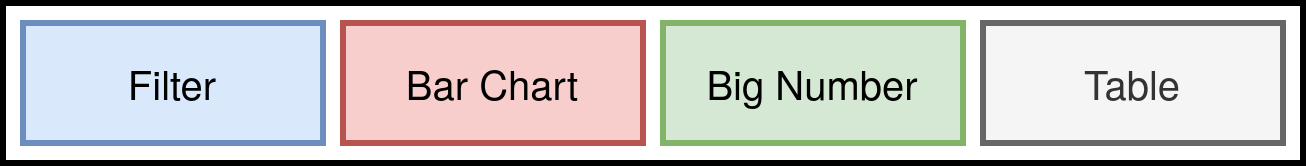
\includegraphics[width=1\linewidth]{images/dashboardsLayout} \caption{Example of a dashboards tool presenting the databases available in the network (simulated data)}\label{fig:dashboardsLayout}
\end{figure}

\hypertarget{license}{%
\subsection*{License}\label{license}}
\addcontentsline{toc}{subsection}{License}

The system is open-source
and this manual was written in \href{https://rmarkdown.rstudio.com}{RMarkdown} using the \href{https://bookdown.org}{bookdown} package.

\hypertarget{acknowledges}{%
\subsection*{Acknowledges}\label{acknowledges}}
\addcontentsline{toc}{subsection}{Acknowledges}

This work has been conducted in the context of EHDEN, a project that receives funding from the European Union's Horizon 2020 and EFPIA through IMI2 Joint Undertaking initiative, under grant agreement No 806968.

\hypertarget{introduction}{%
\chapter{Introduction}\label{introduction}}

The OHDSI research network has been growing steadily which results in an increasing number of healthcare databases standardized to the OMOP CDM format. The OHDSI community created the ACHILLES tool (Automated Characterization of Health Information at Large-scale Longitudinal Exploration System) to characterize those databases. The results are available to the data custodian in their local ATLAS tool and helps them to gain insights in their data and helps in assessing the feasibility of a particular research questions.

ACHILLES was designed to extract the metadata from a single database, which by itself does not allow the comparison with the remaining databases in the network. However, we believe there is even more value in sharing this information with others to enable network research in a Data Network Dashboard.

Data Network Dashboard

The European Health Data and Evidence Network (EHDEN) project therefore designed a Data Network Dashboard tool, a web application to aggregate information from distributed OMOP CDM databases. It uses the ACHILLES results files to construct graphical dashboards and enables database comparison (Figure \ref{fig:intro}). The tool is built on Apache Superset, which is an open-source enterprise-ready business intelligence web application that can provide powerful and fully customizable graphical representations of data. Achilles results can be uploaded through the EHDEN Database Catalogue using the dashboards plugin but can also be directly uploaded in the tool. Figure 1. Example of a dashboards tool presenting age and gender distributions (simulated data).

\begin{figure}
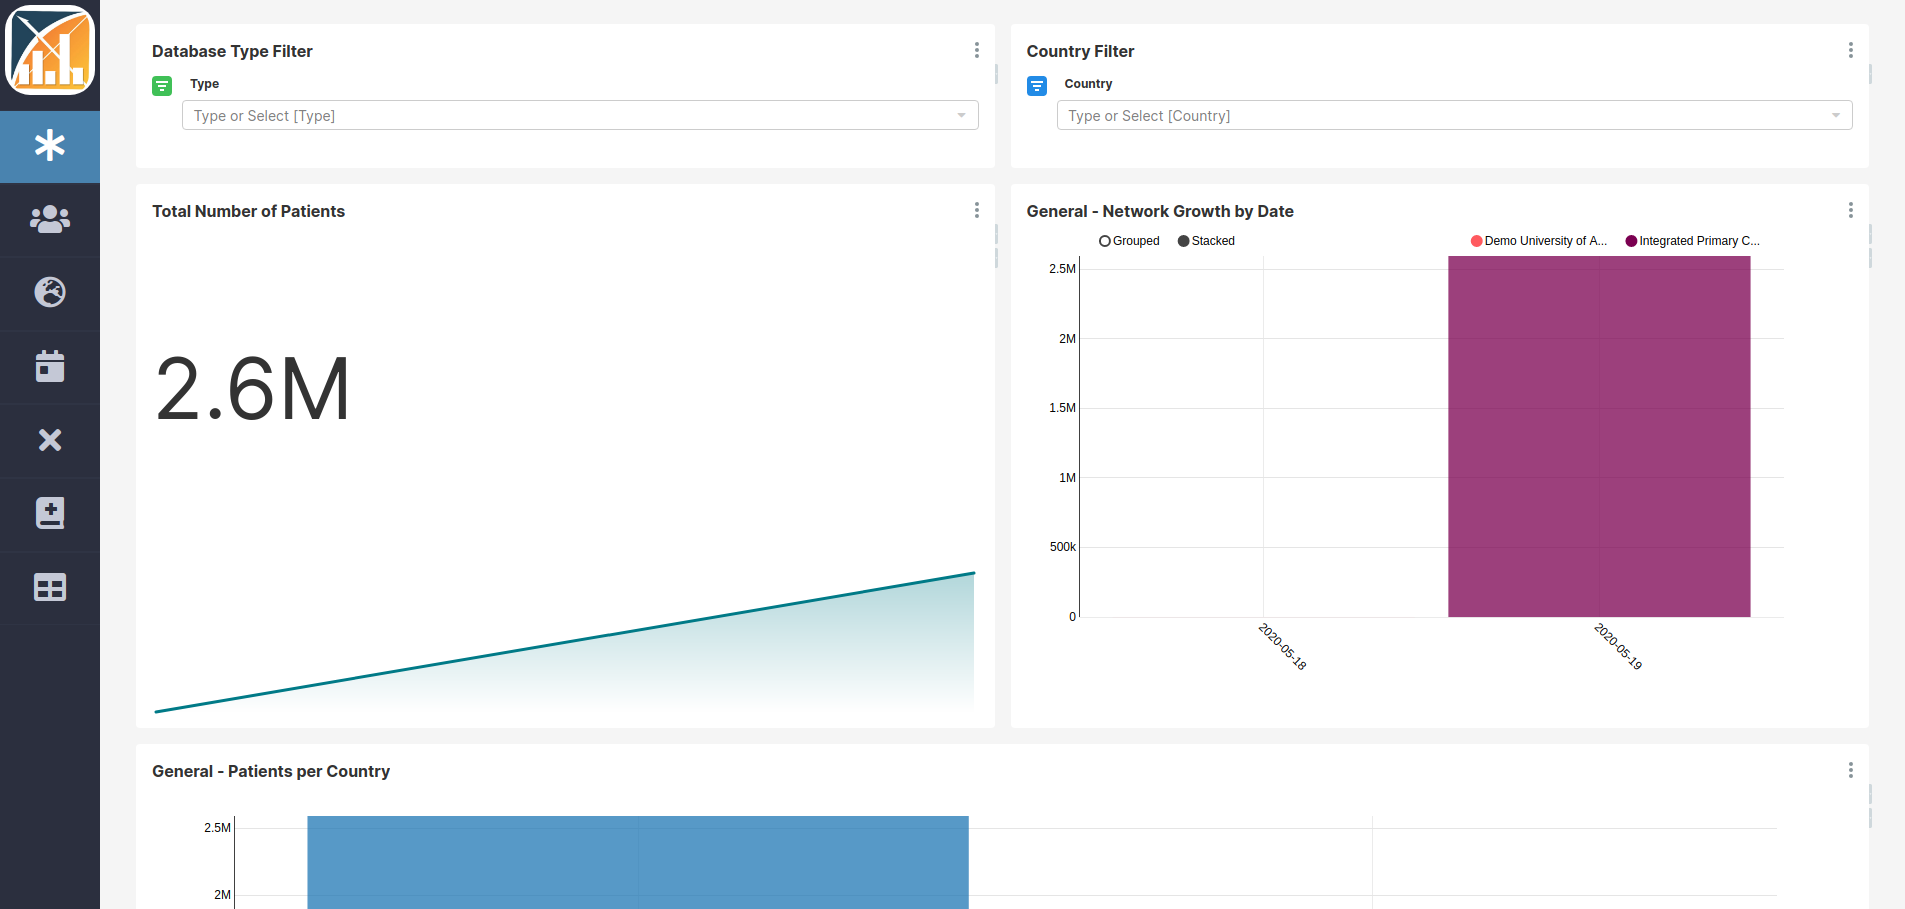
\includegraphics[width=1\linewidth]{images/01-intro} \caption{Example of a dashboards tool presenting the databases available in the network (simulated data)}\label{fig:intro}
\end{figure}

In this tools, we defined and implemented a series of charts and dashboards containing the most relevant information about the databases, such as:

\begin{itemize}
\tightlist
\item
  \textbf{General}: dashboards that shows the databases types per country, the distribution of data source types, the growth of the Network including the number of database and the number of patients in the databases over time;
\item
  \textbf{Person}: representing the number of patients per country, age distribution at first observation, year of birth distribution and normalized gender distribution;
\item
  \textbf{Population characteristics}: dashboard with the cumulative patient time, persons with continuous observation per month, and the start and end dates of those periods;
\item
  \textbf{Visit}: chart to compare the number and type of visit occurrence records;
\item
  \textbf{Death}: information about the number of death records by month, and the patient age at time of death;
\item
  \textbf{Concepts}: bubble chart which shows the number of patients and records per concept over the databases;
\item
  \textbf{Data domains}: heat map visualization of the major data domains in each database.
\end{itemize}

\hypertarget{installation}{%
\chapter{Installation}\label{installation}}

Currently, we use docker to deploy our environment

\hypertarget{first-steps}{%
\subsection*{First Steps}\label{first-steps}}
\addcontentsline{toc}{subsection}{First Steps}

\begin{enumerate}
\def\labelenumi{\arabic{enumi}.}
\item
  Clone the repository with the command \texttt{git\ clone\ -\/-recurse-submodules\ https://github.com/EHDEN/NetworkDashboards}. If you already cloned the repository without the \texttt{-\/-recurse-submodules} option, run \texttt{git\ submodule\ update\ -\/-init} to fetch the superset submodule.
\item
  Create a \texttt{.env} file on the \texttt{docker} directory, using \texttt{.env-example} as a reference, setting all necessary environment variables (\texttt{SUPERSET\textbackslash{}\_MAPBOX\textbackslash{}\_API\textbackslash{}\_KEY} and \texttt{DASHBOARD\textbackslash{}\_VIEWER\textbackslash{}\_SECRET\textbackslash{}\_KEY}).
\end{enumerate}

\hypertarget{dashboard-viewer-setup}{%
\subsection*{Dashboard Viewer setup}\label{dashboard-viewer-setup}}
\addcontentsline{toc}{subsection}{Dashboard Viewer setup}

\begin{enumerate}
\def\labelenumi{\arabic{enumi}.}
\item
  If you wish to expose the dashboard viewer app through a specific domain(s) you must add it/them to the \texttt{ALLOWED\_HOSTS} list on file \texttt{dashboard\_viewer/dashboard\_viewer/settings.py} and remove the \texttt{\textquotesingle{}*\textquotesingle{}} entry.
\item
  Build containers' images: \texttt{docker-compose\ build}. This might take several minutes.
\item
  Set up the database and create an admin account for the dashboard viewer app: \texttt{docker-compose\ run\ -\/-rm\ dashboard\ ./docker-init.sh}.
\end{enumerate}

\hypertarget{insert-concepts}{%
\subsection*{Insert Concepts}\label{insert-concepts}}
\addcontentsline{toc}{subsection}{Insert Concepts}

The concepts table is not in the repository due to its dimension, therefore we use directly the Postgres console to insert this table in the installation.

\begin{enumerate}
\def\labelenumi{\arabic{enumi}.}
\item
  Get your concept csv file from \href{https://athena.ohdsi.org/}{Athena}
\item
  Copy the file into postgres container

\begin{Shaded}
\begin{Highlighting}[]
\ExtensionTok{docker}\NormalTok{ cp concept.csv dashboard\_viewer\_postgres\_1:/tmp/}
\end{Highlighting}
\end{Shaded}
\item
  Enter in the postgres container:

\begin{Shaded}
\begin{Highlighting}[]
\ExtensionTok{docker}\NormalTok{ exec {-}it dashboard\_viewer\_postgres\_1 bash}
\end{Highlighting}
\end{Shaded}
\item
  Enter in the \texttt{achilles} database (value of the variable \texttt{POSTGRES\_ACHILLES\_DB} on the .env file) with the \texttt{root} user (value of the variable \texttt{POSTGRES\_ROOT\_USER} on the .env file):

\begin{verbatim}
psql achilles root
\end{verbatim}
\item
  Create the \texttt{concept} table

\begin{Shaded}
\begin{Highlighting}[]
\KeywordTok{CREATE} \KeywordTok{TABLE}\NormalTok{ concept (}
\NormalTok{  concept\_id         }\DataTypeTok{INTEGER}        \KeywordTok{NOT} \KeywordTok{NULL}\NormalTok{,}
\NormalTok{  concept\_name       }\DataTypeTok{VARCHAR}\NormalTok{(}\DecValTok{255}\NormalTok{)   }\KeywordTok{NOT} \KeywordTok{NULL}\NormalTok{,}
\NormalTok{  domain\_id          }\DataTypeTok{VARCHAR}\NormalTok{(}\DecValTok{20}\NormalTok{)    }\KeywordTok{NOT} \KeywordTok{NULL}\NormalTok{,}
\NormalTok{  vocabulary\_id      }\DataTypeTok{VARCHAR}\NormalTok{(}\DecValTok{20}\NormalTok{)    }\KeywordTok{NOT} \KeywordTok{NULL}\NormalTok{,}
\NormalTok{  concept\_class\_id   }\DataTypeTok{VARCHAR}\NormalTok{(}\DecValTok{20}\NormalTok{)    }\KeywordTok{NOT} \KeywordTok{NULL}\NormalTok{,}
\NormalTok{  standard\_concept   }\DataTypeTok{VARCHAR}\NormalTok{(}\DecValTok{1}\NormalTok{)     }\KeywordTok{NULL}\NormalTok{,}
\NormalTok{  concept\_code       }\DataTypeTok{VARCHAR}\NormalTok{(}\DecValTok{50}\NormalTok{)    }\KeywordTok{NOT} \KeywordTok{NULL}\NormalTok{,}
\NormalTok{  valid\_start\_date   }\DataTypeTok{DATE}           \KeywordTok{NOT} \KeywordTok{NULL}\NormalTok{,}
\NormalTok{  valid\_end\_date     }\DataTypeTok{DATE}           \KeywordTok{NOT} \KeywordTok{NULL}\NormalTok{,}
\NormalTok{  invalid\_reason     }\DataTypeTok{VARCHAR}\NormalTok{(}\DecValTok{1}\NormalTok{)     }\KeywordTok{NULL}
\NormalTok{);}
\end{Highlighting}
\end{Shaded}
\item
  Copy the CSV file content to the table (this could take a while)

  To get both \texttt{\textquotesingle{}} (single quotes) and \texttt{"} (double quotes) on the \texttt{concept\_name} column we use a workaround by setting the quote character to one that should never be in the text. Here we used \texttt{\textbackslash{}b} (backslash).

\begin{Shaded}
\begin{Highlighting}[]
\KeywordTok{COPY} \KeywordTok{public}\NormalTok{.concept }\KeywordTok{FROM} \StringTok{\textquotesingle{}/tmp/concept.csv\textquotesingle{}} \KeywordTok{WITH}\NormalTok{ CSV }\KeywordTok{HEADER}
\NormalTok{  DELIMITER E}\StringTok{\textquotesingle{}}\CharTok{\textbackslash{}t}\StringTok{\textquotesingle{}}\NormalTok{ QUOTE E}\StringTok{\textquotesingle{}}\CharTok{\textbackslash{}b}\StringTok{\textquotesingle{}}\NormalTok{;}
\end{Highlighting}
\end{Shaded}
\item
  Create index in table (this could take a while):

\begin{Shaded}
\begin{Highlighting}[]
\KeywordTok{CREATE} \KeywordTok{INDEX}\NormalTok{ concept\_concept\_id\_index }\KeywordTok{ON}\NormalTok{ concept (concept\_id);}
\KeywordTok{CREATE} \KeywordTok{INDEX}\NormalTok{ concept\_concept\_name\_index }\KeywordTok{ON}\NormalTok{ concept (concept\_name);}
\end{Highlighting}
\end{Shaded}
\item
  Set the owner of the \texttt{concept} table to the \texttt{achilles} user (value of the variable \texttt{POSTGRES\_ACHILLES\_USER} on the .env file):

\begin{verbatim}
ALTER TABLE concept OWNER TO achiller
\end{verbatim}
\item
  Bring up the containers: \texttt{docker-compose\ up\ -d}.
\item
  Run the command \texttt{docker-compose\ run\ -\/-rm\ dashboard\ python\ manage.py\ generate\_materialized\_views} to create the materialized views on Postgres.
\end{enumerate}

\hypertarget{superset-setup}{%
\subsection*{Superset setup}\label{superset-setup}}
\addcontentsline{toc}{subsection}{Superset setup}

\begin{enumerate}
\def\labelenumi{\arabic{enumi}.}
\item
  Make sure that the container \texttt{superset-init} has finished before continuing. It is creating the necessary tables on the database and creating permissions and roles.
\item
  Execute the script \texttt{./superset/one\_time\_run\_scripts/superset-init.sh}. This will create an admin account and associate the~\texttt{achilles}~database to Superset.~\textbf{Attention:}~You must be in the docker directory to execute this script.
\item
  We have already built some dashboards so if you want to import them run the script \texttt{./superset/one\_time\_run\_scripts/load\_dashboards.sh}. \textbf{Attention:} You must be in the docker directory to execute this script.
\item
  If you used the default ports:

  \begin{itemize}
  \tightlist
  \item
    Go to \texttt{http://localhost} to access the dashboard viewer app.
  \item
    Go to \texttt{http://localhost:8088} to access superset.
  \end{itemize}
\item
  To any anonymous user view dashboards, add the following:

  \begin{itemize}
  \tightlist
  \item
    all datasource access on all\_datasource\_access
  \item
    can csrf token on Superset
  \item
    can dashboard on Superset
  \item
    can explore json on Superset
  \item
    can read on Chart
  \item
    can read on CssTemplate
  \end{itemize}
\end{enumerate}

\hypertarget{dummy-data}{%
\subsection*{Dummy data}\label{dummy-data}}
\addcontentsline{toc}{subsection}{Dummy data}

On a fresh installation, there are no achilles\_results data so Superset's dashboards will display ``No results''. On the root of this repository, you can find the \texttt{demo} directory where we have an ACHILLES results file with synthetic data that you can upload to a data source on the uploader app of the dashboard viewer (\url{http://localhost/uploader}). If you wish to compare multiple data sources, on the \texttt{demo} directory there is also a python script that allows you to generate new ACHILLES results files, where it generates random count values based on the ranges of values for each set of analysis\_id and stratums present on a base ACHILLES results file. So, from the one ACHILLES results fill we provided, you can have multiple data sources with different data.

\hypertarget{processes}{%
\chapter{Processes}\label{processes}}

\hypertarget{data-sources}{%
\subsection*{Data Sources}\label{data-sources}}
\addcontentsline{toc}{subsection}{Data Sources}

\textbf{Target: platform user}

Before uploading any data to this platform, a data source owner has to create a data source instance to then associated the upload data with.

The creation of data source is done through the \texttt{{[}BASE\_URL{]}/uploader/} URL, where 7 fields are expected:

\begin{enumerate}
\def\labelenumi{\arabic{enumi}.}
\tightlist
\item
  name: an extensive name
\item
  acronym: a short name
\item
  country: where is the data source localized
\item
  link (Optional): web page of the data source
\item
  database type: type of OMOP database
\item
  coordinates: a more accurate representation of the data source's localization
\item
  hash (Optional): the internal unique identifier of a data source
\end{enumerate}

If you access \texttt{{[}BASE\_URL{]}/uploader/} the 7th field (hash) is set automatically for something random, however, if you want to set it use the \texttt{{[}BASE\_URL{]}/uploader/{[}HASH{]}/} URL.

To avoid duplication on the database type field, this field is transformed (use title case and trimmed) and then is checked there is already a record (Database Type) with the same value.

There are several ways to create a data source:

\begin{enumerate}
\def\labelenumi{\arabic{enumi}.}
\tightlist
\item
  Create through a web form
\end{enumerate}

By accessing the \texttt{{[}BASE\_URL{]}/uploader/} URL, you will get a form where you can field the fields, where the country field is a dropdown and the coordinates field is set through a map widget.

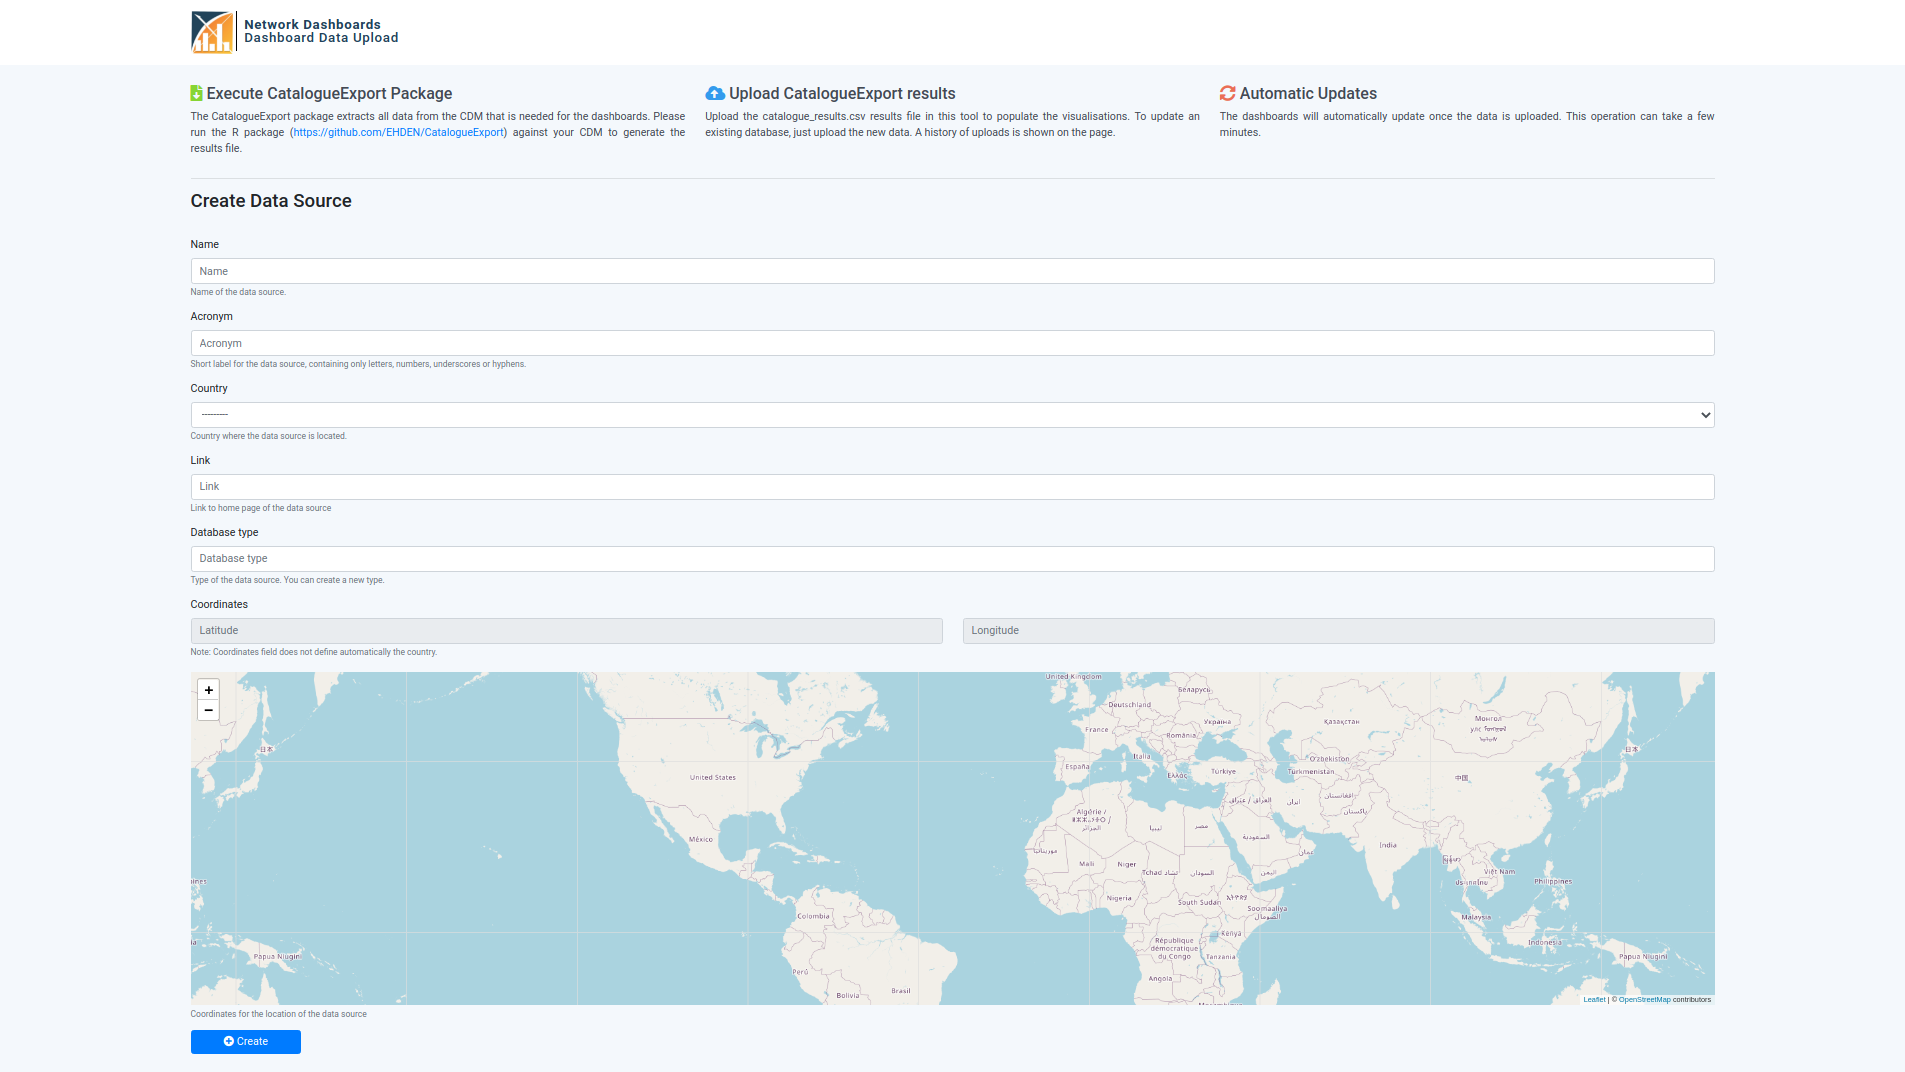
\includegraphics{images/processes/processes_data_source_creation.png}

\begin{enumerate}
\def\labelenumi{\arabic{enumi}.}
\setcounter{enumi}{1}
\tightlist
\item
  Automatically create when performing a GET to the \texttt{{[}BASE\_URL{]}/uploader/} URL
\end{enumerate}

If the Network Dashboards platform is being used as a third-party application and the main application has all the data for the required fields, the data source can be automatically created and the user is redirected directly to the upload files page.

To perform this, each field should be provided as a URL parameter when accessing the \texttt{{[}BASE\_URL{]}/uploader/} URL. If all required fields are provided and are valid the data source is created and the user is redirected to the upload files page. If a required field is missing or is not valid the webform is presented to the user so it can manually fill those fields.

\begin{enumerate}
\def\labelenumi{\arabic{enumi}.}
\setcounter{enumi}{2}
\tightlist
\item
  Automatically create by performing a POST to the \texttt{{[}BASE\_URL{]}/uploader/} URL
\end{enumerate}

Since the creation URL does not have csrf cookie protection, you can perform a POST request as you were submitting a form.

\textbf{Notes For the automatic options}:
-. Since the coordinates field is composed of two fields (latitude, longitude), it should be submitted as \texttt{coordinates\_0={[}latitude{]}} and \texttt{coordinates\_1={[}longitude{]}}
-. The country field should match one of the available on the dropdown of the webform.

\hypertarget{catalogue-results-files}{%
\subsection*{Catalogue Results Files}\label{catalogue-results-files}}
\addcontentsline{toc}{subsection}{Catalogue Results Files}

\textbf{Target: platform user}

Once a data source is created you can access its upload page by accessing the \texttt{{[}BASE\_URL{]}/uploader/{[}HASH{]}/}. If no data source has the provided hash you will be redirected back to the data source creation form.

On the upload page you can:

\begin{enumerate}
\def\labelenumi{\arabic{enumi}.}
\tightlist
\item
  Go to the edit page of your data source
\item
  Upload a catalogue results file
\item
  Check the upload history
\end{enumerate}

A catalogue results file is a CSV file, the result obtained after running the \href{https://github.com/EHDEN/CatalogueExport}{EHDEN/CatalogueExport} R package on an OMOP database. It is a variant of the \href{https://github.com/OHDSI/Achilles}{OHDSI/Achilles} where it only extracts a subset of analyses of the ACHILLES' original set.

The upload form expects a CSV file with the following columns:

\begin{longtable}[]{@{}lll@{}}
\toprule
Name & Type & Required/Non-Nullable/Non-Empty\tabularnewline
\midrule
\endhead
analysis\_id & int & Yes\tabularnewline
stratum\_1 & string & No\tabularnewline
stratum\_2 & string & No\tabularnewline
stratum\_3 & string & No\tabularnewline
stratum\_4 & string & No\tabularnewline
stratum\_5 & string & No\tabularnewline
count\_value & int & Yes\tabularnewline
min\_value & double & No\tabularnewline
max\_value & double & No\tabularnewline
avg\_value & double & No\tabularnewline
stdev\_value & double & No\tabularnewline
median\_value & double & No\tabularnewline
p10\_value & double & No\tabularnewline
p25\_value & double & No\tabularnewline
p75\_value & double & No\tabularnewline
p90\_value & double & No\tabularnewline
\bottomrule
\end{longtable}

The uploaded file must:

\begin{itemize}
\item
  either contain the first 7 columns OR all 16 columns
\item
  contain the columns in the same order as presented in the table above
\end{itemize}

While parsing the uploaded file, some data is extracted to then present on the Upload history and to update data source information. This data is extracted from the record with analysis id 0, \textbf{which is required to be present on the file}, and 5000, which is optional. Next is presented the data extracted and their description:

\begin{itemize}
\item
  R Package Version: the version of CatalogueExport R package used
\item
  Generation Date: date at which the CatalogueExport was executed on the OMOP database
\item
  Source Release Date: date at which the OMOP database was released
\item
  CDM Release Date: date at which the used CDM version was released
\item
  CDM Version: version of the CDM used
\item
  Vocabulary Version: version of the vocabulary used
\end{itemize}

The next table is presented where the previous data is stored on the rows with analysis id 0 and 5000:

\begin{longtable}[]{@{}llllll@{}}
\toprule
Analysis Id & Stratum 1 & Stratum 2 & Stratum 3 & Stratum 4 & Stratum 5\tabularnewline
\midrule
\endhead
0 & & R Package Version & Generation Date & &\tabularnewline
5000 & & Source Release Date & CDM Release Date & CDM Version & Vocabulary Version\tabularnewline
\bottomrule
\end{longtable}

\hypertarget{materialized-views}{%
\subsection*{Materialized Views}\label{materialized-views}}
\addcontentsline{toc}{subsection}{Materialized Views}

\textbf{Target: admin user}

For each chart, Superset has an underlying SQL query which in our case is run every time a chart is rendered. If one of these queries takes too long to execute the charts will also take too long until they are rendered and eventually users might get timeout messages given a bad user experience.

To avoid this problem, instead of executing the raw SQL query we create a \href{https://www.postgresql.org/docs/10/rules-materializedviews.html}{postgres materialized view} of the query, which is then used to feed the data to the chart. So only a simple \texttt{SELECT\ x\ FROM\ x} query is executed when a chart is rendered.

So whenever I create a chart I have to access the Postgres console? No, we created an unmanaged Materialized Queries model that maps to the materialized views on Postgres. With it you can create new materialized views through the Django admin app, by accessing the \texttt{{[}BASE\_URL{]}/admin/} URL.

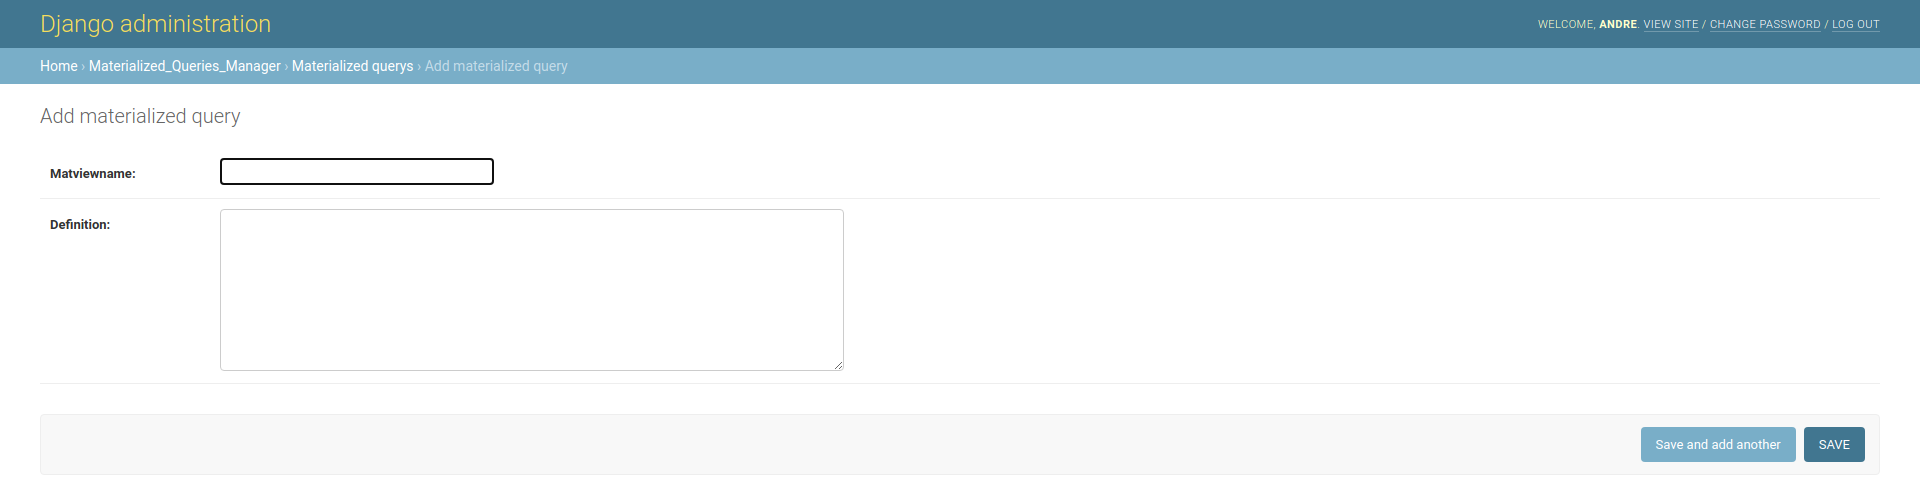
\includegraphics{images/processes/processes_materialized_view_creation.png}

You have to provide the materialized view name and its query, which will then be used to execute the query \texttt{CREATE\ MATERIALIZED\ VIEW\ {[}name{]}\ AS\ {[}query{]}}, which will be executed on a background task so the browser doesn't hang and times out, in case of complicated queries. Taking this into account, the record associated will not appear on the Django admin app until the \texttt{CREATE\ MATERIALIZED\ VIEW} query finishes.

To give feedback on the background task we use \href{https://github.com/celery/django-celery-results}{celery/django-celery-results}, so you can check the status of a task on the Task Results model of the Celery Results app

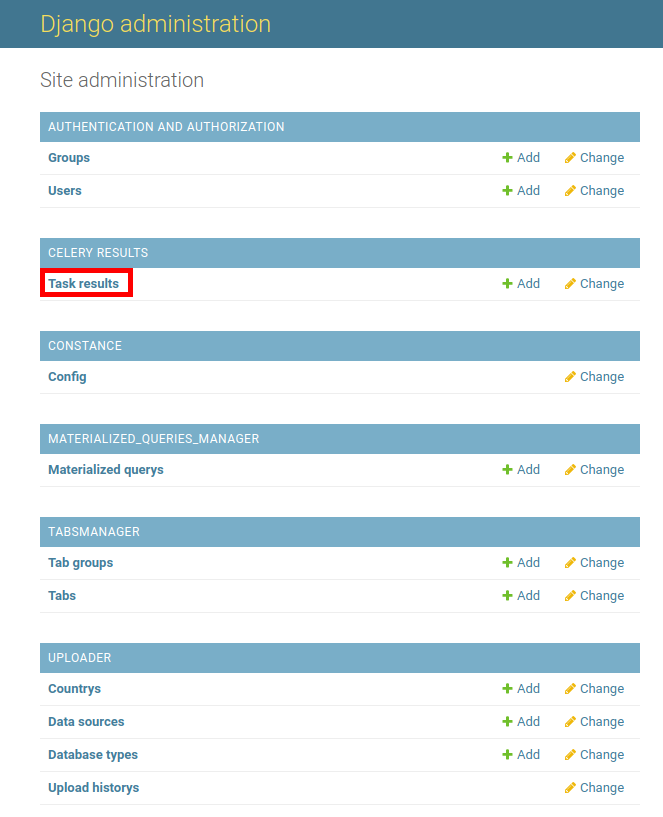
\includegraphics{images/processes/processes_task_results.png}

After the creation of a Materialized Query, the will be a message telling the id of the task which is executing the \texttt{CREATE\ MATERIALIZED\ VIEW} query. You can then check for the record associated with the task, click on the id to get more details. If something went wrong check the error message either on Result Data or Traceback fields under the Result section

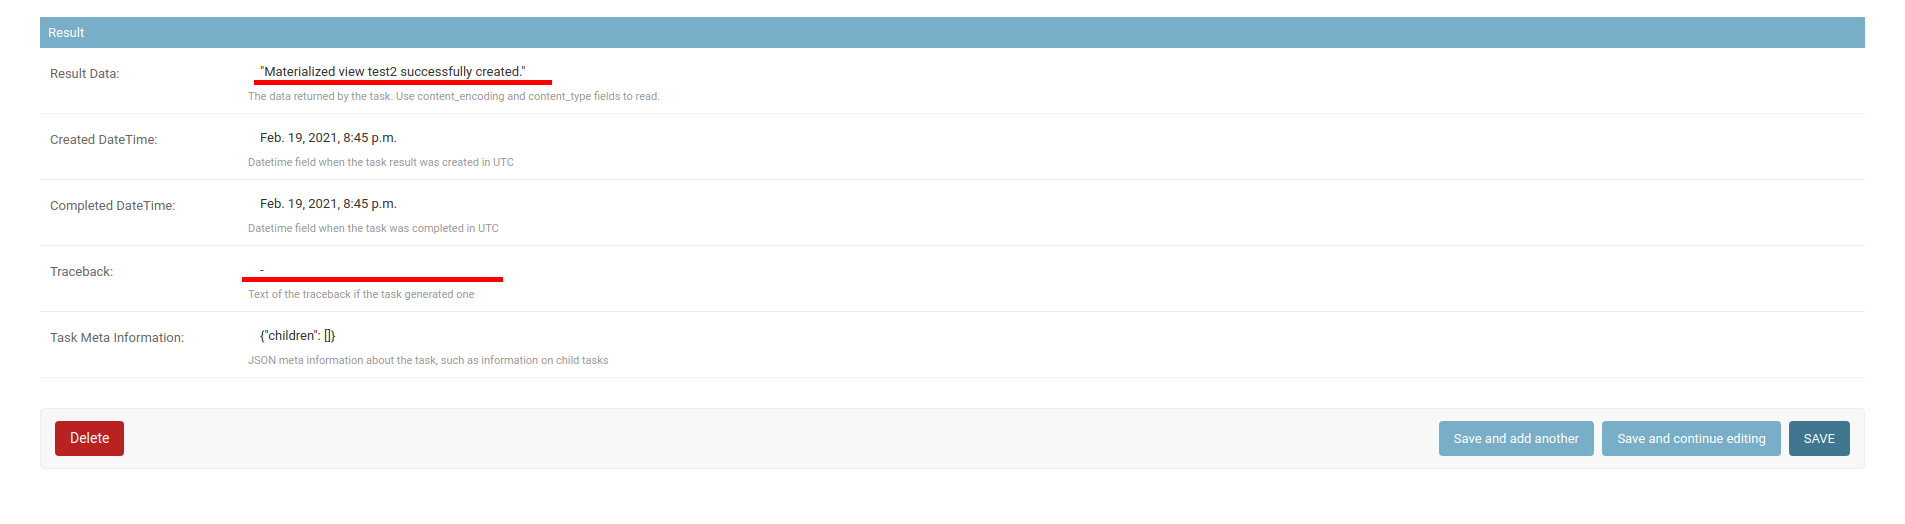
\includegraphics{images/processes/processes_task_result_info.png}

After all this, the final step is to add the materialized view as a Dataset. Login into Superset, then go to Data -\textgreater{} Datasets and create a new one. Select the \texttt{Achilles} database, the \texttt{public} schema, then the created materialized view and click ``ADD''. After this, the materialized view can be used as a data source for a new chart.

\hypertarget{tabs-view-deprecated}{%
\subsection*{Tabs View {[}Deprecated{]}}\label{tabs-view-deprecated}}
\addcontentsline{toc}{subsection}{Tabs View {[}Deprecated{]}}

\textbf{Target: admin user}

\hypertarget{backups}{%
\chapter{Backups}\label{backups}}

\begin{enumerate}
\def\labelenumi{\arabic{enumi}.}
\item
  Create a credentials file (the structure of the file depends on the target cloud server)
\item
  Create a \texttt{.dashboards\_backups.conf} file under your home directory (variable \texttt{\$HOME}) using \texttt{dashboards\_backups.conf.example} as base, setting the appropriate value for the several variables.

  For variables associated with files and directories always use \emph{absolute} paths.

  Variables:

  \begin{itemize}
  \item
    \texttt{RUN}: Set it to \texttt{0} if you don't want the next scheduled backup to run.

    This variable allows you to cancel any backup runs while you are doing some maintenance on the application.
  \item
    \texttt{CONSTANCE\_REDIS\_DB}: Number of the Redis database where the django constance config is stored. The default value is 2. This value should be the same as the environment variable \texttt{REDIS\_CONSTANCE\_DB} of the dashboard container.
  \item
    The following variables are associated with the arguemtns of the \texttt{backup\_uploader} python package. Check its \href{https://github.com/aspedrosa/BackupUploader\#usage}{usage} for more details:

    \begin{itemize}
    \item
      \texttt{APP\_NAME}: The backup process will generate some directories with this name in places that are shared with other applications.
    \item
      \texttt{SERVER}: The name of the target cloud server to where backups should be uploaded (dropbox or mega).
    \item
      \texttt{BACKUP\_CHAIN\_CONFIG}: Allows having different directories with backups of different ages.
    \item
      \texttt{CREDENTIALS\_FILE\_PATH}: File containing the credentials to access the server to upload the backup file.
    \end{itemize}
  \end{itemize}
\item
  Install the \texttt{backup\_uploader} python package by following its \href{https://github.com/aspedrosa/BackupUploader\#install}{install} instructions.
\item
  Schedule your backups

\begin{Shaded}
\begin{Highlighting}[]
\ExtensionTok{*}\NormalTok{    *    *   *    *  Command\_to\_execute}
\KeywordTok{|}    \KeywordTok{|}    \KeywordTok{|}    \KeywordTok{|}   \KeywordTok{|}       
\KeywordTok{|}    \KeywordTok{|}    \KeywordTok{|}    \KeywordTok{|}    \ExtensionTok{Day}\NormalTok{ of the Week ( 0 {-} 6 ) }\KeywordTok{(} \ExtensionTok{Sunday}\NormalTok{ = 0 }\KeywordTok{)}
\KeywordTok{|}    \KeywordTok{|}    \KeywordTok{|}    \KeywordTok{|}
\KeywordTok{|}    \KeywordTok{|}    \KeywordTok{|}    \ExtensionTok{Month}\NormalTok{ ( 1 {-} 12 )}
\KeywordTok{|}    \KeywordTok{|}    \KeywordTok{|}
\KeywordTok{|}    \KeywordTok{|}    \ExtensionTok{Day}\NormalTok{ of Month ( 1 {-} 31 )}
\KeywordTok{|}    \KeywordTok{|}
\KeywordTok{|}    \ExtensionTok{Hour}\NormalTok{ ( 0 {-} 23 )}
\KeywordTok{|}
\ExtensionTok{Min}\NormalTok{ ( 0 {-} 59 ) }
\end{Highlighting}
\end{Shaded}

  (Retrived from: \href{https://www.tutorialspoint.com/unix_commands/crontab.htm}{Tutorialspoint})

  Ex: To run every day at 3:00 am

  \begin{enumerate}
  \def\labelenumii{\arabic{enumii}.}
  \item
    \texttt{crontab\ -e}
  \item
    Add entry \texttt{0\ 3\ *\ *\ *\ \$HOME/NetworkDashboards/backups/backup.sh} (The path to the backup script might be different)
  \end{enumerate}
\end{enumerate}

\hypertarget{restore}{%
\section{Restore}\label{restore}}

\begin{enumerate}
\def\labelenumi{\arabic{enumi}.}
\item
  Select the compressed backup you want to restore and decompress it:

  \texttt{tar\ -xJf\ BACKUP\_FILE.tar.xz}.
\item
  \begin{enumerate}
  \def\labelenumii{\arabic{enumii}.}
  \item
    \textbf{Redis}

    \begin{enumerate}
    \def\labelenumiii{\arabic{enumiii}.}
    \item
      Make sure the redis docker container is down.
    \item
      (Re)place the file \texttt{dump.rdb} on the redis volume by the file \texttt{redis.rdb}. By default the redis volume is located where this repository was cloned on the directory \texttt{docker/volumes/redis}.
    \item
      Change its permissions, owner and group:

\begin{verbatim}
chmod 0644 docker/volumes/redis/dump.rdb
sudo chown -R 999:999 docker/volumes/redis
\end{verbatim}
    \end{enumerate}
  \item
    \textbf{Postgres}

    \begin{enumerate}
    \def\labelenumiii{\arabic{enumiii}.}
    \item
      Make sure all containers that make changes on the database are stopped.
    \item
      Copy the file \texttt{postgres\_backup.sql} into the postgres container

      \texttt{docker\ cp\ postgres.sql\ {[}CONTAINER\_ID{]}:/tmp}.
    \item
      Execute the backup script:

      \texttt{docker\ exec\ -u\ root\ dashboard\_viewer\_postgres\_1\ psql\ -f\ /tmp/postgres\_backup.sql\ -U\ \textbackslash{}\$POSTGRES\_USER\ -d\ \textbackslash{}\$POSTGRES\_DB}.
    \end{enumerate}
  \item
    \textbf{Media Files} If you have a volume pointing to where the media files are stored, replace all files with the ones present on the downloaded backup file. Else:

    \begin{enumerate}
    \def\labelenumiii{\arabic{enumiii}.}
    \item
      Bring the dashoard container up \texttt{docker-compose\ up\ -d\ dashboard}
    \item
      Enter in the container \texttt{docker\ exec\ -it\ {[}CONTAINER\_ID{]}\ bash}
    \item
      If you don't know where the media files are stored you can check the value of the MEDIA\_ROOT variable

      \begin{enumerate}
      \def\labelenumiv{\arabic{enumiv}.}
      \item
        \texttt{python\ manage.py\ shell}
      \item
        \texttt{from\ django.conf\ import\ settings}
      \item
        \texttt{print(settings.MEDIA\_ROOT)}
      \end{enumerate}
    \item
      Remove the entire MEDIA\_ROOT directory and exit the container
    \item
      Copy the media directory present on the backup file to the catalogue container \texttt{docker\ cp\ -a\ collected-media\ {[}CONTAINER\_ID{]}:{[}MEDIA\_ROOT\_PARENT\_PATH{]}}
    \end{enumerate}
  \end{enumerate}
\end{enumerate}

\hypertarget{customizations}{%
\chapter{Customizations}\label{customizations}}

\hypertarget{logo}{%
\subsection*{Logo}\label{logo}}
\addcontentsline{toc}{subsection}{Logo}

\hypertarget{uploader-page-texts}{%
\subsection*{Uploader Page Texts}\label{uploader-page-texts}}
\addcontentsline{toc}{subsection}{Uploader Page Texts}

\hypertarget{dashboards}{%
\chapter{Dashboards}\label{dashboards}}

\hypertarget{PerDatabaseDashboard}{%
\section{Per Database}\label{PerDatabaseDashboard}}

\hypertarget{label-colors}{%
\subsection*{Label Colors}\label{label-colors}}
\addcontentsline{toc}{subsection}{Label Colors}

In order to obtain the colors blue and rose in the chart representing the gender distribution,
add the following JSON entry to the JSON object of the \texttt{JSON\ Metadata} field on the edit dashboard page:

\begin{Shaded}
\begin{Highlighting}[]
\ErrorTok{"label\_colors":} \FunctionTok{\{}
    \DataTypeTok{"Male"}\FunctionTok{:} \StringTok{"\#3366FF"}\FunctionTok{,} 
    \DataTypeTok{"Female"}\FunctionTok{:} \StringTok{"\#FF3399"}
\FunctionTok{\}}
\end{Highlighting}
\end{Shaded}

\hypertarget{css}{%
\subsection*{CSS}\label{css}}
\addcontentsline{toc}{subsection}{CSS}

To hide the dashboard header insert the following css code to the \texttt{CSS} field on the edit page:

\begin{Shaded}
\begin{Highlighting}[]
\FunctionTok{.dashboard} \OperatorTok{\textgreater{}}\NormalTok{ div}\InformationTok{:not(}\FunctionTok{.dashboard{-}content}\InformationTok{)}\NormalTok{ \{  }\CommentTok{/* dashboard header */}
  \KeywordTok{display}\NormalTok{: }\DecValTok{none}\OperatorTok{;}
\NormalTok{\}}
\end{Highlighting}
\end{Shaded}

With this every time you want to edit the dashboard layout you have to either comment the CSS inserted
or remove it so the ``Edit Dashboard'' button can show again.

\hypertarget{data-source-filter}{%
\subsection*{Data Source Filter}\label{data-source-filter}}
\addcontentsline{toc}{subsection}{Data Source Filter}

\begin{figure}
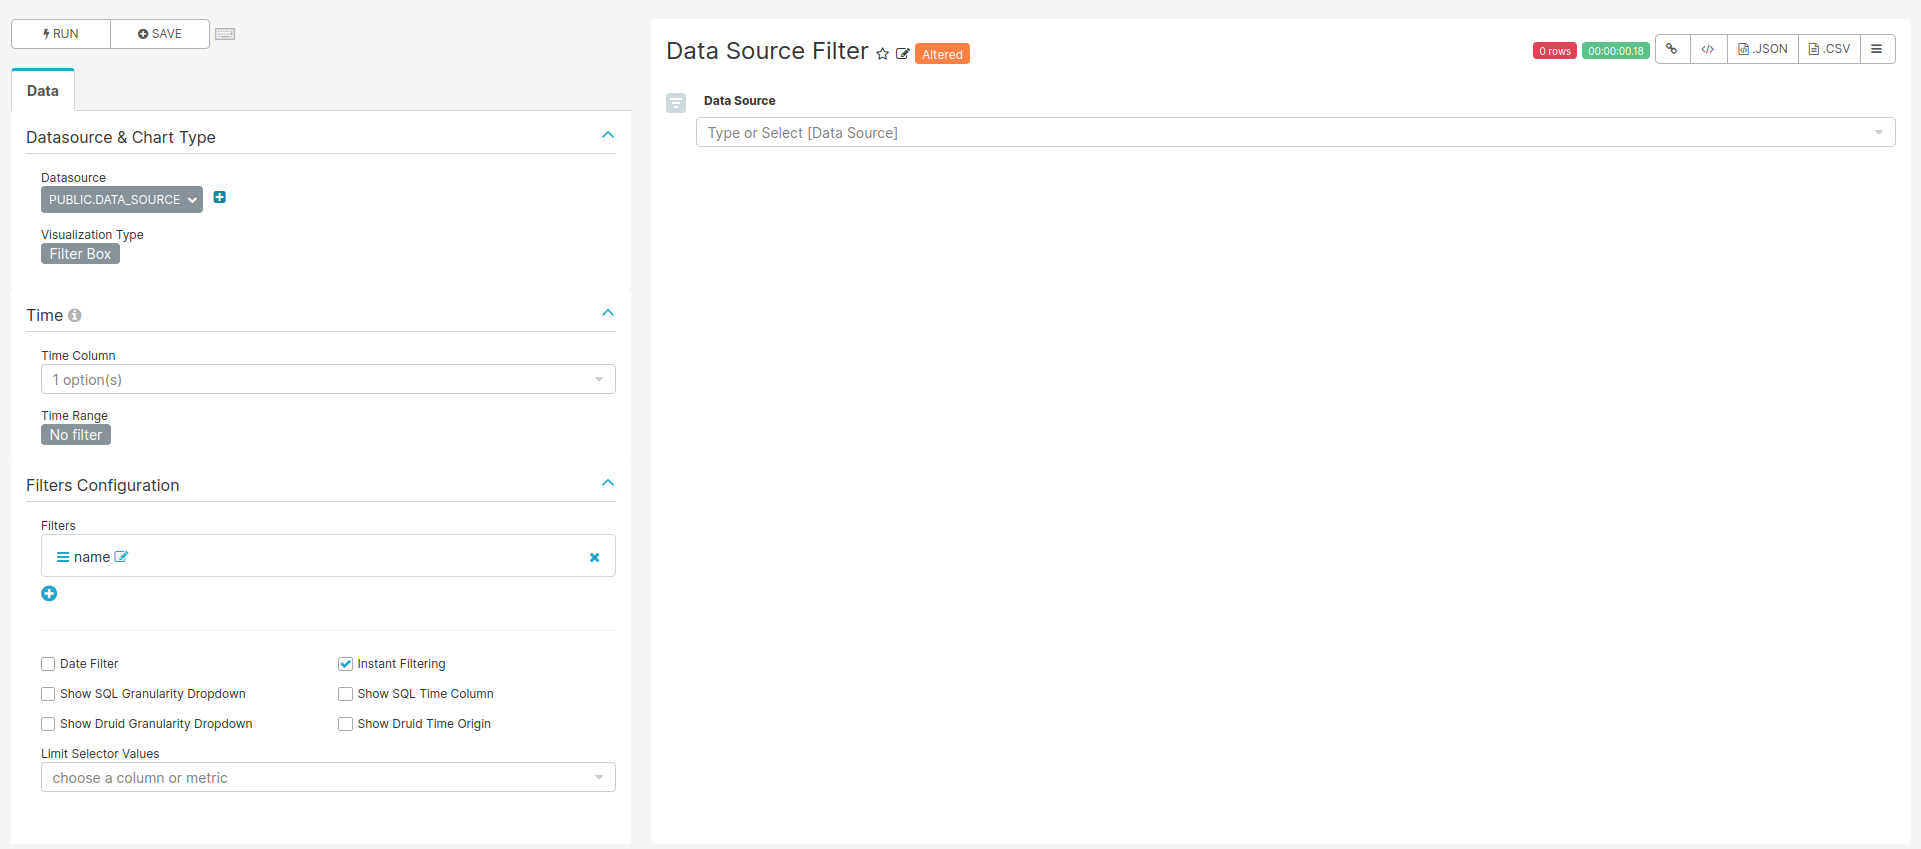
\includegraphics[width=1\linewidth]{images/shared/data_source_filter} \caption{Settings for creating the Data Source filter chart}\label{fig:dataSourceFilter}
\end{figure}

\textbf{For the filter to work the name of the fields to filter should match in all tables used on the charts of this dashboard.}

\hypertarget{sql-query}{%
\subsubsection*{SQL query}\label{sql-query}}
\addcontentsline{toc}{subsubsection}{SQL query}

No SQL query, use the sql table \texttt{data\_source} of the \texttt{achilles} database.

\hypertarget{chart-settings}{%
\subsubsection*{Chart settings}\label{chart-settings}}
\addcontentsline{toc}{subsubsection}{Chart settings}

\begin{itemize}
\tightlist
\item
  Data Tab

  \begin{itemize}
  \tightlist
  \item
    Datasource \& Chart Type

    \begin{itemize}
    \tightlist
    \item
      Visualization Type: Filter Box
    \end{itemize}
  \item
    Time

    \begin{itemize}
    \tightlist
    \item
      Time range: No filter
    \end{itemize}
  \item
    Filters Configuration

    \begin{itemize}
    \tightlist
    \item
      Filters:

      \begin{itemize}
      \tightlist
      \item
        name
      \end{itemize}
    \item
      Date Filter: off
    \item
      Instant Filtering: on
    \end{itemize}
  \end{itemize}
\end{itemize}

\hypertarget{demographics-tab}{%
\subsection*{Demographics Tab}\label{demographics-tab}}
\addcontentsline{toc}{subsection}{Demographics Tab}

\hypertarget{number-of-patients}{%
\subsubsection*{Number of Patients}\label{number-of-patients}}
\addcontentsline{toc}{subsubsection}{Number of Patients}

\begin{figure}
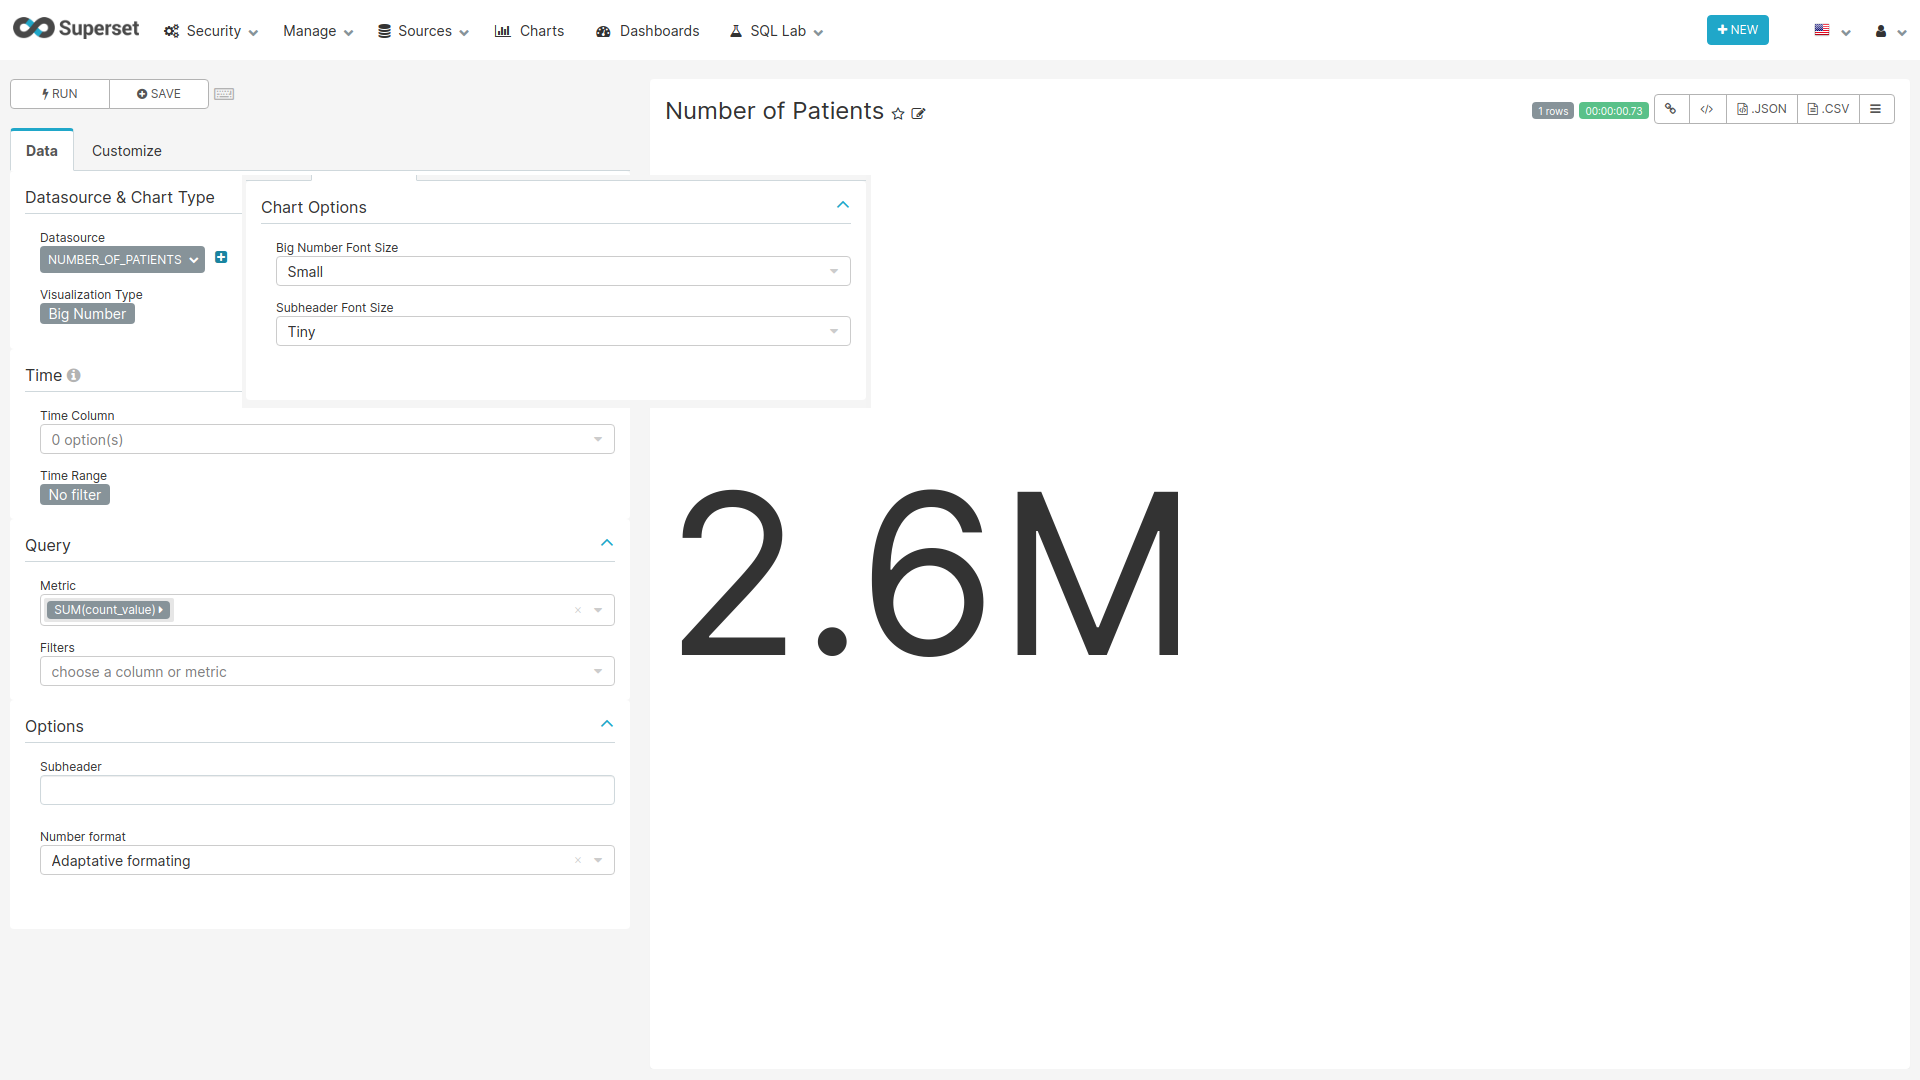
\includegraphics[width=1\linewidth]{images/11-per_database/01-demographics/01-num_patients} \caption{Settings for creating the Number of Patients chart}\label{fig:numPatients}
\end{figure}

\hypertarget{sql-query-1}{%
\paragraph*{SQL query}\label{sql-query-1}}
\addcontentsline{toc}{paragraph}{SQL query}

\begin{Shaded}
\begin{Highlighting}[]
\KeywordTok{SELECT}
\NormalTok{  achilles\_results.count\_value,}
\NormalTok{  data\_source.name,}
\NormalTok{  data\_source.acronym}
\KeywordTok{FROM}\NormalTok{ achilles\_results}
\KeywordTok{JOIN}\NormalTok{ data\_source }\KeywordTok{ON}\NormalTok{ achilles\_results.data\_source\_id}\OperatorTok{=}\NormalTok{data\_source.}\KeywordTok{id}
\KeywordTok{WHERE}\NormalTok{ analysis\_id }\OperatorTok{=} \DecValTok{1}
\end{Highlighting}
\end{Shaded}

\hypertarget{chart-settings-1}{%
\paragraph*{Chart settings}\label{chart-settings-1}}
\addcontentsline{toc}{paragraph}{Chart settings}

\begin{itemize}
\tightlist
\item
  Data Tab

  \begin{itemize}
  \tightlist
  \item
    Datasource \& Chart Type

    \begin{itemize}
    \tightlist
    \item
      Visualization Type: Big Number
    \end{itemize}
  \item
    Time
    Time range: No filter
  \item
    Query

    \begin{itemize}
    \tightlist
    \item
      Metric: sum(count\_value)
    \end{itemize}
  \end{itemize}
\item
  Customize Tab

  \begin{itemize}
  \tightlist
  \item
    Big Number Font Size: Small
  \item
    Subheader Font Size: Tiny
  \end{itemize}
\end{itemize}

\hypertarget{gender-table}{%
\subsubsection*{Gender Table}\label{gender-table}}
\addcontentsline{toc}{subsubsection}{Gender Table}

\begin{figure}
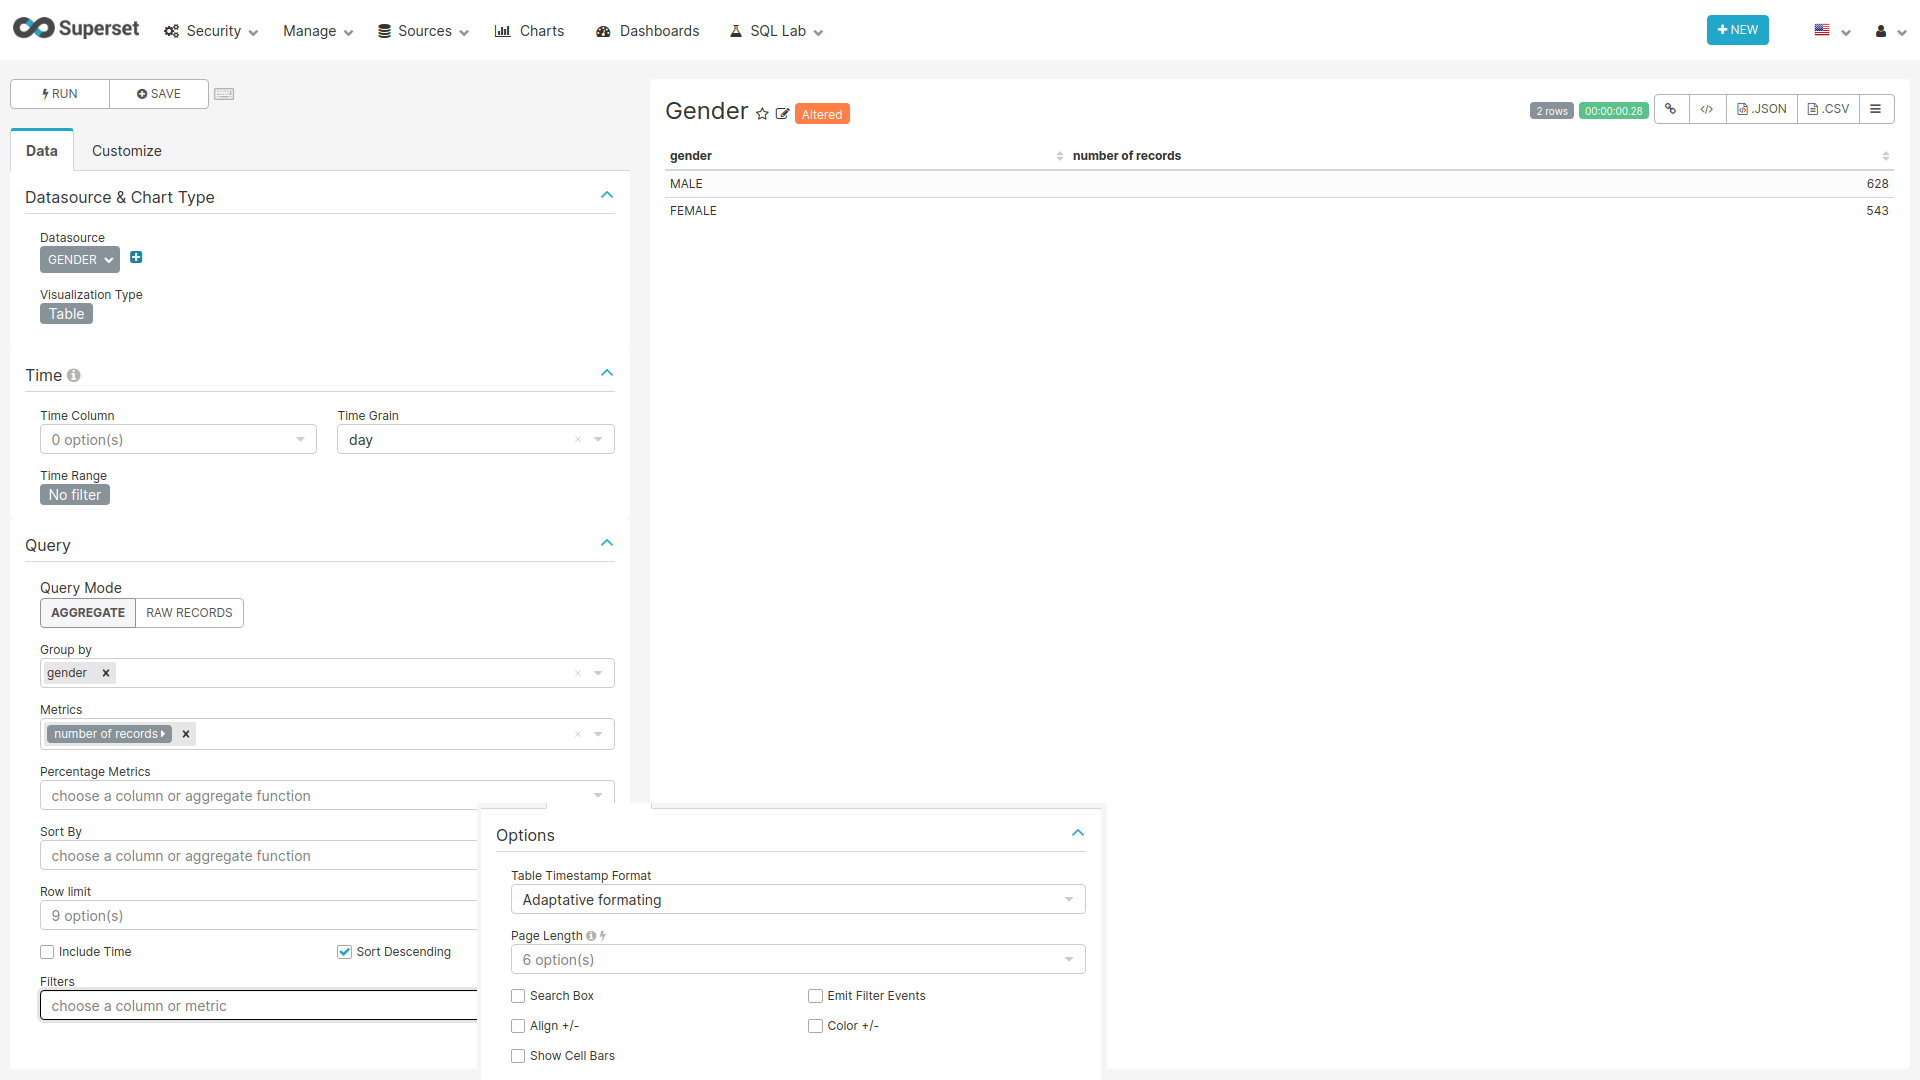
\includegraphics[width=1\linewidth]{images/11-per_database/01-demographics/02-gender_table} \caption{Settings for creating the Gender Table chart}\label{fig:genderTable}
\end{figure}

\hypertarget{sql-query-gendertablequery}{%
\paragraph*{SQL Query \{\#genderTableQuery\}}\label{sql-query-gendertablequery}}
\addcontentsline{toc}{paragraph}{SQL Query \{\#genderTableQuery\}}

\begin{Shaded}
\begin{Highlighting}[]
\KeywordTok{SELECT} \KeywordTok{source}\NormalTok{.name }\KeywordTok{as}\NormalTok{ name,}
       \KeywordTok{source}\NormalTok{.acronym,}
\NormalTok{       concept\_name }\KeywordTok{as}\NormalTok{ gender,}
\NormalTok{       count\_value}
\KeywordTok{FROM} \KeywordTok{public}\NormalTok{.achilles\_results }\KeywordTok{AS}\NormalTok{ achilles}
\KeywordTok{INNER} \KeywordTok{JOIN} \KeywordTok{public}\NormalTok{.data\_source }\KeywordTok{AS} \KeywordTok{source} \KeywordTok{ON}\NormalTok{ achilles.data\_source\_id}\OperatorTok{=}\KeywordTok{source}\NormalTok{.}\KeywordTok{id}
\KeywordTok{INNER} \KeywordTok{JOIN} \KeywordTok{public}\NormalTok{.concept }\KeywordTok{ON} \FunctionTok{CAST}\NormalTok{(stratum\_1 }\KeywordTok{AS}\NormalTok{ BIGINT) }\OperatorTok{=}\NormalTok{ concept\_id}
\KeywordTok{WHERE}\NormalTok{ analysis\_id }\OperatorTok{=} \DecValTok{2}
\end{Highlighting}
\end{Shaded}

\hypertarget{chart-settings-2}{%
\paragraph*{Chart settings}\label{chart-settings-2}}
\addcontentsline{toc}{paragraph}{Chart settings}

\begin{itemize}
\tightlist
\item
  Data Tab

  \begin{itemize}
  \tightlist
  \item
    Datasource \& Chart Type

    \begin{itemize}
    \tightlist
    \item
      Visualization Type: Table
    \end{itemize}
  \item
    Time

    \begin{itemize}
    \tightlist
    \item
      Time range: No filter
    \end{itemize}
  \item
    Query

    \begin{itemize}
    \tightlist
    \item
      Query Mode: Aggregate
    \item
      Group by: gender
    \item
      Metrics: SUM(count\_value) with label number of records
    \item
      Row lmit: None
    \end{itemize}
  \end{itemize}
\item
  Customize Tab

  \begin{itemize}
  \tightlist
  \item
    Options

    \begin{itemize}
    \tightlist
    \item
      Show Cells Bars: off
    \end{itemize}
  \end{itemize}
\end{itemize}

\hypertarget{gender-pie}{%
\subsubsection*{Gender Pie}\label{gender-pie}}
\addcontentsline{toc}{subsubsection}{Gender Pie}

\begin{figure}
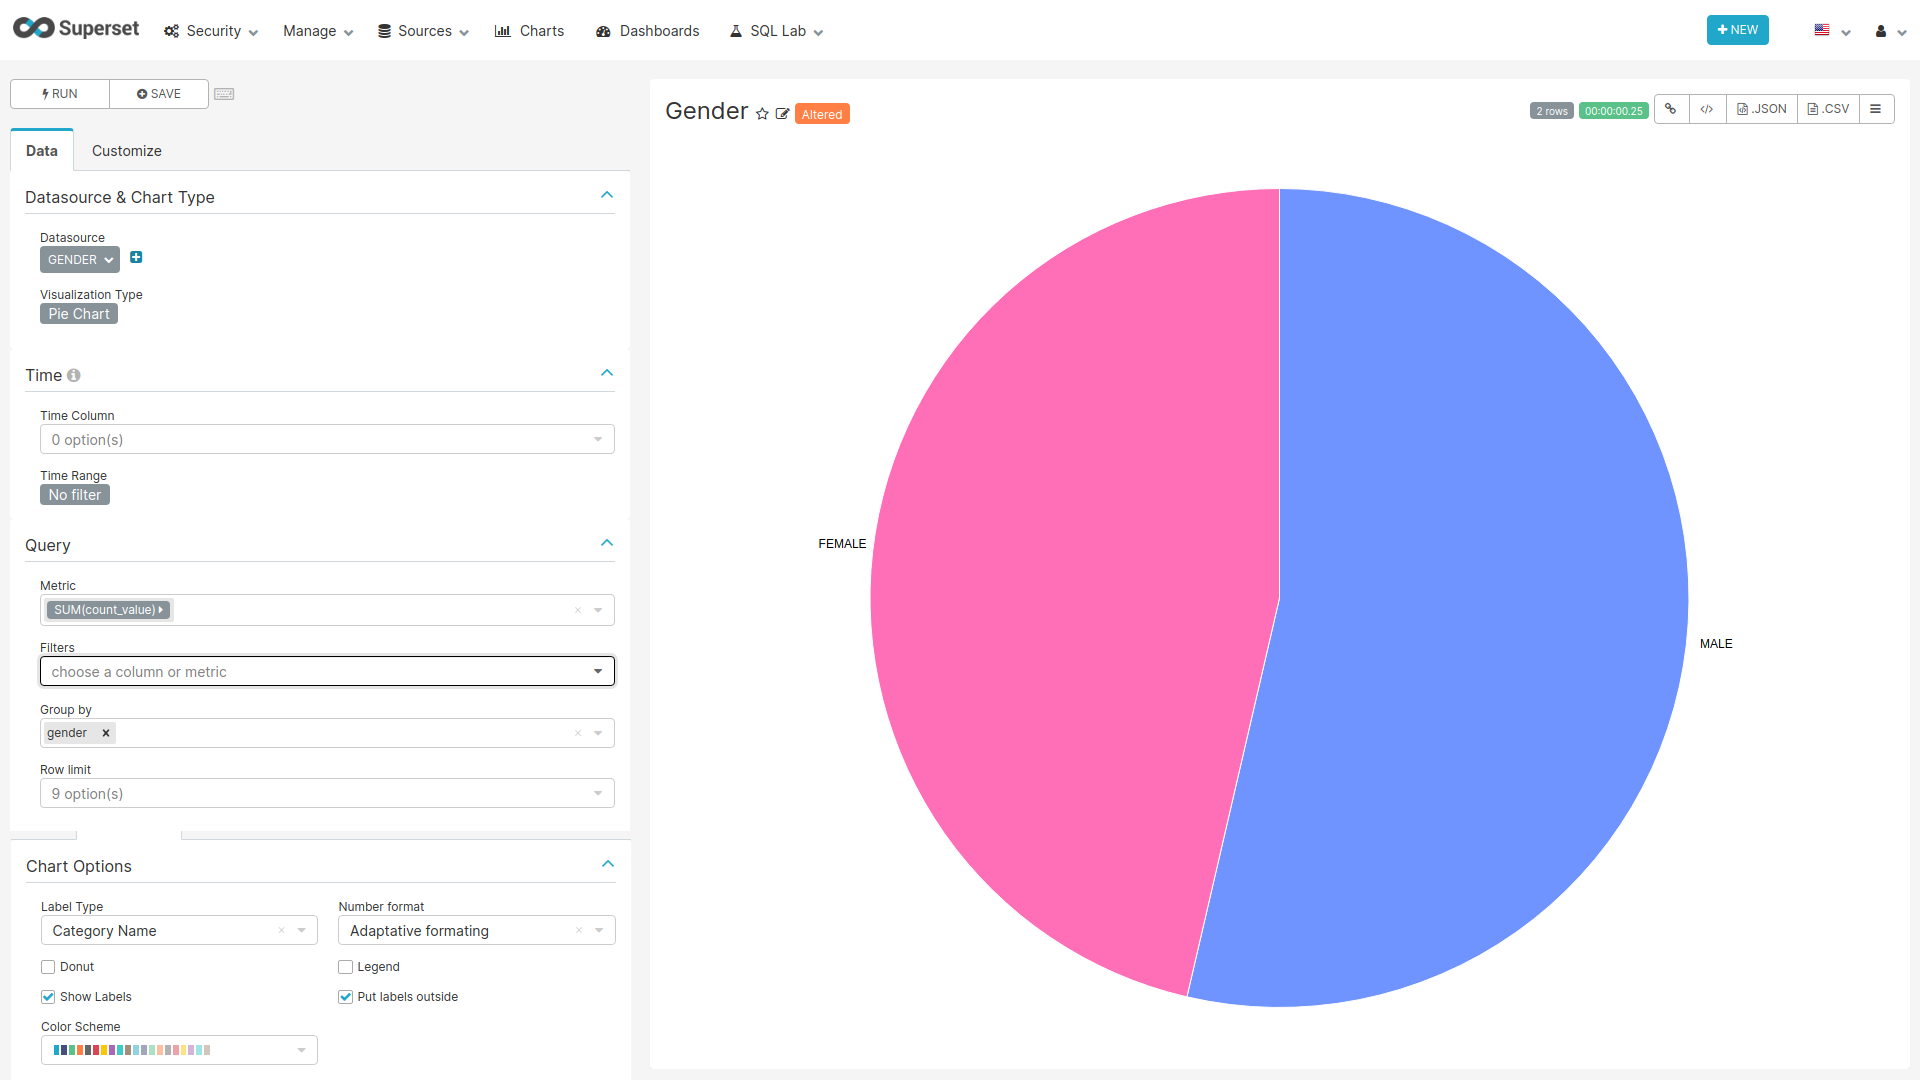
\includegraphics[width=1\linewidth]{images/11-per_database/01-demographics/03-gender_pie} \caption{Settings for creating the Gender Pie chart}\label{fig:genderPie}
\end{figure}

\hypertarget{sql-query-2}{%
\paragraph*{SQL query}\label{sql-query-2}}
\addcontentsline{toc}{paragraph}{SQL query}

Same as \protect\hyperlink{genderTableQuery}{Gender Table} query

\hypertarget{chart-settings-3}{%
\paragraph*{Chart settings}\label{chart-settings-3}}
\addcontentsline{toc}{paragraph}{Chart settings}

\begin{itemize}
\tightlist
\item
  Data Tab

  \begin{itemize}
  \tightlist
  \item
    Datasource \& Chart Type

    \begin{itemize}
    \tightlist
    \item
      Visualization Type: Pie Chart
    \end{itemize}
  \item
    Time

    \begin{itemize}
    \tightlist
    \item
      Time range: No filter
    \end{itemize}
  \item
    Query

    \begin{itemize}
    \tightlist
    \item
      Metric: SUM(count\_value)
    \item
      Group by: gender
    \item
      Row limit: None
    \end{itemize}
  \end{itemize}
\item
  Customize Tab

  \begin{itemize}
  \tightlist
  \item
    Chart Options

    \begin{itemize}
    \tightlist
    \item
      Legend: off
    \end{itemize}
  \end{itemize}
\end{itemize}

\hypertarget{age-at-first-observation---table}{%
\subsubsection*{Age at first observation - Table}\label{age-at-first-observation---table}}
\addcontentsline{toc}{subsubsection}{Age at first observation - Table}

Same chart as the one used on the \protect\hyperlink{age1ObservationTable}{Person} dashboard.

\hypertarget{age-at-first-observation---bars}{%
\subsubsection*{Age at first observation - Bars}\label{age-at-first-observation---bars}}
\addcontentsline{toc}{subsubsection}{Age at first observation - Bars}

Same chart as the one used on the \protect\hyperlink{age1ObservationBars}{Person} dashboard.

\hypertarget{year-of-birth}{%
\subsubsection*{Year of Birth}\label{year-of-birth}}
\addcontentsline{toc}{subsubsection}{Year of Birth}

Same chart as the one used on the \protect\hyperlink{yearOfBirth}{Person} dashboard.

\hypertarget{data-domains-tab}{%
\subsection*{Data Domains Tab}\label{data-domains-tab}}
\addcontentsline{toc}{subsection}{Data Domains Tab}

\hypertarget{average-number-of-records-per-person}{%
\subsubsection*{Average Number of Records per Person}\label{average-number-of-records-per-person}}
\addcontentsline{toc}{subsubsection}{Average Number of Records per Person}

Same chart as the one used on the \protect\hyperlink{avgRecordsPerPerson}{Data Domains} dashboard.

\hypertarget{total-number-of-records}{%
\subsubsection*{Total Number of Records}\label{total-number-of-records}}
\addcontentsline{toc}{subsubsection}{Total Number of Records}

\begin{figure}
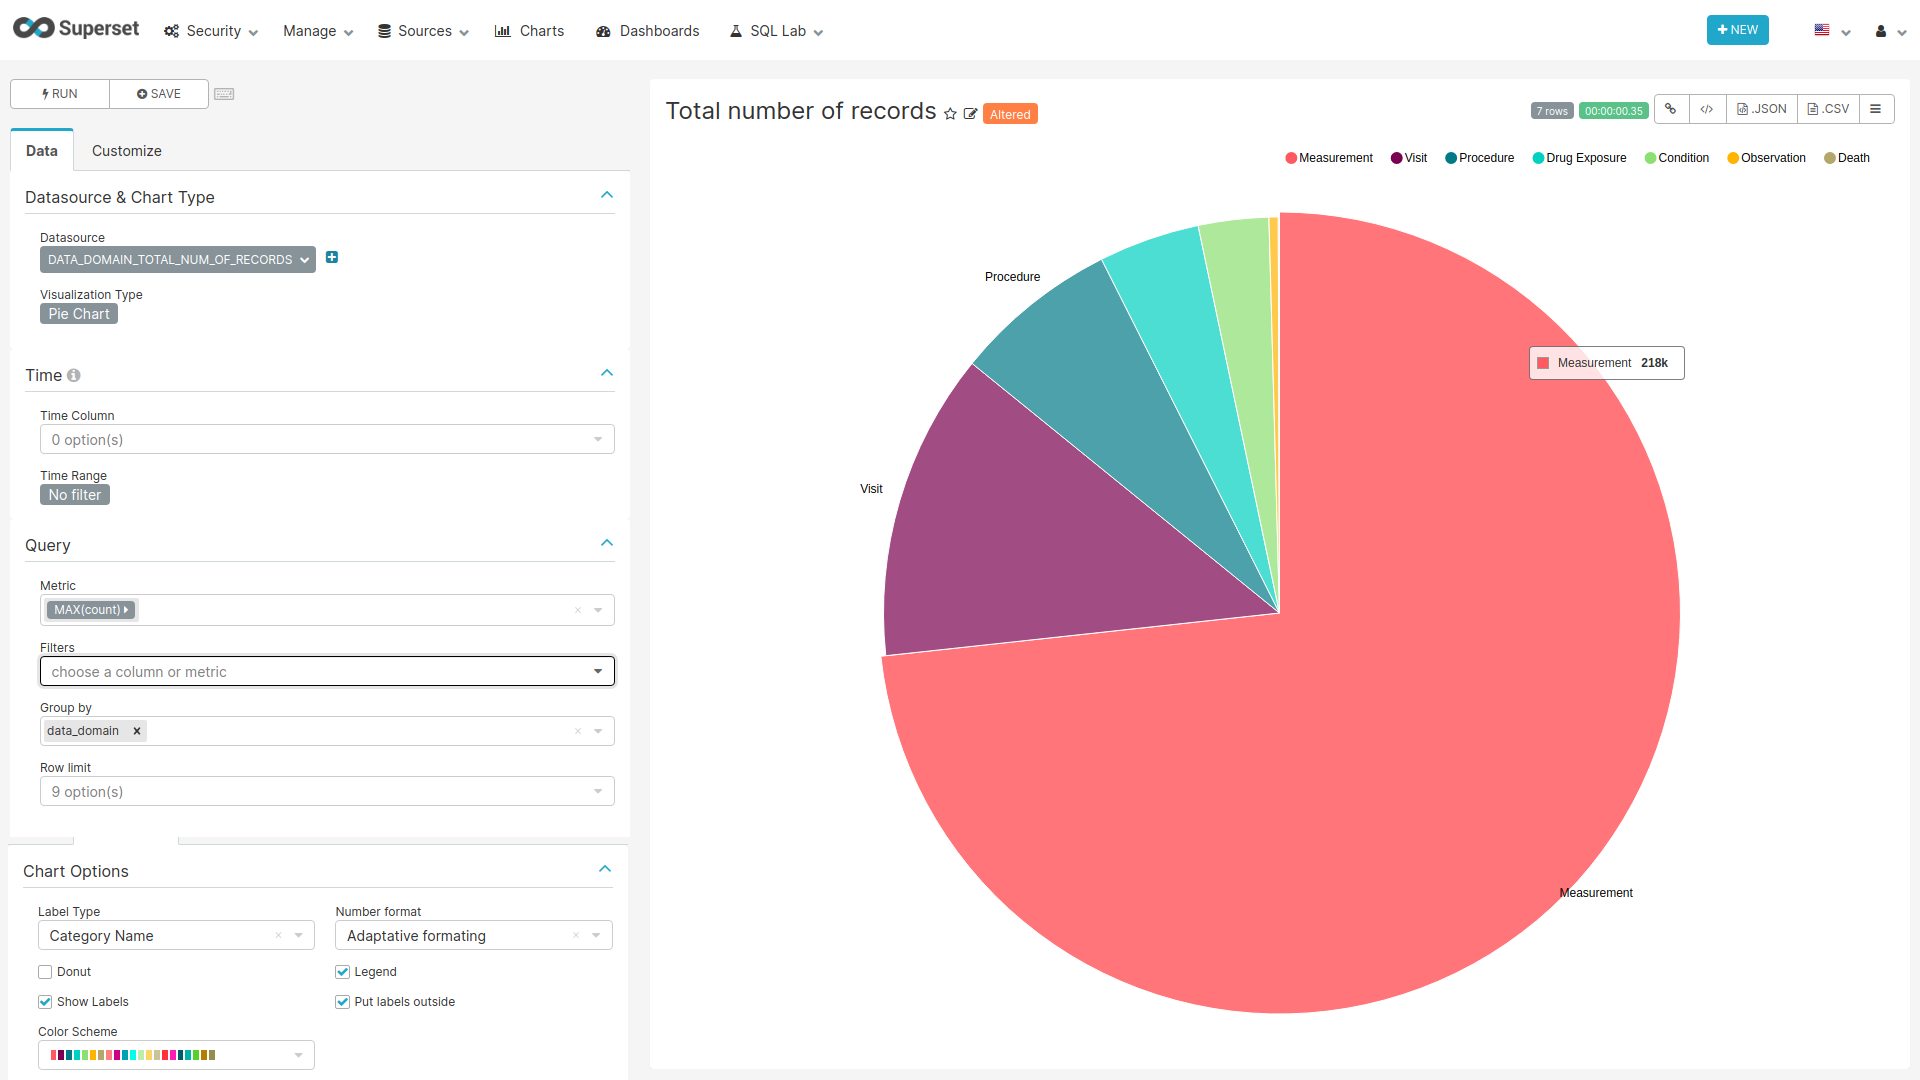
\includegraphics[width=1\linewidth]{images/11-per_database/02-data_domains/02-total_num_records} \caption{Settings for creating the Total Number of Records chart}\label{fig:totalNumRecords}
\end{figure}

\hypertarget{sql-query-3}{%
\paragraph*{SQL query}\label{sql-query-3}}
\addcontentsline{toc}{paragraph}{SQL query}

\begin{Shaded}
\begin{Highlighting}[]
\KeywordTok{SELECT}
\NormalTok{data\_source.name,}
\NormalTok{data\_source.acronym,}
    \ControlFlowTok{CASE} 
    \ControlFlowTok{WHEN}\NormalTok{ analysis\_id }\OperatorTok{=} \DecValTok{201} \ControlFlowTok{THEN} \StringTok{\textquotesingle{}Visit\textquotesingle{}}
    \ControlFlowTok{WHEN}\NormalTok{ analysis\_id }\OperatorTok{=} \DecValTok{401} \ControlFlowTok{THEN} \StringTok{\textquotesingle{}Condition\textquotesingle{}}
    \ControlFlowTok{WHEN}\NormalTok{ analysis\_id }\OperatorTok{=} \DecValTok{501} \ControlFlowTok{THEN} \StringTok{\textquotesingle{}Death\textquotesingle{}}
    \ControlFlowTok{WHEN}\NormalTok{ analysis\_id }\OperatorTok{=} \DecValTok{601} \ControlFlowTok{THEN} \StringTok{\textquotesingle{}Procedure\textquotesingle{}}
    \ControlFlowTok{WHEN}\NormalTok{ analysis\_id }\OperatorTok{=} \DecValTok{701} \ControlFlowTok{THEN} \StringTok{\textquotesingle{}Drug Exposure\textquotesingle{}}
    \ControlFlowTok{WHEN}\NormalTok{ analysis\_id }\OperatorTok{=} \DecValTok{801} \ControlFlowTok{THEN} \StringTok{\textquotesingle{}Observation\textquotesingle{}}
    \ControlFlowTok{WHEN}\NormalTok{ analysis\_id }\OperatorTok{=} \DecValTok{1801} \ControlFlowTok{THEN} \StringTok{\textquotesingle{}Measurement\textquotesingle{}}
    \ControlFlowTok{WHEN}\NormalTok{ analysis\_id }\OperatorTok{=} \DecValTok{2101} \ControlFlowTok{THEN} \StringTok{\textquotesingle{}Device\textquotesingle{}}
    \ControlFlowTok{WHEN}\NormalTok{ analysis\_id }\OperatorTok{=} \DecValTok{2201} \ControlFlowTok{THEN} \StringTok{\textquotesingle{}Note\textquotesingle{}}
    \ControlFlowTok{END} \KeywordTok{AS}\NormalTok{ Data\_Domain,}
    \FunctionTok{SUM}\NormalTok{(count\_value) }\KeywordTok{AS} \OtherTok{"count"}
\KeywordTok{FROM}\NormalTok{ achilles\_results}
\KeywordTok{JOIN}\NormalTok{ data\_source }\KeywordTok{ON}\NormalTok{ achilles\_results.data\_source\_id}\OperatorTok{=}\NormalTok{data\_source.}\KeywordTok{id}
\KeywordTok{GROUP} \KeywordTok{BY}\NormalTok{ name, acronym, analysis\_id}
\KeywordTok{HAVING}\NormalTok{ analysis\_id }\KeywordTok{IN}\NormalTok{ (}\DecValTok{201}\NormalTok{, }\DecValTok{401}\NormalTok{, }\DecValTok{501}\NormalTok{, }\DecValTok{601}\NormalTok{, }\DecValTok{701}\NormalTok{, }\DecValTok{801}\NormalTok{, }\DecValTok{1801}\NormalTok{, }\DecValTok{2101}\NormalTok{, }\DecValTok{2201}\NormalTok{)}
\end{Highlighting}
\end{Shaded}

\hypertarget{chart-settings-4}{%
\paragraph*{Chart settings}\label{chart-settings-4}}
\addcontentsline{toc}{paragraph}{Chart settings}

\begin{itemize}
\tightlist
\item
  Data Tab

  \begin{itemize}
  \tightlist
  \item
    Datasource \& Chart Type

    \begin{itemize}
    \tightlist
    \item
      Visualization Type: Pie Chart
    \end{itemize}
  \item
    Time

    \begin{itemize}
    \tightlist
    \item
      Time range: No filter
    \end{itemize}
  \item
    Query

    \begin{itemize}
    \tightlist
    \item
      Metric: MAX(count)
    \item
      Group by: data\_domain
    \item
      Row limit: None
    \end{itemize}
  \end{itemize}
\end{itemize}

\hypertarget{data-provenance-tab}{%
\subsection*{Data Provenance Tab}\label{data-provenance-tab}}
\addcontentsline{toc}{subsection}{Data Provenance Tab}

Same six charts used on the \protect\hyperlink{dataProvenanceCharts}{Provenance} dashboard.

\hypertarget{observation-period-tab}{%
\subsection*{Observation Period Tab}\label{observation-period-tab}}
\addcontentsline{toc}{subsection}{Observation Period Tab}

\hypertarget{number-of-patitents-in-observation-period}{%
\subsubsection*{Number of Patitents in Observation Period}\label{number-of-patitents-in-observation-period}}
\addcontentsline{toc}{subsubsection}{Number of Patitents in Observation Period}

Same chart used on the \protect\hyperlink{numInObservationPeriod}{Observation Period} dashboard.

\hypertarget{cumulative-observation-period}{%
\subsubsection*{Cumulative Observation Period}\label{cumulative-observation-period}}
\addcontentsline{toc}{subsubsection}{Cumulative Observation Period}

The cumulative observation time plot shows the percentage of patients that have more that X days of observation time.

\begin{figure}
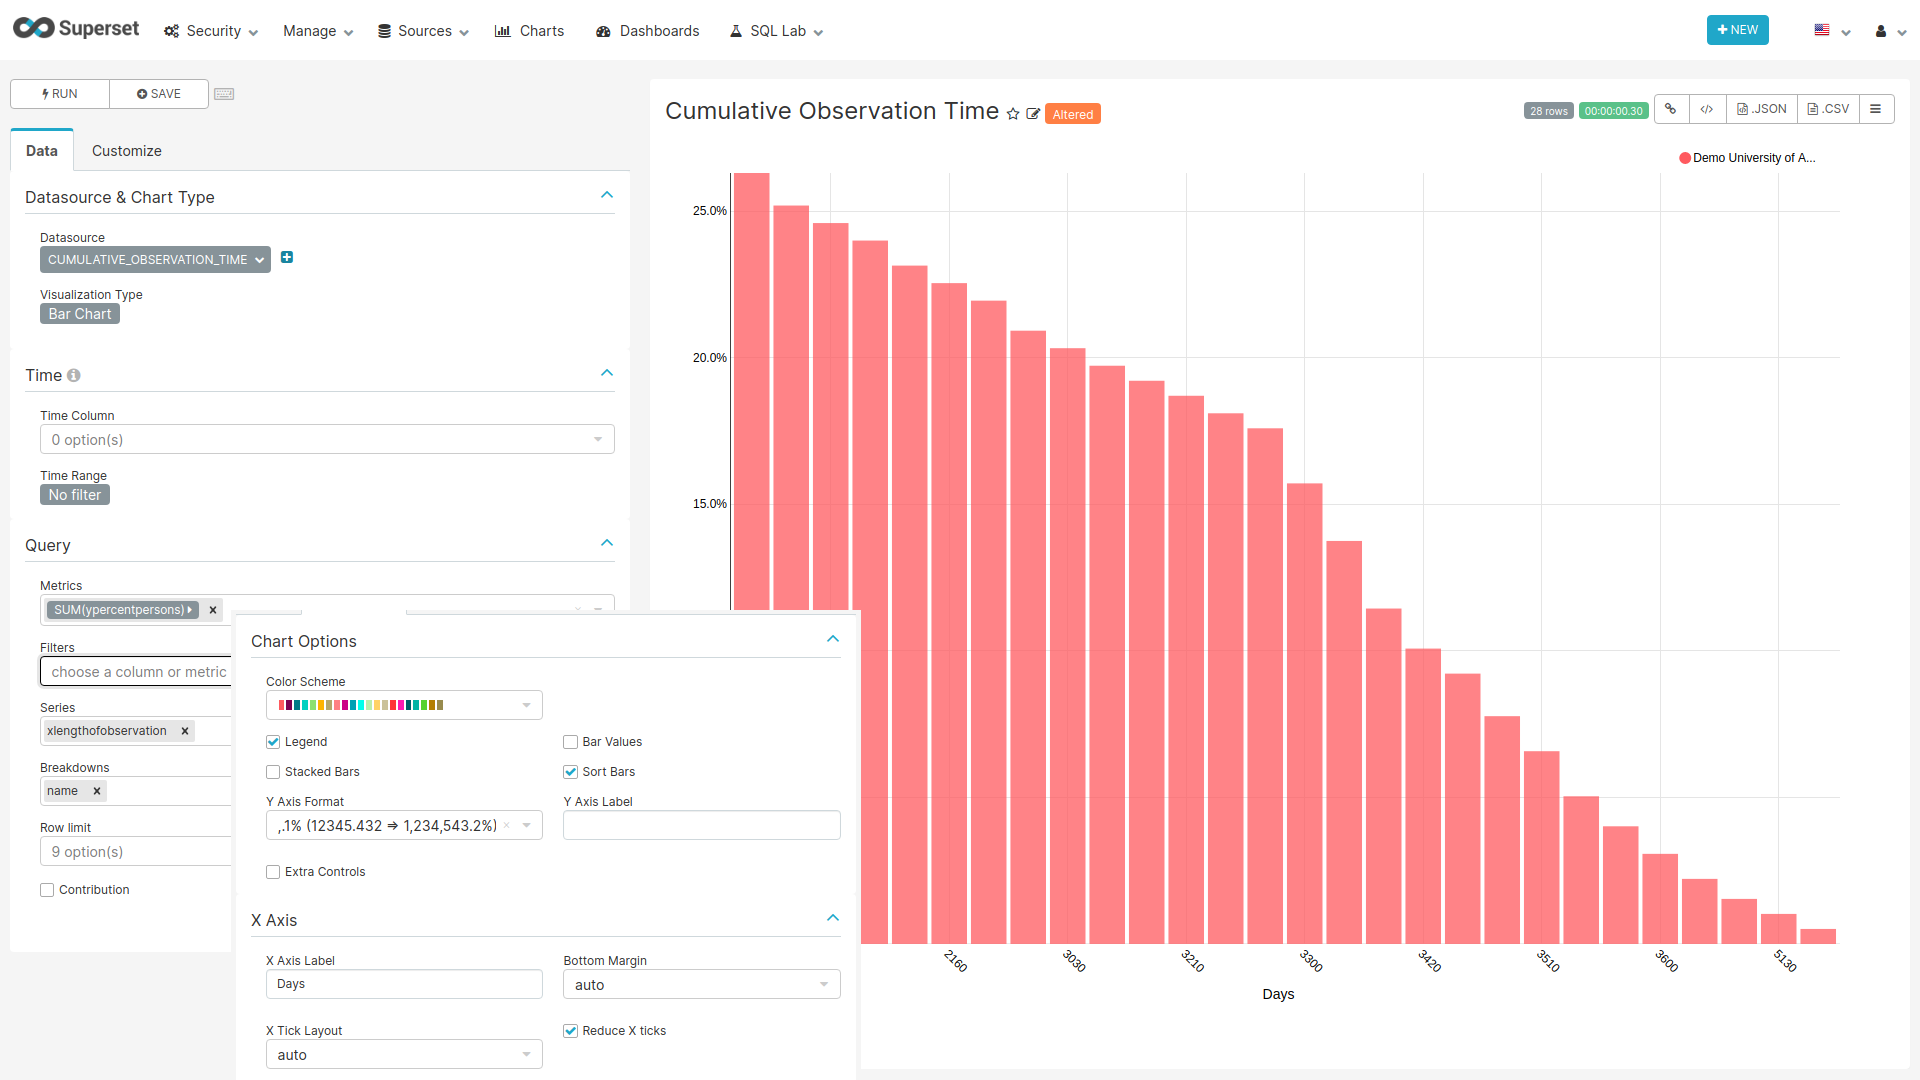
\includegraphics[width=1\linewidth]{images/11-per_database/04-observation_period/02-cum_observation_period} \caption{Settings for creating the Total Number of Records chart}\label{fig:cumObservationTime}
\end{figure}

\hypertarget{sql-query-4}{%
\paragraph*{SQL Query}\label{sql-query-4}}
\addcontentsline{toc}{paragraph}{SQL Query}

\begin{Shaded}
\begin{Highlighting}[]
\KeywordTok{SELECT}
\NormalTok{  name,}
\NormalTok{  acronym,}
\NormalTok{  xLengthOfObservation,}
  \FunctionTok{round}\NormalTok{(cumulative\_sum }\OperatorTok{/}\NormalTok{ total, }\DecValTok{5}\NormalTok{) }\KeywordTok{as}\NormalTok{ yPercentPersons}
\KeywordTok{FROM}\NormalTok{ (}
  \KeywordTok{SELECT}\NormalTok{ data\_source\_id, }\FunctionTok{CAST}\NormalTok{(stratum\_1 }\KeywordTok{AS} \DataTypeTok{INTEGER}\NormalTok{) }\OperatorTok{*} \DecValTok{30} \KeywordTok{AS}\NormalTok{ xLengthOfObservation, }\FunctionTok{SUM}\NormalTok{(count\_value) }\KeywordTok{OVER}\NormalTok{ (}\KeywordTok{PARTITION} \KeywordTok{BY}\NormalTok{ data\_source\_id }\KeywordTok{ORDER} \KeywordTok{BY} \FunctionTok{CAST}\NormalTok{(stratum\_1 }\KeywordTok{AS} \DataTypeTok{INTEGER}\NormalTok{) }\KeywordTok{DESC}\NormalTok{) }\KeywordTok{as}\NormalTok{ cumulative\_sum}
  \KeywordTok{FROM}\NormalTok{ achilles\_results}
  \KeywordTok{WHERE}\NormalTok{ analysis\_id }\OperatorTok{=} \DecValTok{108}
\NormalTok{) }\KeywordTok{AS}\NormalTok{ cumulative\_sums}
\KeywordTok{JOIN}\NormalTok{ (}
  \KeywordTok{SELECT}\NormalTok{ data\_source\_id, count\_value }\KeywordTok{as}\NormalTok{ total}
  \KeywordTok{FROM}\NormalTok{ achilles\_results}
  \KeywordTok{WHERE}\NormalTok{ analysis\_id }\OperatorTok{=} \DecValTok{1}
\NormalTok{) }\KeywordTok{AS}\NormalTok{ totals}
\KeywordTok{ON}\NormalTok{ cumulative\_sums.data\_source\_id }\OperatorTok{=}\NormalTok{ totals.data\_source\_id}
\KeywordTok{JOIN}\NormalTok{ data\_source }\KeywordTok{ON}\NormalTok{ cumulative\_sums.data\_source\_id }\OperatorTok{=}\NormalTok{ data\_source.}\KeywordTok{id}
\KeywordTok{ORDER} \KeywordTok{BY}\NormalTok{ name, xLengthOfObservation}
\end{Highlighting}
\end{Shaded}

\hypertarget{chart-settings-5}{%
\paragraph*{Chart settings}\label{chart-settings-5}}
\addcontentsline{toc}{paragraph}{Chart settings}

\begin{itemize}
\tightlist
\item
  Data Tab

  \begin{itemize}
  \tightlist
  \item
    Datasource \& Chart Type

    \begin{itemize}
    \tightlist
    \item
      Visualization Type: Bar Chart
    \end{itemize}
  \item
    Time

    \begin{itemize}
    \tightlist
    \item
      Time range: No filter
    \end{itemize}
  \item
    Query

    \begin{itemize}
    \tightlist
    \item
      Metrics: SUM(ypercentpersons)
    \item
      Series: xlengthofobservation
    \item
      Breakdowns: name
    \item
      Row limit: None
    \end{itemize}
  \end{itemize}
\item
  Customize Tab

  \begin{itemize}
  \tightlist
  \item
    Chart Options

    \begin{itemize}
    \tightlist
    \item
      Sort Bars: on
    \item
      Y Axis Fomat: ,.1\% (12345.432 =\textgreater{} 1,234,543.2\%)
    \item
      Y Axis Label: Number of Patients
    \end{itemize}
  \item
    X Axis

    \begin{itemize}
    \tightlist
    \item
      X Axis Label: Days
    \item
      Reduce X ticks: on
    \end{itemize}
  \end{itemize}
\end{itemize}

\hypertarget{visit-tab}{%
\subsection*{Visit Tab}\label{visit-tab}}
\addcontentsline{toc}{subsection}{Visit Tab}

\hypertarget{visit-type-graph}{%
\subsubsection*{Visit Type Graph}\label{visit-type-graph}}
\addcontentsline{toc}{subsubsection}{Visit Type Graph}

\begin{figure}
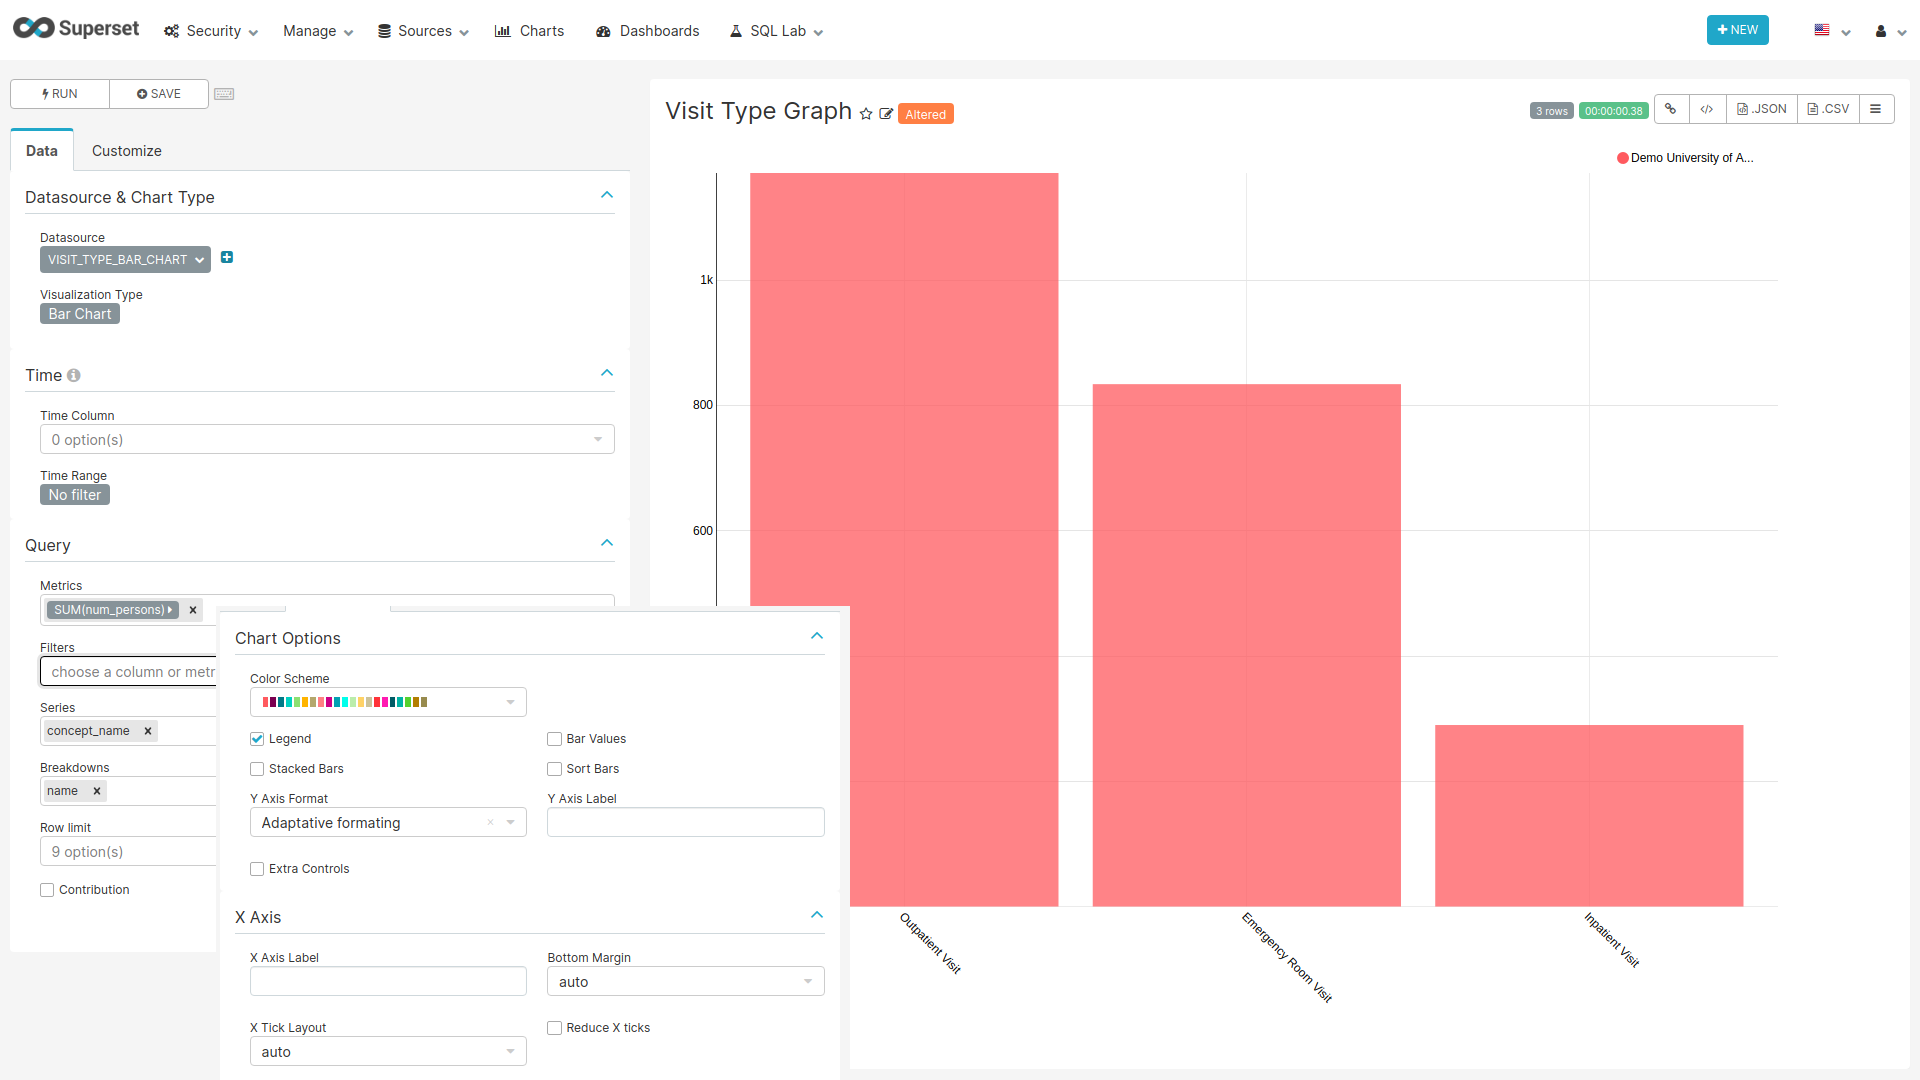
\includegraphics[width=1\linewidth]{images/11-per_database/05-visit/01-visit_type_graph} \caption{Settings for creating the Visit Type Graph chart}\label{fig:visitTypeGraph}
\end{figure}

\hypertarget{sql-query-5}{%
\paragraph*{SQL Query}\label{sql-query-5}}
\addcontentsline{toc}{paragraph}{SQL Query}

\begin{Shaded}
\begin{Highlighting}[]
\KeywordTok{SELECT}
\NormalTok{  data\_source.name,}
\NormalTok{  data\_source.acronym,}
\NormalTok{  concept.concept\_name,}
\NormalTok{  achilles\_results.count\_value }\KeywordTok{AS}\NormalTok{ num\_persons}
\KeywordTok{FROM}\NormalTok{ (}\KeywordTok{SELECT} \OperatorTok{*} \KeywordTok{FROM}\NormalTok{ achilles\_results }\KeywordTok{WHERE}\NormalTok{ analysis\_id }\OperatorTok{=} \DecValTok{200}\NormalTok{) }\KeywordTok{AS}\NormalTok{ achilles\_results}
\KeywordTok{JOIN}\NormalTok{ data\_source }\KeywordTok{ON}\NormalTok{ achilles\_results.data\_source\_id }\OperatorTok{=}\NormalTok{ data\_source.}\KeywordTok{id}
\KeywordTok{JOIN}\NormalTok{ concept }\KeywordTok{ON} \FunctionTok{CAST}\NormalTok{(achilles\_results.stratum\_1 }\KeywordTok{AS}\NormalTok{ BIGINT) }\OperatorTok{=}\NormalTok{ concept.concept\_id}
\end{Highlighting}
\end{Shaded}

\hypertarget{chart-settings-6}{%
\paragraph*{Chart settings}\label{chart-settings-6}}
\addcontentsline{toc}{paragraph}{Chart settings}

\begin{itemize}
\tightlist
\item
  Data Tab

  \begin{itemize}
  \tightlist
  \item
    Datasource \& Chart Type

    \begin{itemize}
    \tightlist
    \item
      Visualization Type: Bar Chart
    \end{itemize}
  \item
    Time

    \begin{itemize}
    \tightlist
    \item
      Time range: No filter
    \end{itemize}
  \item
    Query

    \begin{itemize}
    \tightlist
    \item
      Metrics: SUM(num\_persons)
    \item
      Series: concept\_name
    \item
      Breakdowns: name
    \item
      Row limit: None
    \end{itemize}
  \end{itemize}
\end{itemize}

\hypertarget{visit-type-table}{%
\subsubsection*{Visit Type Table}\label{visit-type-table}}
\addcontentsline{toc}{subsubsection}{Visit Type Table}

\begin{figure}
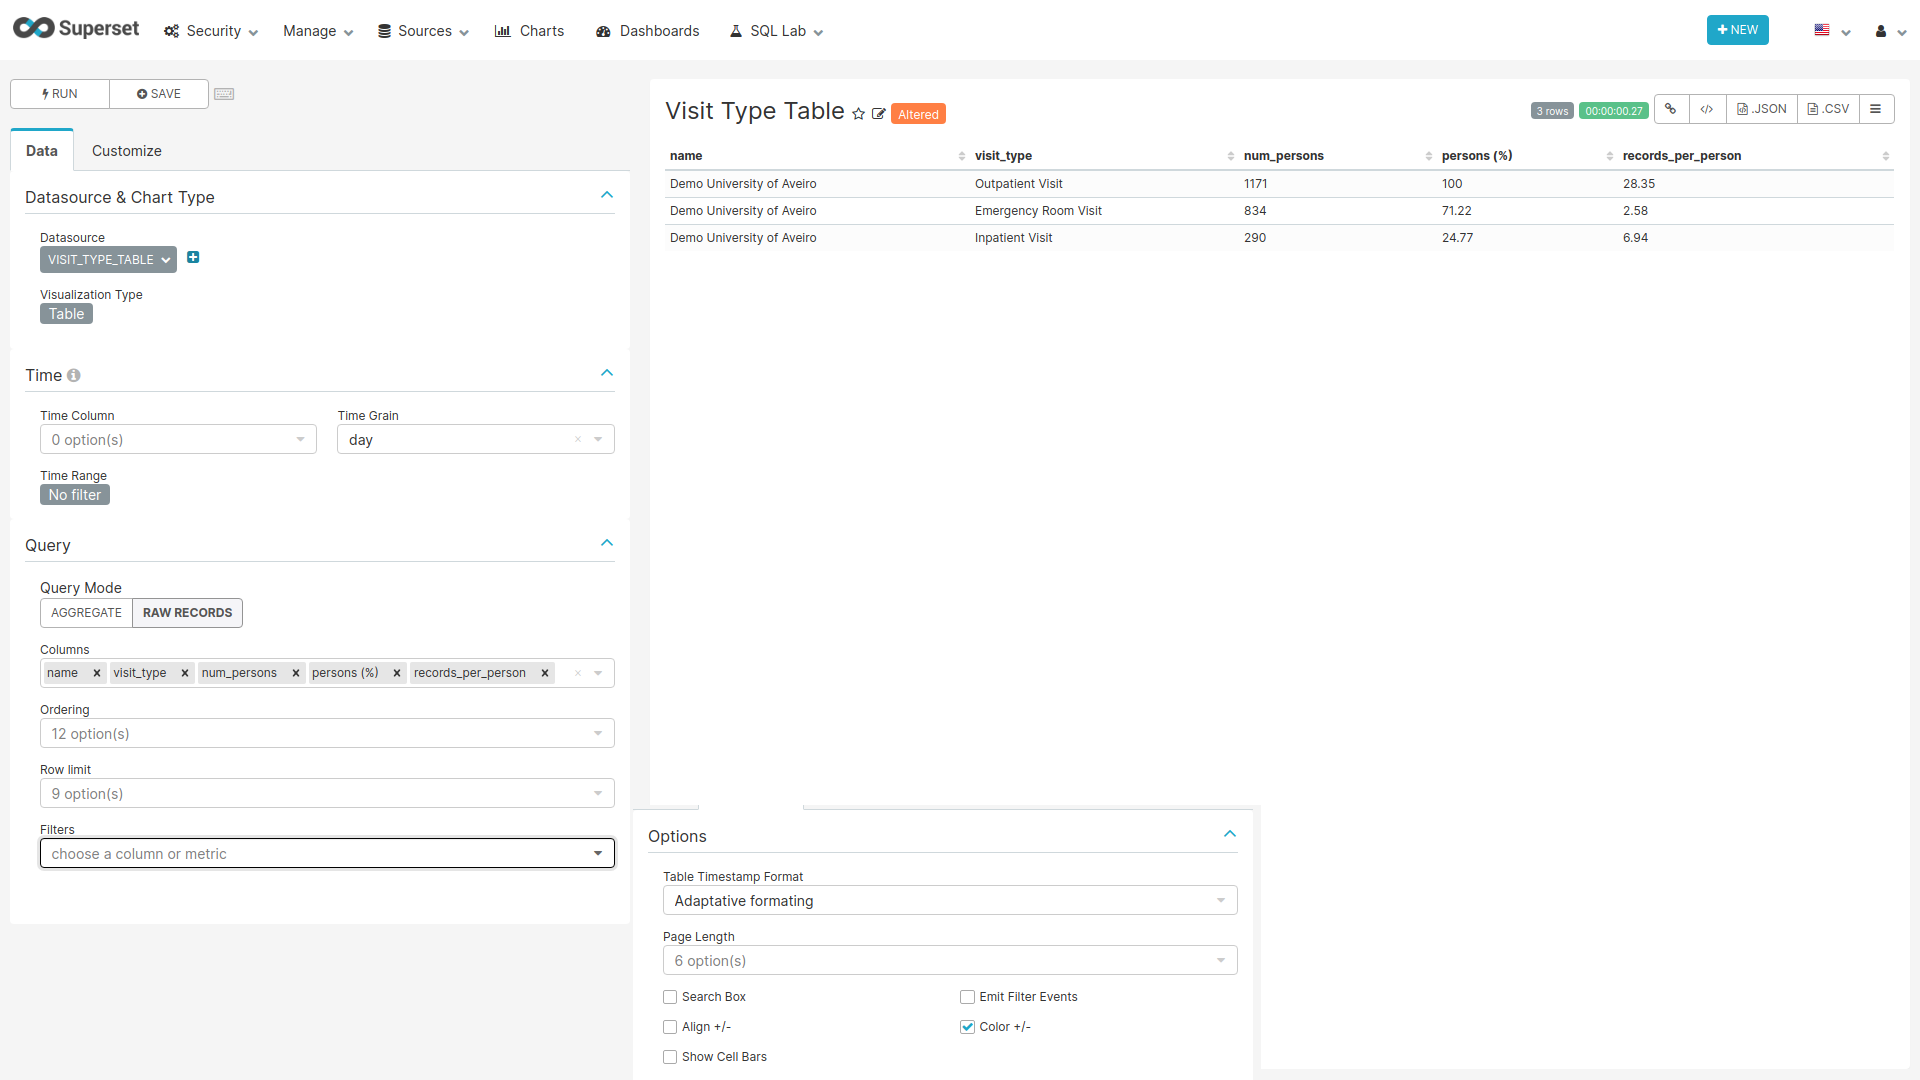
\includegraphics[width=1\linewidth]{images/11-per_database/05-visit/02-visit_type_table} \caption{Settings for creating the Visit Type Table chart}\label{fig:visitTypeTable}
\end{figure}

\hypertarget{sql-query-6}{%
\paragraph*{SQL Query}\label{sql-query-6}}
\addcontentsline{toc}{paragraph}{SQL Query}

\begin{Shaded}
\begin{Highlighting}[]
\KeywordTok{SELECT}
\NormalTok{  name,}
\NormalTok{  acronym,}
\NormalTok{  concept.concept\_name,}
\NormalTok{  ar1.count\_value }\KeywordTok{AS}\NormalTok{ num\_persons,}
  \FunctionTok{round}\NormalTok{(}\FloatTok{100.0} \OperatorTok{*}\NormalTok{ ar1.count\_value }\OperatorTok{/}\NormalTok{ denom.count\_value, }\DecValTok{2}\NormalTok{) }\KeywordTok{AS}\NormalTok{ percent\_persons,}
  \FunctionTok{round}\NormalTok{(}\FloatTok{1.0} \OperatorTok{*}\NormalTok{ ar2.count\_value }\OperatorTok{/}\NormalTok{ ar1.count\_value, }\DecValTok{2}\NormalTok{) }\KeywordTok{AS}\NormalTok{ records\_per\_person}
\KeywordTok{FROM}\NormalTok{ (}
  \KeywordTok{SELECT} \OperatorTok{*}
  \KeywordTok{FROM}\NormalTok{ achilles\_results }\KeywordTok{WHERE}\NormalTok{ analysis\_id }\OperatorTok{=} \DecValTok{200}\NormalTok{) }\KeywordTok{AS}\NormalTok{ ar1}
  \KeywordTok{JOIN}\NormalTok{ (}
    \KeywordTok{SELECT} \OperatorTok{*}
    \KeywordTok{FROM}\NormalTok{ achilles\_results }\KeywordTok{WHERE}\NormalTok{ analysis\_id }\OperatorTok{=} \DecValTok{201}\NormalTok{) }\KeywordTok{AS}\NormalTok{ ar2}
    \KeywordTok{ON}\NormalTok{ ar1.stratum\_1 }\OperatorTok{=}\NormalTok{ ar2.stratum\_1 }\KeywordTok{AND}\NormalTok{ ar1.data\_source\_id }\OperatorTok{=}\NormalTok{ ar2.data\_source\_id}
  \KeywordTok{JOIN}\NormalTok{ (}
    \KeywordTok{SELECT} \OperatorTok{*}
    \KeywordTok{FROM}\NormalTok{ achilles\_results }\KeywordTok{WHERE}\NormalTok{ analysis\_id }\OperatorTok{=} \DecValTok{1}\NormalTok{) }\KeywordTok{AS}\NormalTok{ denom}
    \KeywordTok{ON}\NormalTok{ ar1.data\_source\_id }\OperatorTok{=}\NormalTok{ denom.data\_source\_id}
  \KeywordTok{JOIN}\NormalTok{ data\_source }\KeywordTok{ON}\NormalTok{ data\_source.}\KeywordTok{id} \OperatorTok{=}\NormalTok{ ar1.data\_source\_id}
  \KeywordTok{JOIN}\NormalTok{ concept }\KeywordTok{ON} \FunctionTok{CAST}\NormalTok{(ar1.stratum\_1 }\KeywordTok{AS} \DataTypeTok{INTEGER}\NormalTok{) }\OperatorTok{=}\NormalTok{ concept\_id}
\KeywordTok{ORDER} \KeywordTok{BY}\NormalTok{ ar1.data\_source\_id, ar1.count\_value }\KeywordTok{DESC}
\end{Highlighting}
\end{Shaded}

\hypertarget{chart-settings-7}{%
\paragraph*{Chart Settings}\label{chart-settings-7}}
\addcontentsline{toc}{paragraph}{Chart Settings}

\begin{itemize}
\tightlist
\item
  Data Tab

  \begin{itemize}
  \tightlist
  \item
    Datasource \& Chart Type

    \begin{itemize}
    \tightlist
    \item
      Visualization Type: Table
    \end{itemize}
  \item
    Time

    \begin{itemize}
    \tightlist
    \item
      Time range: No filter
    \end{itemize}
  \item
    Query

    \begin{itemize}
    \tightlist
    \item
      Query Mode: Raw Records
    \item
      Columns: name, visit\_type, num\_persons, percent\_persons with label persons (\%), records\_per\_person
    \item
      Row limit: None
    \end{itemize}
  \end{itemize}
\item
  Customize Tab

  \begin{itemize}
  \tightlist
  \item
    Options

    \begin{itemize}
    \tightlist
    \item
      Show Cell Bars: off
    \end{itemize}
  \end{itemize}
\end{itemize}

\hypertarget{concept-browser-tab}{%
\subsection*{Concept Browser Tab}\label{concept-browser-tab}}
\addcontentsline{toc}{subsection}{Concept Browser Tab}

\hypertarget{concept-browser-table}{%
\subsubsection*{Concept Browser Table}\label{concept-browser-table}}
\addcontentsline{toc}{subsubsection}{Concept Browser Table}

Same chart used on the \protect\hyperlink{conceptBrowserTable}{Concept Browser} dashboard.

\hypertarget{meta-data-tab}{%
\subsection*{Meta Data Tab}\label{meta-data-tab}}
\addcontentsline{toc}{subsection}{Meta Data Tab}

\hypertarget{meta-data-table}{%
\subsubsection*{Meta Data Table}\label{meta-data-table}}
\addcontentsline{toc}{subsubsection}{Meta Data Table}

Same chart used on the \protect\hyperlink{metaDataTable}{General} dashboard.

\hypertarget{database-level-dashboard}{%
\section{Database Level Dashboard}\label{database-level-dashboard}}

This dashboard is an exact copy of the \protect\hyperlink{PerDatabaseDashboard}{Per Database} dashboard but several legends and fields
displayed on the original are hidden either through CSS or by changing some chart settings.
On the following sections we will only present the things to change on the original charts.

\hypertarget{label-colors-1}{%
\subsection*{Label Colors}\label{label-colors-1}}
\addcontentsline{toc}{subsection}{Label Colors}

In order to obtain the colors blue and rose in the chart representing the gender distribution,
add the following JSON entry to the JSON object of the \texttt{JSON\ Metadata} field on the edit dashboard page:

\begin{Shaded}
\begin{Highlighting}[]
\ErrorTok{"label\_colors":} \FunctionTok{\{}
    \DataTypeTok{"Male"}\FunctionTok{:} \StringTok{"\#3366FF"}\FunctionTok{,}
    \DataTypeTok{"Female"}\FunctionTok{:} \StringTok{"\#FF3399"}
\FunctionTok{\}}
\end{Highlighting}
\end{Shaded}

\hypertarget{css-1}{%
\subsection*{CSS}\label{css-1}}
\addcontentsline{toc}{subsection}{CSS}

To hide the dashboard header insert the following css code to the \texttt{CSS} field on the edit page:

\begin{Shaded}
\begin{Highlighting}[]
\CommentTok{/* hides the filter badges on right side of charts */}
\FunctionTok{.dashboard{-}filter{-}indicators{-}container}\NormalTok{ \{}
    \KeywordTok{display}\NormalTok{: }\DecValTok{none}\OperatorTok{;}
\NormalTok{\}}
\CommentTok{/* hides the acronym filter */}
\FunctionTok{.grid{-}content} \OperatorTok{\textgreater{}} \FunctionTok{.dragdroppable.dragdroppable{-}row} \OperatorTok{\textgreater{}} \FunctionTok{.with{-}popover{-}menu}\NormalTok{ \{}
    \KeywordTok{display}\NormalTok{: }\DecValTok{none}\OperatorTok{;}
\NormalTok{\}}
\CommentTok{/*}
\AlertTok{WARNING}\CommentTok{ panel 1 id hardcoded}
\CommentTok{Hides the X Axis Label of the heatmap on the Data Domains tab}
\CommentTok{*/}
\PreprocessorTok{\#TABS{-}nlIU6H5mcT{-}pane{-}1}\NormalTok{ g}\FunctionTok{.x.axis} \OperatorTok{\textgreater{}}\NormalTok{ g}\FunctionTok{.tick}\NormalTok{ text \{}
    \KeywordTok{display}\NormalTok{: }\DecValTok{none}\OperatorTok{;}
\NormalTok{\}}
\CommentTok{/*}
\AlertTok{WARNING}\CommentTok{ panel 2 id hardcoded}
\CommentTok{Hides the X Axis Labels of the bar charts on the Data Provenance tab}
\CommentTok{*/}
\PreprocessorTok{\#TABS{-}nlIU6H5mcT{-}pane{-}2}\NormalTok{ g}\FunctionTok{.nv{-}x.nv{-}axis.nvd3{-}svg} \OperatorTok{\textgreater{}}\NormalTok{ g}\FunctionTok{.nvd3.nv{-}wrap.nv{-}axis} \OperatorTok{\textgreater{}}\NormalTok{ g }\OperatorTok{\textgreater{}}\NormalTok{ g}\FunctionTok{.tick.zero} \OperatorTok{\textgreater{}}\NormalTok{ text \{}
    \KeywordTok{display}\NormalTok{: }\DecValTok{none}\OperatorTok{;}
\NormalTok{\}}
\end{Highlighting}
\end{Shaded}

With this every time you want to edit the dashboard layout you have to either comment the CSS inserted
or remove it so the ``Edit Dashboard'' button can show again.

\hypertarget{data-source-filter---hidden}{%
\subsection*{Data Source Filter - hidden}\label{data-source-filter---hidden}}
\addcontentsline{toc}{subsection}{Data Source Filter - hidden}

\begin{figure}
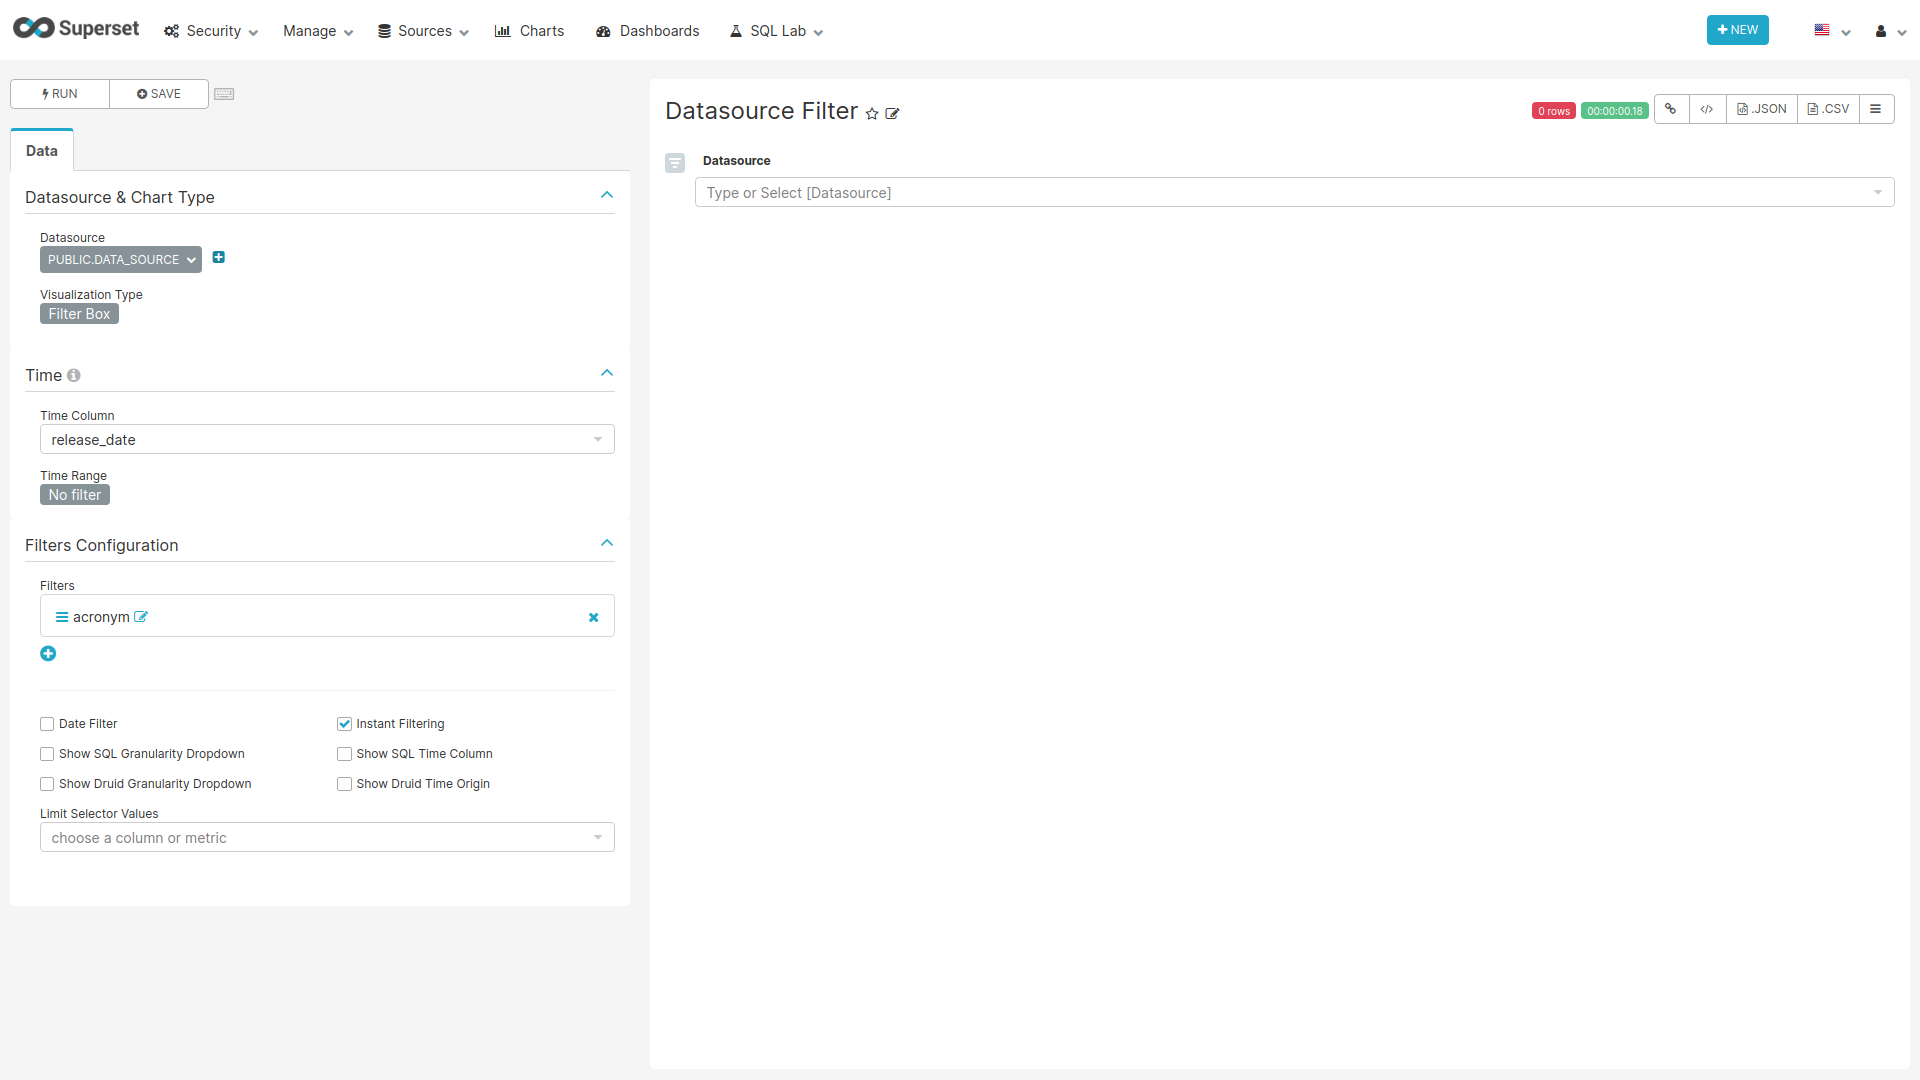
\includegraphics[width=1\linewidth]{images/12-acronym_filter} \caption{Settings for creating the Data Source filter chart}\label{fig:dataSourceFilter}
\end{figure}

\textbf{For the filter to work the name of the fields to filter should match in all tables used on the charts of this dashboard.}

\hypertarget{sql-query-7}{%
\subsubsection*{SQL query}\label{sql-query-7}}
\addcontentsline{toc}{subsubsection}{SQL query}

No SQL query, use the sql table \texttt{data\_source} of the \texttt{achilles} database.

\hypertarget{chart-settings-8}{%
\subsubsection*{Chart settings}\label{chart-settings-8}}
\addcontentsline{toc}{subsubsection}{Chart settings}

\begin{itemize}
\tightlist
\item
  Data Tab

  \begin{itemize}
  \tightlist
  \item
    Datasource \& Chart Type

    \begin{itemize}
    \tightlist
    \item
      Visualization Type: Filter Box
    \end{itemize}
  \item
    Time

    \begin{itemize}
    \tightlist
    \item
      Time range: No filter
    \end{itemize}
  \item
    Filters Configuration

    \begin{itemize}
    \tightlist
    \item
      Filters:

      \begin{itemize}
      \tightlist
      \item
        acronym
      \end{itemize}
    \item
      Date Filter: off
    \item
      Instant Filtering: on
    \end{itemize}
  \end{itemize}
\end{itemize}

\hypertarget{demographics-tab-1}{%
\subsection*{Demographics Tab}\label{demographics-tab-1}}
\addcontentsline{toc}{subsection}{Demographics Tab}

\hypertarget{number-of-patients-1}{%
\subsubsection*{Number of Patients}\label{number-of-patients-1}}
\addcontentsline{toc}{subsubsection}{Number of Patients}

No changes

\hypertarget{gender-table-1}{%
\subsubsection*{Gender Table}\label{gender-table-1}}
\addcontentsline{toc}{subsubsection}{Gender Table}

No changes

\hypertarget{gender-pie-1}{%
\subsubsection*{Gender Pie}\label{gender-pie-1}}
\addcontentsline{toc}{subsubsection}{Gender Pie}

No changes

\hypertarget{age-at-first-observation---table-1}{%
\subsubsection*{Age at first observation - Table}\label{age-at-first-observation---table-1}}
\addcontentsline{toc}{subsubsection}{Age at first observation - Table}

Remove the \texttt{name} field from the columns to display.

\begin{itemize}
\tightlist
\item
  Data Tab

  \begin{itemize}
  \tightlist
  \item
    Query

    \begin{itemize}
    \tightlist
    \item
      Columns: 0-10, 10-20, 20-30, 30-40, 40-50, 50-60, 60-70, 70-80, 80-90, 90+
    \end{itemize}
  \end{itemize}
\end{itemize}

\hypertarget{age-at-first-observation---bars-1}{%
\subsubsection*{Age at first observation - Bars}\label{age-at-first-observation---bars-1}}
\addcontentsline{toc}{subsubsection}{Age at first observation - Bars}

Remove legend.

\begin{itemize}
\tightlist
\item
  Customize Tab

  \begin{itemize}
  \tightlist
  \item
    Chart Options

    \begin{itemize}
    \tightlist
    \item
      Legend: off
    \end{itemize}
  \end{itemize}
\end{itemize}

\hypertarget{year-of-birth-1}{%
\subsubsection*{Year of Birth}\label{year-of-birth-1}}
\addcontentsline{toc}{subsubsection}{Year of Birth}

Remove legend.

\begin{itemize}
\tightlist
\item
  Customize Tab

  \begin{itemize}
  \tightlist
  \item
    Chart Options

    \begin{itemize}
    \tightlist
    \item
      Legend: off
    \end{itemize}
  \end{itemize}
\end{itemize}

\hypertarget{data-domains-tab-1}{%
\subsection*{Data Domains Tab}\label{data-domains-tab-1}}
\addcontentsline{toc}{subsection}{Data Domains Tab}

No changes

\hypertarget{data-provenance-tab-1}{%
\subsection*{Data Provenance Tab}\label{data-provenance-tab-1}}
\addcontentsline{toc}{subsection}{Data Provenance Tab}

No changes

\hypertarget{observation-period-tab-1}{%
\subsection*{Observation Period Tab}\label{observation-period-tab-1}}
\addcontentsline{toc}{subsection}{Observation Period Tab}

\hypertarget{number-of-patitents-in-observation-period-1}{%
\subsubsection*{Number of Patitents in Observation Period}\label{number-of-patitents-in-observation-period-1}}
\addcontentsline{toc}{subsubsection}{Number of Patitents in Observation Period}

Remove legend.

\begin{itemize}
\tightlist
\item
  Customize Tab

  \begin{itemize}
  \tightlist
  \item
    Chart Options

    \begin{itemize}
    \tightlist
    \item
      Legend: off
    \end{itemize}
  \end{itemize}
\end{itemize}

\hypertarget{cumulative-observation-period-1}{%
\subsubsection*{Cumulative Observation Period}\label{cumulative-observation-period-1}}
\addcontentsline{toc}{subsubsection}{Cumulative Observation Period}

Remove legend.

\begin{itemize}
\tightlist
\item
  Customize Tab

  \begin{itemize}
  \tightlist
  \item
    Chart Options

    \begin{itemize}
    \tightlist
    \item
      Legend: off
    \end{itemize}
  \end{itemize}
\end{itemize}

\hypertarget{visit-tab-1}{%
\subsection*{Visit Tab}\label{visit-tab-1}}
\addcontentsline{toc}{subsection}{Visit Tab}

\hypertarget{visit-type-graph-1}{%
\subsubsection*{Visit Type Graph}\label{visit-type-graph-1}}
\addcontentsline{toc}{subsubsection}{Visit Type Graph}

Remove legend.

\begin{itemize}
\tightlist
\item
  Customize Tab

  \begin{itemize}
  \tightlist
  \item
    Chart Options

    \begin{itemize}
    \tightlist
    \item
      Legend: off
    \end{itemize}
  \end{itemize}
\end{itemize}

\hypertarget{visit-type-table-1}{%
\subsubsection*{Visit Type Table}\label{visit-type-table-1}}
\addcontentsline{toc}{subsubsection}{Visit Type Table}

Remove the \texttt{name} field from the columns to display.

\begin{itemize}
\tightlist
\item
  Data Tab

  \begin{itemize}
  \tightlist
  \item
    Query

    \begin{itemize}
    \tightlist
    \item
      Columns: visit\_type, num\_persons, percent\_persons with label persons (\%), records\_per\_person
    \end{itemize}
  \end{itemize}
\end{itemize}

\hypertarget{concept-browser-tab-1}{%
\subsection*{Concept Browser Tab}\label{concept-browser-tab-1}}
\addcontentsline{toc}{subsection}{Concept Browser Tab}

\hypertarget{concept-browser-table-1}{%
\subsubsection*{Concept Browser Table}\label{concept-browser-table-1}}
\addcontentsline{toc}{subsubsection}{Concept Browser Table}

Remove the \texttt{source\_name} field from the columns to display.

\begin{itemize}
\tightlist
\item
  Data Tab

  \begin{itemize}
  \tightlist
  \item
    Query

    \begin{itemize}
    \tightlist
    \item
      Columns: concept\_id, concept\_name, domain\_id, magnitude\_persons, magnitude\_occurrences
    \end{itemize}
  \end{itemize}
\end{itemize}

\hypertarget{meta-data-tab-1}{%
\subsection*{Meta Data Tab}\label{meta-data-tab-1}}
\addcontentsline{toc}{subsection}{Meta Data Tab}

\hypertarget{meta-data-table-1}{%
\subsubsection*{Meta Data Table}\label{meta-data-table-1}}
\addcontentsline{toc}{subsubsection}{Meta Data Table}

Remove the \texttt{name} field from the columns to display.

\begin{itemize}
\tightlist
\item
  Data Tab

  \begin{itemize}
  \tightlist
  \item
    Query

    \begin{itemize}
    \tightlist
    \item
      Columns: source\_release\_date, cdm\_release\_date, cdm\_version, vocabulary\_version
    \end{itemize}
  \end{itemize}
\end{itemize}

\hypertarget{general-deprecated}{%
\section{General {[}Deprecated{]}}\label{general-deprecated}}

\hypertarget{css-2}{%
\subsection*{CSS}\label{css-2}}
\addcontentsline{toc}{subsection}{CSS}

To hide the dashboard header insert the following css code to the \texttt{CSS} field on the edit page:

\begin{Shaded}
\begin{Highlighting}[]
\FunctionTok{.dashboard} \OperatorTok{\textgreater{}}\NormalTok{ div}\InformationTok{:not(}\FunctionTok{.dashboard{-}content}\InformationTok{)}\NormalTok{ \{  }\CommentTok{/* dashboard header */}
  \KeywordTok{display}\NormalTok{: }\DecValTok{none}\OperatorTok{;}
\NormalTok{\}}
\end{Highlighting}
\end{Shaded}

With this every time you want to edit the dashboard layout you have to either comment the CSS inserted
or remove it so the ``Edit Dashboard'' button can show again.

\hypertarget{database-type-and-country-filter}{%
\subsection*{Database Type and Country Filter}\label{database-type-and-country-filter}}
\addcontentsline{toc}{subsection}{Database Type and Country Filter}

\label{fig:filters}Settings for creating filters charts

Theses filter were designed to be used in the dashboard aiming the filtering of the data based on the field `'database\_type'' and ``country'' from the table `'data\_source''.

\textbf{For the filters to work the name of the fields to filter should match in all tables used on the charts of this dashboard.}

\hypertarget{sql-query-8}{%
\subsubsection*{SQL query}\label{sql-query-8}}
\addcontentsline{toc}{subsubsection}{SQL query}

\begin{Shaded}
\begin{Highlighting}[]
\KeywordTok{SELECT} \KeywordTok{source}\NormalTok{.name,}
\NormalTok{       country.country,}
       \KeywordTok{source}\NormalTok{.database\_type,}
       \KeywordTok{source}\NormalTok{.acronym}
\KeywordTok{FROM} \KeywordTok{public}\NormalTok{.data\_source }\KeywordTok{AS} \KeywordTok{source}
\KeywordTok{INNER} \KeywordTok{JOIN} \KeywordTok{public}\NormalTok{.country }\KeywordTok{AS}\NormalTok{ country }\KeywordTok{ON} \KeywordTok{source}\NormalTok{.country\_id}\OperatorTok{=}\NormalTok{country.}\KeywordTok{id}
\end{Highlighting}
\end{Shaded}

\hypertarget{chart-settings-9}{%
\subsubsection*{Chart settings}\label{chart-settings-9}}
\addcontentsline{toc}{subsubsection}{Chart settings}

\begin{itemize}
\tightlist
\item
  Data Tab

  \begin{itemize}
  \tightlist
  \item
    Datasource \& Chart Type

    \begin{itemize}
    \tightlist
    \item
      Visualization Type: Filter Box
    \end{itemize}
  \item
    Time

    \begin{itemize}
    \tightlist
    \item
      Time range: No filter
    \end{itemize}
  \item
    Filters Configuration

    \begin{itemize}
    \tightlist
    \item
      Filters:

      \begin{itemize}
      \tightlist
      \item
        database\_type or country
      \end{itemize}
    \item
      Date Filter: off
    \item
      Instant Filtering: on
    \end{itemize}
  \end{itemize}
\end{itemize}

\hypertarget{total-number-of-patients}{%
\subsection*{Total Number of Patients}\label{total-number-of-patients}}
\addcontentsline{toc}{subsection}{Total Number of Patients}

\label{fig:totalNumberOfPatients}Settings for creating the Total Number of Patients chart

\hypertarget{sql-query-9}{%
\subsubsection*{SQL query}\label{sql-query-9}}
\addcontentsline{toc}{subsubsection}{SQL query}

\begin{Shaded}
\begin{Highlighting}[]
\KeywordTok{SELECT}
\NormalTok{ country,}
\NormalTok{ database\_type,}
\NormalTok{ release\_date,}
 \FunctionTok{SUM}\NormalTok{(count\_value) }\KeywordTok{OVER}\NormalTok{ (}\KeywordTok{ORDER} \KeywordTok{BY}\NormalTok{ release\_date }\KeywordTok{ASC}\NormalTok{)}
\KeywordTok{FROM}\NormalTok{ achilles\_results}
\KeywordTok{JOIN}\NormalTok{ data\_source }\KeywordTok{ON}\NormalTok{ data\_source\_id }\OperatorTok{=}\NormalTok{ data\_source.}\KeywordTok{id}
\KeywordTok{JOIN}\NormalTok{ country }\KeywordTok{ON}\NormalTok{ data\_source.country\_id }\OperatorTok{=}\NormalTok{ country.}\KeywordTok{id}
\KeywordTok{WHERE}\NormalTok{ analysis\_id }\OperatorTok{=} \DecValTok{1}
\end{Highlighting}
\end{Shaded}

\hypertarget{chart-settings-10}{%
\subsubsection*{Chart settings}\label{chart-settings-10}}
\addcontentsline{toc}{subsubsection}{Chart settings}

\begin{itemize}
\tightlist
\item
  Data Tab

  \begin{itemize}
  \tightlist
  \item
    Datasource \& Chart Type

    \begin{itemize}
    \tightlist
    \item
      Visualization Type: Big Number with Trendline
    \end{itemize}
  \item
    Time

    \begin{itemize}
    \tightlist
    \item
      Time range: No filter
    \end{itemize}
  \item
    Query

    \begin{itemize}
    \tightlist
    \item
      Metrics: MAX(sum)
    \item
      Series: release\_date
    \item
      Breakdowns: source
    \end{itemize}
  \end{itemize}
\item
  Customize Tab

  \begin{itemize}
  \tightlist
  \item
    Chart Options

    \begin{itemize}
    \tightlist
    \item
      Big Number Font Size: Small
    \item
      Subheader Font Size: Tiny
    \end{itemize}
  \end{itemize}
\end{itemize}

\hypertarget{network-growth-by-date}{%
\subsection*{Network Growth by Date}\label{network-growth-by-date}}
\addcontentsline{toc}{subsection}{Network Growth by Date}

\label{fig:networkGrowthByDate}Settings for creating the Network Growth by Date chart

\hypertarget{sql-query-10}{%
\subsubsection*{SQL query}\label{sql-query-10}}
\addcontentsline{toc}{subsubsection}{SQL query}

\begin{Shaded}
\begin{Highlighting}[]
\KeywordTok{SELECT}  \KeywordTok{source}\NormalTok{.name }\KeywordTok{AS} \KeywordTok{source}\NormalTok{,}
\NormalTok{        country.country,}
        \KeywordTok{source}\NormalTok{.database\_type,}
        \KeywordTok{source}\NormalTok{.release\_date,}
\NormalTok{        concepts.concept\_name }\KeywordTok{AS}\NormalTok{ gender,}
\NormalTok{        achilles.count\_value }\KeywordTok{as} \FunctionTok{count}
\KeywordTok{FROM} \KeywordTok{public}\NormalTok{.achilles\_results }\KeywordTok{AS}\NormalTok{ achilles}
\KeywordTok{INNER} \KeywordTok{JOIN} \KeywordTok{public}\NormalTok{.data\_source }\KeywordTok{AS} \KeywordTok{source} \KeywordTok{ON}\NormalTok{ achilles.data\_source\_id}\OperatorTok{=}\KeywordTok{source}\NormalTok{.}\KeywordTok{id}
\KeywordTok{INNER} \KeywordTok{JOIN} \KeywordTok{public}\NormalTok{.country }\KeywordTok{AS}\NormalTok{ country }\KeywordTok{ON} \KeywordTok{source}\NormalTok{.country\_id}\OperatorTok{=}\NormalTok{country.}\KeywordTok{id}
\KeywordTok{JOIN}\NormalTok{ (}
  \KeywordTok{SELECT} \StringTok{\textquotesingle{}8507\textquotesingle{}} \KeywordTok{AS}\NormalTok{ concept\_id, }\StringTok{\textquotesingle{}Male\textquotesingle{}} \KeywordTok{AS}\NormalTok{ concept\_name}
  \KeywordTok{UNION}
  \KeywordTok{SELECT} \StringTok{\textquotesingle{}8532\textquotesingle{}}\NormalTok{, }\StringTok{\textquotesingle{}Female\textquotesingle{}}
\NormalTok{) }\KeywordTok{AS}\NormalTok{ concepts }\KeywordTok{ON}\NormalTok{ achilles.stratum\_1 }\OperatorTok{=}\NormalTok{ concept\_id}
\KeywordTok{WHERE}\NormalTok{ analysis\_id }\OperatorTok{=} \DecValTok{2}
\end{Highlighting}
\end{Shaded}

\hypertarget{chart-settings-11}{%
\subsubsection*{Chart settings}\label{chart-settings-11}}
\addcontentsline{toc}{subsubsection}{Chart settings}

\begin{itemize}
\tightlist
\item
  Data Tab

  \begin{itemize}
  \tightlist
  \item
    Datasource \& Chart Type

    \begin{itemize}
    \tightlist
    \item
      Visualization Type: Bar Chart
    \end{itemize}
  \item
    Time

    \begin{itemize}
    \tightlist
    \item
      Time range: No filter
    \end{itemize}
  \item
    Query

    \begin{itemize}
    \tightlist
    \item
      Metrics: SUM(count\_value)
    \item
      Series: release\_date
    \item
      Breakdowns: source
    \end{itemize}
  \end{itemize}
\item
  Customize Tab

  \begin{itemize}
  \tightlist
  \item
    Chart Options

    \begin{itemize}
    \tightlist
    \item
      Stacked Bars: on
    \item
      Sort Bars: on
    \item
      Extra Controls: on
    \end{itemize}
  \item
    X Axis

    \begin{itemize}
    \tightlist
    \item
      Reduce X ticks: on
    \end{itemize}
  \end{itemize}
\end{itemize}

\hypertarget{patients-per-country}{%
\subsection*{Patients per Country}\label{patients-per-country}}
\addcontentsline{toc}{subsection}{Patients per Country}

\label{fig:patientsPerCountry}Settings for creating the Patients per Country chart

\hypertarget{sql-query-patientspercountryquery}{%
\subsubsection*{SQL query \{\#patientsPerCountryQuery\}}\label{sql-query-patientspercountryquery}}
\addcontentsline{toc}{subsubsection}{SQL query \{\#patientsPerCountryQuery\}}

\begin{Shaded}
\begin{Highlighting}[]
\KeywordTok{SELECT}\NormalTok{ country.country,}
       \KeywordTok{source}\NormalTok{.database\_type,}
\NormalTok{       count\_value}
\KeywordTok{FROM} \KeywordTok{public}\NormalTok{.achilles\_results }\KeywordTok{AS}\NormalTok{ achilles }
\KeywordTok{INNER} \KeywordTok{JOIN} \KeywordTok{public}\NormalTok{.data\_source }\KeywordTok{AS} \KeywordTok{source} \KeywordTok{ON}\NormalTok{ achilles.data\_source\_id}\OperatorTok{=}\KeywordTok{source}\NormalTok{.}\KeywordTok{id}
\KeywordTok{INNER} \KeywordTok{JOIN} \KeywordTok{public}\NormalTok{.country }\KeywordTok{AS}\NormalTok{ country }\KeywordTok{ON} \KeywordTok{source}\NormalTok{.country\_id}\OperatorTok{=}\NormalTok{country.}\KeywordTok{id}
\KeywordTok{WHERE}\NormalTok{ analysis\_id }\OperatorTok{=} \DecValTok{1}
\end{Highlighting}
\end{Shaded}

\hypertarget{chart-settings-12}{%
\subsubsection*{Chart settings}\label{chart-settings-12}}
\addcontentsline{toc}{subsubsection}{Chart settings}

\begin{itemize}
\tightlist
\item
  Data Tab

  \begin{itemize}
  \tightlist
  \item
    Datasource \& Chart Type

    \begin{itemize}
    \tightlist
    \item
      Visualization Type: Bar Chart
    \end{itemize}
  \item
    Time

    \begin{itemize}
    \tightlist
    \item
      Time range: No filter
    \end{itemize}
  \item
    Query

    \begin{itemize}
    \tightlist
    \item
      Metrics: SUM(count\_value)
    \item
      Series: country
    \end{itemize}
  \end{itemize}
\item
  Customize Tab

  \begin{itemize}
  \tightlist
  \item
    Chart Options

    \begin{itemize}
    \tightlist
    \item
      Legend: off
    \item
      Y Axis Label: Nº of Patients
    \end{itemize}
  \item
    X Axis

    \begin{itemize}
    \tightlist
    \item
      X Axis Label: Country
    \end{itemize}
  \end{itemize}
\end{itemize}

\hypertarget{database-types-per-country}{%
\subsection*{Database Types per Country}\label{database-types-per-country}}
\addcontentsline{toc}{subsection}{Database Types per Country}

\label{fig:dbsTypesPerCountry}Settings for creating the Database Type per Country chart

\hypertarget{sql-query-11}{%
\subsubsection*{SQL query}\label{sql-query-11}}
\addcontentsline{toc}{subsubsection}{SQL query}

Same as \protect\hyperlink{patientsPerCountryQuery}{Patients per Country} query

\hypertarget{chart-settings-13}{%
\subsubsection*{Chart settings}\label{chart-settings-13}}
\addcontentsline{toc}{subsubsection}{Chart settings}

\begin{itemize}
\tightlist
\item
  Data Tab

  \begin{itemize}
  \tightlist
  \item
    Datasource \& Chart Type

    \begin{itemize}
    \tightlist
    \item
      Visualization Type: Heatmap
    \end{itemize}
  \item
    Time

    \begin{itemize}
    \tightlist
    \item
      Time range: No filter
    \end{itemize}
  \item
    Query

    \begin{itemize}
    \tightlist
    \item
      X: country
    \item
      Y: database\_type
    \item
      Metric: SUM(countr\_value)
    \end{itemize}
  \item
    Heatmap Options

    \begin{itemize}
    \tightlist
    \item
      Left Margin: 75
    \item
      Show Percentage: off
    \end{itemize}
  \end{itemize}
\end{itemize}

\hypertarget{world-map}{%
\subsection*{World Map}\label{world-map}}
\addcontentsline{toc}{subsection}{World Map}

\label{fig:worldMap}Settings for creating the World Map chart

\hypertarget{sql-query-12}{%
\subsubsection*{SQL query}\label{sql-query-12}}
\addcontentsline{toc}{subsubsection}{SQL query}

\begin{Shaded}
\begin{Highlighting}[]
\KeywordTok{SELECT}\NormalTok{  name,}
\NormalTok{        acronym,}
\NormalTok{        database\_type,}
\NormalTok{        latitude,}
\NormalTok{        longitude,}
\NormalTok{        country}
\KeywordTok{FROM} \KeywordTok{public}\NormalTok{.data\_source }\KeywordTok{AS} \KeywordTok{source}
\KeywordTok{INNER} \KeywordTok{JOIN} \KeywordTok{public}\NormalTok{.country }\KeywordTok{AS}\NormalTok{ country }\KeywordTok{ON} \KeywordTok{source}\NormalTok{.country\_id}\OperatorTok{=}\NormalTok{country.}\KeywordTok{id}
\end{Highlighting}
\end{Shaded}

\hypertarget{chart-settings-14}{%
\subsubsection*{Chart settings}\label{chart-settings-14}}
\addcontentsline{toc}{subsubsection}{Chart settings}

\begin{itemize}
\tightlist
\item
  Data Tab

  \begin{itemize}
  \tightlist
  \item
    Datasource \& Chart Type

    \begin{itemize}
    \tightlist
    \item
      Visualization Type: MapBox
    \end{itemize}
  \item
    Time

    \begin{itemize}
    \tightlist
    \item
      Time range: No filter
    \end{itemize}
  \item
    Query

    \begin{itemize}
    \tightlist
    \item
      Longitude: longitude
    \item
      Latitude: latitude
    \end{itemize}
  \item
    Visual Tweaks

    \begin{itemize}
    \tightlist
    \item
      Map Style: Streets or Light or Outdoors
    \end{itemize}
  \end{itemize}
\end{itemize}

\hypertarget{metaDataTable}{%
\subsection*{Meta Data}\label{metaDataTable}}
\addcontentsline{toc}{subsection}{Meta Data}

\label{fig:metaData}Settings for creating the Meta Data chart

\hypertarget{sql-query-13}{%
\subsubsection*{SQL query}\label{sql-query-13}}
\addcontentsline{toc}{subsubsection}{SQL query}

\begin{Shaded}
\begin{Highlighting}[]
\KeywordTok{SELECT}
\NormalTok{  acronym,}
\NormalTok{  stratum\_1 }\KeywordTok{as} \OtherTok{"name"}\NormalTok{,}
\NormalTok{  database\_type,}
\NormalTok{  country,}
\NormalTok{  stratum\_2 }\KeywordTok{as} \OtherTok{"source\_release\_date"}\NormalTok{,}
\NormalTok{  stratum\_3 }\KeywordTok{as} \OtherTok{"cdm\_release\_date"}\NormalTok{,}
\NormalTok{  stratum\_4 }\KeywordTok{as} \OtherTok{"cdm\_version"}\NormalTok{,}
\NormalTok{  stratum\_5 }\KeywordTok{as} \OtherTok{"vocabulary\_version"}
\KeywordTok{FROM}\NormalTok{ achilles\_results}
\KeywordTok{JOIN}\NormalTok{ data\_source }\KeywordTok{ON}\NormalTok{ achilles\_results.data\_source\_id }\OperatorTok{=}\NormalTok{ data\_source.}\KeywordTok{id}
\KeywordTok{JOIN}\NormalTok{ country }\KeywordTok{ON}\NormalTok{ data\_source.country\_id }\OperatorTok{=}\NormalTok{ country.}\KeywordTok{id}
\KeywordTok{WHERE}\NormalTok{ analysis\_id}\OperatorTok{=}\DecValTok{5000}
\end{Highlighting}
\end{Shaded}

\hypertarget{chart-settings-15}{%
\subsubsection*{Chart settings}\label{chart-settings-15}}
\addcontentsline{toc}{subsubsection}{Chart settings}

\begin{itemize}
\tightlist
\item
  Data Tab

  \begin{itemize}
  \tightlist
  \item
    Datasource \& Chart Type

    \begin{itemize}
    \tightlist
    \item
      Visualization Type: Table
    \end{itemize}
  \item
    Time

    \begin{itemize}
    \tightlist
    \item
      Time range: No filter
    \end{itemize}
  \item
    Query

    \begin{itemize}
    \tightlist
    \item
      Query Mode: Raw Records
    \item
      Columns: name, source\_release\_date, cdm\_release\_date, cdm\_version, vocabulary\_version
    \end{itemize}
  \end{itemize}
\end{itemize}

\hypertarget{person-deprecated}{%
\section{Person {[}Deprecated{]}}\label{person-deprecated}}

\hypertarget{label-colors-2}{%
\subsection*{Label Colors}\label{label-colors-2}}
\addcontentsline{toc}{subsection}{Label Colors}

In order to obtain the colors blue and rose in the chart representing the gender distribution,
add the following JSON entry to the JSON object of the \texttt{JSON\ Metadata} field on the edit dashboard page:

\begin{Shaded}
\begin{Highlighting}[]
\ErrorTok{"label\_colors":} \FunctionTok{\{}
    \DataTypeTok{"Male"}\FunctionTok{:} \StringTok{"\#3366FF"}\FunctionTok{,} 
    \DataTypeTok{"Female"}\FunctionTok{:} \StringTok{"\#FF3399"}
\FunctionTok{\}}
\end{Highlighting}
\end{Shaded}

\hypertarget{css-3}{%
\subsection*{CSS}\label{css-3}}
\addcontentsline{toc}{subsection}{CSS}

To hide the dashboard header insert the following css code to the \texttt{CSS} field on the edit page:

\begin{Shaded}
\begin{Highlighting}[]
\FunctionTok{.dashboard} \OperatorTok{\textgreater{}}\NormalTok{ div}\InformationTok{:not(}\FunctionTok{.dashboard{-}content}\InformationTok{)}\NormalTok{ \{  }\CommentTok{/* dashboard header */}
  \KeywordTok{display}\NormalTok{: }\DecValTok{none}\OperatorTok{;}
\NormalTok{\}}
\end{Highlighting}
\end{Shaded}

With this every time you want to edit the dashboard layout you have to either comment the CSS inserted
or remove it so the ``Edit Dashboard'' button can show again.

\hypertarget{data-source-filter-1}{%
\subsection*{Data Source Filter}\label{data-source-filter-1}}
\addcontentsline{toc}{subsection}{Data Source Filter}

\begin{figure}
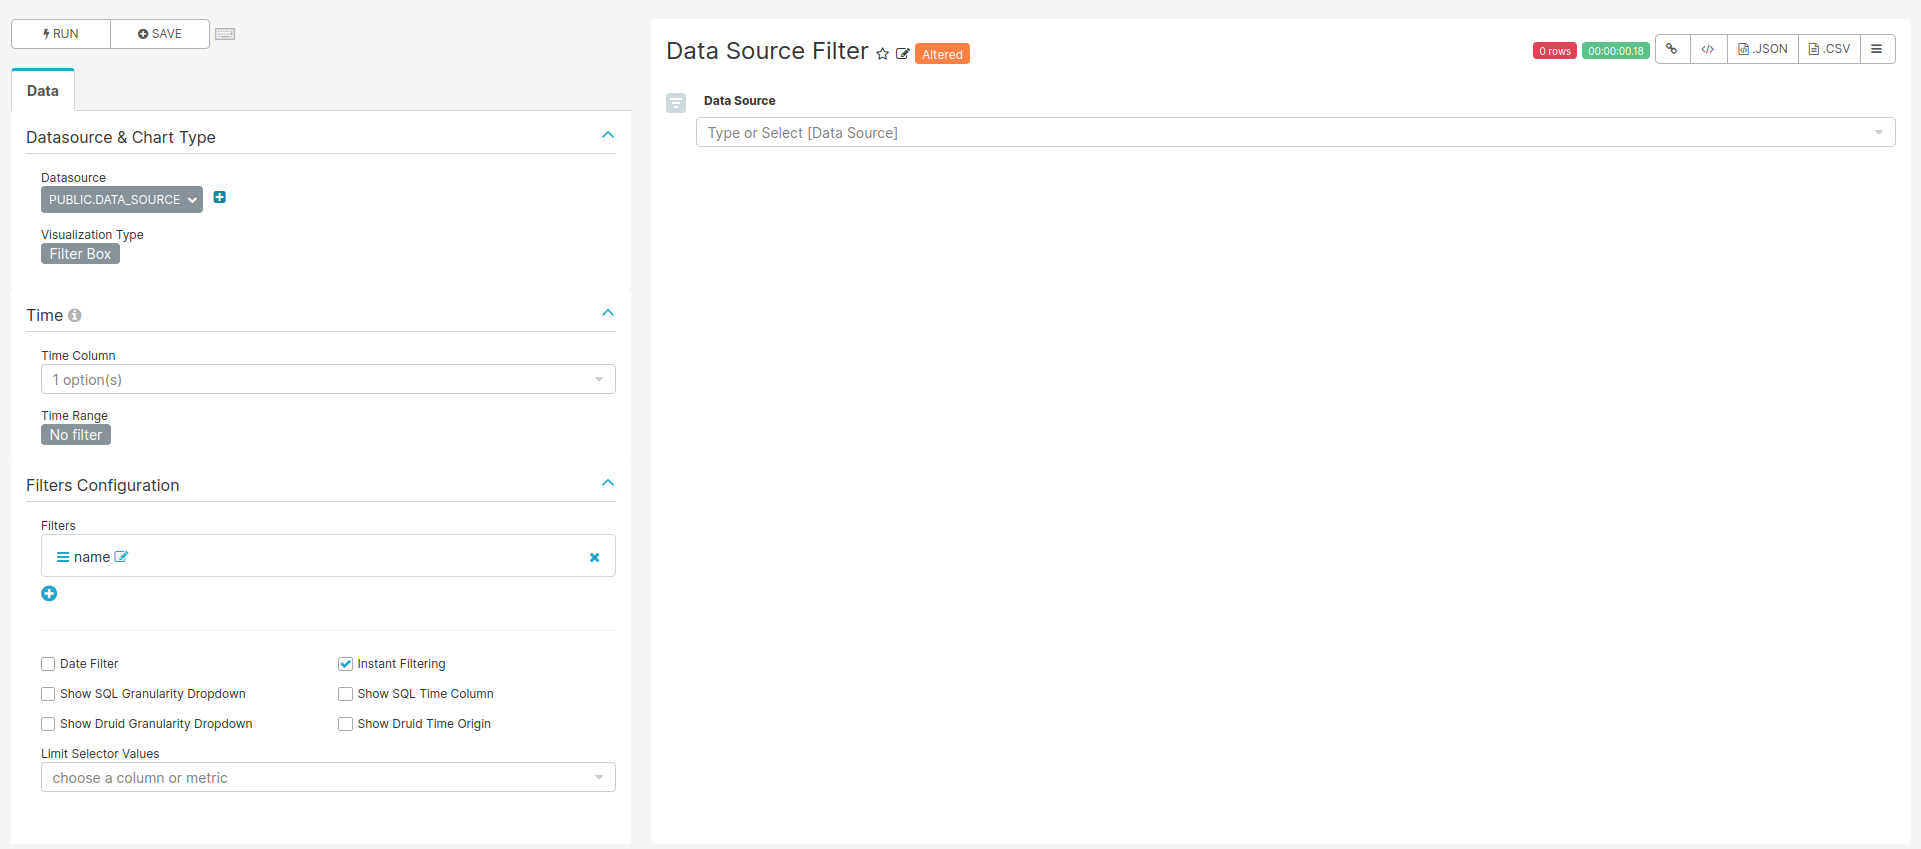
\includegraphics[width=1\linewidth]{images/shared/data_source_filter} \caption{Settings for creating the Data Source filter chart}\label{fig:dataSourceFilter}
\end{figure}

\textbf{For the filter to work the name of the fields to filter should match in all tables used on the charts of this dashboard.}

\hypertarget{sql-query-14}{%
\subsubsection*{SQL query}\label{sql-query-14}}
\addcontentsline{toc}{subsubsection}{SQL query}

No SQL query, use the sql table \texttt{data\_source} of the \texttt{achilles} database.

\hypertarget{chart-settings-16}{%
\subsubsection*{Chart settings}\label{chart-settings-16}}
\addcontentsline{toc}{subsubsection}{Chart settings}

\begin{itemize}
\tightlist
\item
  Data Tab

  \begin{itemize}
  \tightlist
  \item
    Datasource \& Chart Type

    \begin{itemize}
    \tightlist
    \item
      Visualization Type: Filter Box
    \end{itemize}
  \item
    Time

    \begin{itemize}
    \tightlist
    \item
      Time range: No filter
    \end{itemize}
  \item
    Filters Configuration

    \begin{itemize}
    \tightlist
    \item
      Filters:

      \begin{itemize}
      \tightlist
      \item
        name
      \end{itemize}
    \item
      Date Filter: off
    \item
      Instant Filtering: on
    \end{itemize}
  \end{itemize}
\end{itemize}

\hypertarget{age-at-first-observation---table-age1observationtable}{%
\subsection*{Age at first observation - Table \{\#age1ObservationTable\}}\label{age-at-first-observation---table-age1observationtable}}
\addcontentsline{toc}{subsection}{Age at first observation - Table \{\#age1ObservationTable\}}

\begin{figure}
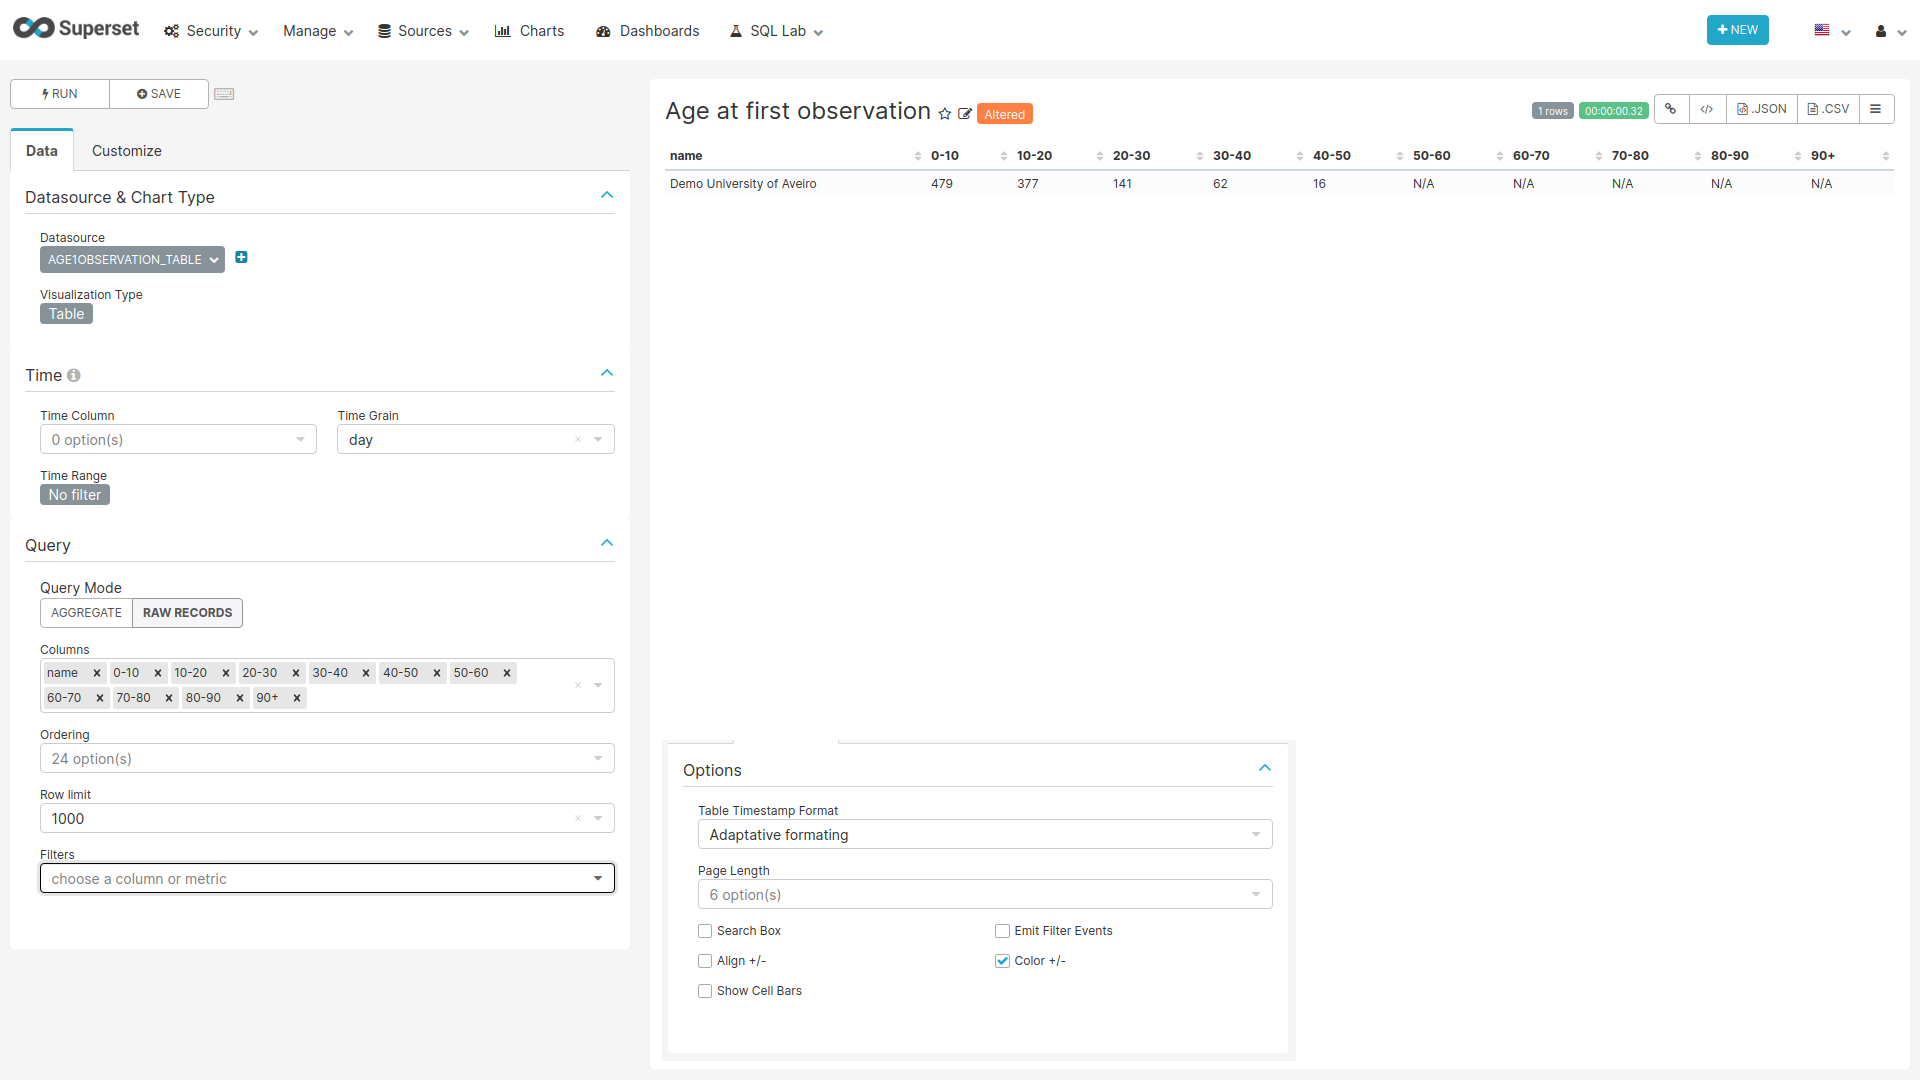
\includegraphics[width=1\linewidth]{images/04-person/02-age_at_first_observation_table} \caption{Settings for creating the Age at First Observation Table chart}\label{fig:ageFirstObservationTable}
\end{figure}

\hypertarget{sql-query-15}{%
\subsubsection*{SQL query}\label{sql-query-15}}
\addcontentsline{toc}{subsubsection}{SQL query}

\begin{Shaded}
\begin{Highlighting}[]
\KeywordTok{SELECT} \KeywordTok{source}\NormalTok{.name,}
       \KeywordTok{source}\NormalTok{.acronym,}
       \FunctionTok{SUM}\NormalTok{(}\ControlFlowTok{CASE} \ControlFlowTok{WHEN} \FunctionTok{CAST}\NormalTok{(stratum\_2 }\KeywordTok{AS} \DataTypeTok{INTEGER}\NormalTok{) }\OperatorTok{\textless{}} \DecValTok{10} \ControlFlowTok{THEN}\NormalTok{ count\_value }\ControlFlowTok{END}\NormalTok{) }\KeywordTok{AS} \OtherTok{"0{-}10"}\NormalTok{,}
       \FunctionTok{SUM}\NormalTok{(}\ControlFlowTok{CASE} \ControlFlowTok{WHEN} \FunctionTok{CAST}\NormalTok{(stratum\_2 }\KeywordTok{AS} \DataTypeTok{INTEGER}\NormalTok{) }\OperatorTok{\textgreater{}=} \DecValTok{10} \KeywordTok{AND} \FunctionTok{CAST}\NormalTok{(stratum\_2 }\KeywordTok{AS} \DataTypeTok{INTEGER}\NormalTok{) }\OperatorTok{\textless{}} \DecValTok{20} \ControlFlowTok{THEN}\NormalTok{ count\_value }\ControlFlowTok{END}\NormalTok{) }\KeywordTok{AS} \OtherTok{"10{-}20"}\NormalTok{,}
       \FunctionTok{SUM}\NormalTok{(}\ControlFlowTok{CASE} \ControlFlowTok{WHEN} \FunctionTok{CAST}\NormalTok{(stratum\_2 }\KeywordTok{AS} \DataTypeTok{INTEGER}\NormalTok{) }\OperatorTok{\textgreater{}=} \DecValTok{20} \KeywordTok{AND} \FunctionTok{CAST}\NormalTok{(stratum\_2 }\KeywordTok{AS} \DataTypeTok{INTEGER}\NormalTok{) }\OperatorTok{\textless{}} \DecValTok{30} \ControlFlowTok{THEN}\NormalTok{ count\_value }\ControlFlowTok{END}\NormalTok{) }\KeywordTok{AS} \OtherTok{"20{-}30"}\NormalTok{,}
       \FunctionTok{SUM}\NormalTok{(}\ControlFlowTok{CASE} \ControlFlowTok{WHEN} \FunctionTok{CAST}\NormalTok{(stratum\_2 }\KeywordTok{AS} \DataTypeTok{INTEGER}\NormalTok{) }\OperatorTok{\textgreater{}=} \DecValTok{30} \KeywordTok{AND} \FunctionTok{CAST}\NormalTok{(stratum\_2 }\KeywordTok{AS} \DataTypeTok{INTEGER}\NormalTok{) }\OperatorTok{\textless{}} \DecValTok{40} \ControlFlowTok{THEN}\NormalTok{ count\_value }\ControlFlowTok{END}\NormalTok{) }\KeywordTok{AS} \OtherTok{"30{-}40"}\NormalTok{,}
       \FunctionTok{SUM}\NormalTok{(}\ControlFlowTok{CASE} \ControlFlowTok{WHEN} \FunctionTok{CAST}\NormalTok{(stratum\_2 }\KeywordTok{AS} \DataTypeTok{INTEGER}\NormalTok{) }\OperatorTok{\textgreater{}=} \DecValTok{40} \KeywordTok{AND} \FunctionTok{CAST}\NormalTok{(stratum\_2 }\KeywordTok{AS} \DataTypeTok{INTEGER}\NormalTok{) }\OperatorTok{\textless{}} \DecValTok{50} \ControlFlowTok{THEN}\NormalTok{ count\_value }\ControlFlowTok{END}\NormalTok{) }\KeywordTok{AS} \OtherTok{"40{-}50"}\NormalTok{,}
       \FunctionTok{SUM}\NormalTok{(}\ControlFlowTok{CASE} \ControlFlowTok{WHEN} \FunctionTok{CAST}\NormalTok{(stratum\_2 }\KeywordTok{AS} \DataTypeTok{INTEGER}\NormalTok{) }\OperatorTok{\textgreater{}=} \DecValTok{50} \KeywordTok{AND} \FunctionTok{CAST}\NormalTok{(stratum\_2 }\KeywordTok{AS} \DataTypeTok{INTEGER}\NormalTok{) }\OperatorTok{\textless{}} \DecValTok{60} \ControlFlowTok{THEN}\NormalTok{ count\_value }\ControlFlowTok{END}\NormalTok{) }\KeywordTok{AS} \OtherTok{"50{-}60"}\NormalTok{,}
       \FunctionTok{SUM}\NormalTok{(}\ControlFlowTok{CASE} \ControlFlowTok{WHEN} \FunctionTok{CAST}\NormalTok{(stratum\_2 }\KeywordTok{AS} \DataTypeTok{INTEGER}\NormalTok{) }\OperatorTok{\textgreater{}=} \DecValTok{60} \KeywordTok{AND} \FunctionTok{CAST}\NormalTok{(stratum\_2 }\KeywordTok{AS} \DataTypeTok{INTEGER}\NormalTok{) }\OperatorTok{\textless{}} \DecValTok{70} \ControlFlowTok{THEN}\NormalTok{ count\_value }\ControlFlowTok{END}\NormalTok{) }\KeywordTok{AS} \OtherTok{"60{-}70"}\NormalTok{,}
       \FunctionTok{SUM}\NormalTok{(}\ControlFlowTok{CASE} \ControlFlowTok{WHEN} \FunctionTok{CAST}\NormalTok{(stratum\_2 }\KeywordTok{AS} \DataTypeTok{INTEGER}\NormalTok{) }\OperatorTok{\textgreater{}=} \DecValTok{70} \KeywordTok{AND} \FunctionTok{CAST}\NormalTok{(stratum\_2 }\KeywordTok{AS} \DataTypeTok{INTEGER}\NormalTok{) }\OperatorTok{\textless{}} \DecValTok{80} \ControlFlowTok{THEN}\NormalTok{ count\_value }\ControlFlowTok{END}\NormalTok{) }\KeywordTok{AS} \OtherTok{"70{-}80"}\NormalTok{,}
       \FunctionTok{SUM}\NormalTok{(}\ControlFlowTok{CASE} \ControlFlowTok{WHEN} \FunctionTok{CAST}\NormalTok{(stratum\_2 }\KeywordTok{AS} \DataTypeTok{INTEGER}\NormalTok{) }\OperatorTok{\textgreater{}=} \DecValTok{80} \KeywordTok{AND} \FunctionTok{CAST}\NormalTok{(stratum\_2 }\KeywordTok{AS} \DataTypeTok{INTEGER}\NormalTok{) }\OperatorTok{\textless{}} \DecValTok{90} \ControlFlowTok{THEN}\NormalTok{ count\_value }\ControlFlowTok{END}\NormalTok{) }\KeywordTok{AS} \OtherTok{"80{-}90"}\NormalTok{,}
       \FunctionTok{SUM}\NormalTok{(}\ControlFlowTok{CASE} \ControlFlowTok{WHEN} \FunctionTok{CAST}\NormalTok{(stratum\_2 }\KeywordTok{AS} \DataTypeTok{INTEGER}\NormalTok{) }\OperatorTok{\textgreater{}=} \DecValTok{90} \ControlFlowTok{THEN}\NormalTok{ count\_value }\ControlFlowTok{END}\NormalTok{) }\KeywordTok{AS} \OtherTok{"90+"}
\KeywordTok{FROM} \KeywordTok{public}\NormalTok{.achilles\_results }\KeywordTok{AS}\NormalTok{ achilles}
\KeywordTok{INNER} \KeywordTok{JOIN} \KeywordTok{public}\NormalTok{.data\_source }\KeywordTok{AS} \KeywordTok{source} \KeywordTok{ON}\NormalTok{ achilles.data\_source\_id}\OperatorTok{=}\KeywordTok{source}\NormalTok{.}\KeywordTok{id}
\KeywordTok{INNER} \KeywordTok{JOIN} \KeywordTok{public}\NormalTok{.concept }\KeywordTok{ON} \FunctionTok{CAST}\NormalTok{(stratum\_1 }\KeywordTok{AS}\NormalTok{ BIGINT) }\OperatorTok{=}\NormalTok{ concept\_id}
\KeywordTok{WHERE}\NormalTok{ analysis\_id }\OperatorTok{=} \DecValTok{102}
\KeywordTok{GROUP} \KeywordTok{BY}\NormalTok{ name, acronym}
\end{Highlighting}
\end{Shaded}

\hypertarget{chart-settings-17}{%
\subsubsection*{Chart settings}\label{chart-settings-17}}
\addcontentsline{toc}{subsubsection}{Chart settings}

\begin{itemize}
\tightlist
\item
  Data Tab

  \begin{itemize}
  \tightlist
  \item
    Datasource \& Chart Type

    \begin{itemize}
    \tightlist
    \item
      Visualization Type: Table
    \end{itemize}
  \item
    Time

    \begin{itemize}
    \tightlist
    \item
      Time range: No filter
    \end{itemize}
  \item
    Query

    \begin{itemize}
    \tightlist
    \item
      Query Mode: Raw Records
    \item
      Columns: name, 0-10, 10-20, 20-30, 30-40, 40-50, 50-60, 60-70, 70-80, 80-90, 90+
    \end{itemize}
  \end{itemize}
\item
  Customize Tab

  \begin{itemize}
  \tightlist
  \item
    Options

    \begin{itemize}
    \tightlist
    \item
      Show Cell Bars: off
    \end{itemize}
  \end{itemize}
\end{itemize}

\hypertarget{age-at-first-observation---bars-age1observationbars}{%
\subsection*{Age at first observation - Bars \{\#age1ObservationBars\}}\label{age-at-first-observation---bars-age1observationbars}}
\addcontentsline{toc}{subsection}{Age at first observation - Bars \{\#age1ObservationBars\}}

\begin{figure}
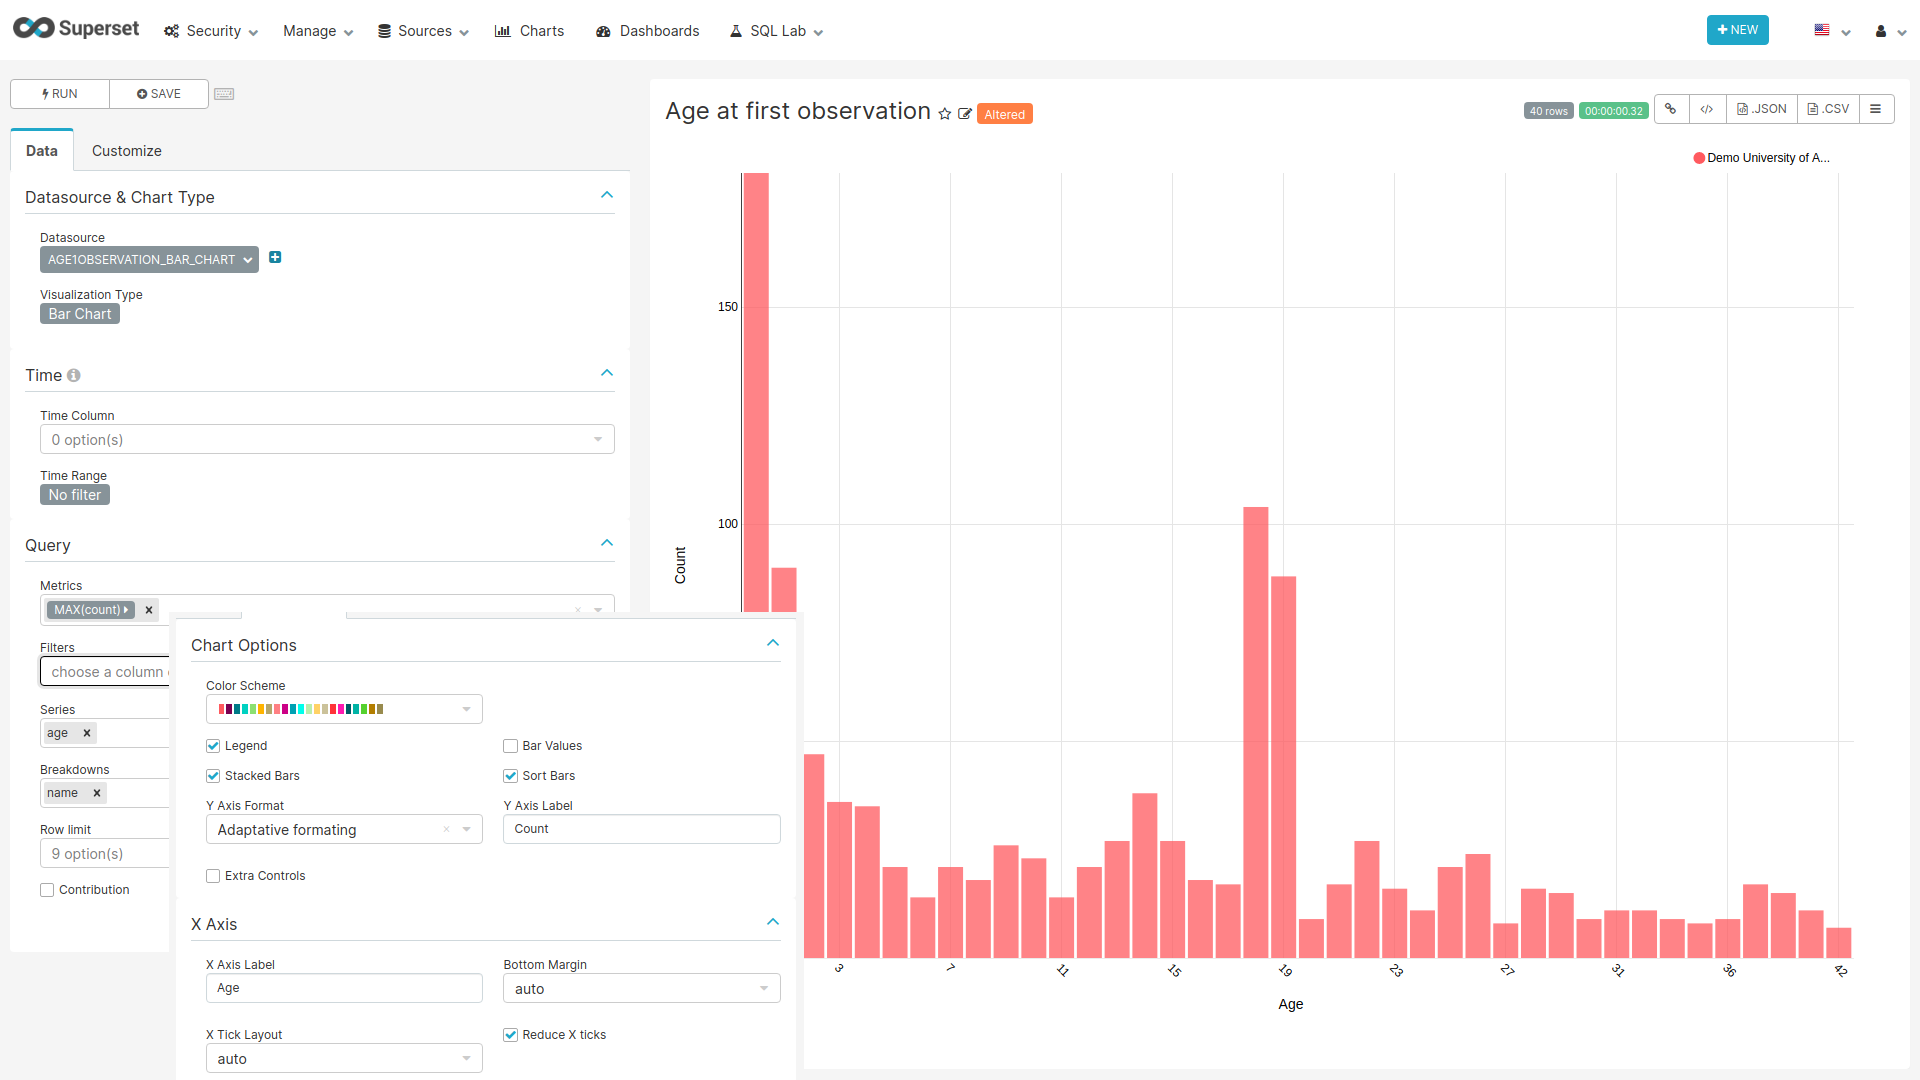
\includegraphics[width=1\linewidth]{images/04-person/03-age_at_first_observation_bar} \caption{Settings for creating the Age at First Observation Bar chart}\label{fig:ageFirstObservationBar}
\end{figure}

\hypertarget{sql-query-16}{%
\subsubsection*{SQL query}\label{sql-query-16}}
\addcontentsline{toc}{subsubsection}{SQL query}

\begin{Shaded}
\begin{Highlighting}[]
\KeywordTok{SELECT} \KeywordTok{source}\NormalTok{.name,}
    \FunctionTok{cast}\NormalTok{(stratum\_1 }\KeywordTok{AS} \DataTypeTok{int}\NormalTok{) }\KeywordTok{AS}\NormalTok{ Age,}
\NormalTok{    count\_value }\KeywordTok{AS} \FunctionTok{count}\NormalTok{, }
    \KeywordTok{source}\NormalTok{.acronym}
\KeywordTok{FROM} \KeywordTok{public}\NormalTok{.achilles\_results }\KeywordTok{AS}\NormalTok{ achilles}
\KeywordTok{INNER} \KeywordTok{JOIN} \KeywordTok{public}\NormalTok{.data\_source }\KeywordTok{AS} \KeywordTok{source} \KeywordTok{ON}\NormalTok{ achilles.data\_source\_id}\OperatorTok{=}\KeywordTok{source}\NormalTok{.}\KeywordTok{id}
\KeywordTok{WHERE}\NormalTok{ analysis\_id }\OperatorTok{=} \DecValTok{101}
\end{Highlighting}
\end{Shaded}

\hypertarget{chart-settings-18}{%
\subsubsection*{Chart settings}\label{chart-settings-18}}
\addcontentsline{toc}{subsubsection}{Chart settings}

\begin{itemize}
\tightlist
\item
  Data Tab

  \begin{itemize}
  \tightlist
  \item
    Datasource \& Chart Type

    \begin{itemize}
    \tightlist
    \item
      Visualization Type: Bar Chart
    \end{itemize}
  \item
    Time

    \begin{itemize}
    \tightlist
    \item
      Time range: No filter
    \end{itemize}
  \item
    Query

    \begin{itemize}
    \tightlist
    \item
      Metrics: MAX(count)
    \item
      Series: age
    \item
      Breakdowns: name
    \end{itemize}
  \end{itemize}
\item
  Customize Tab

  \begin{itemize}
  \tightlist
  \item
    Chart Options

    \begin{itemize}
    \tightlist
    \item
      Stacked Bars: on
    \item
      Sort Bars: on
    \item
      Y Axis Label: Count
    \end{itemize}
  \item
    X Axis

    \begin{itemize}
    \tightlist
    \item
      X Axis Label: Age
    \item
      Reduce X ticks: on
    \end{itemize}
  \end{itemize}
\end{itemize}

\hypertarget{year-of-birth-yearofbirth}{%
\subsection*{Year of Birth \{\#yearOfBirth\}}\label{year-of-birth-yearofbirth}}
\addcontentsline{toc}{subsection}{Year of Birth \{\#yearOfBirth\}}

\begin{figure}
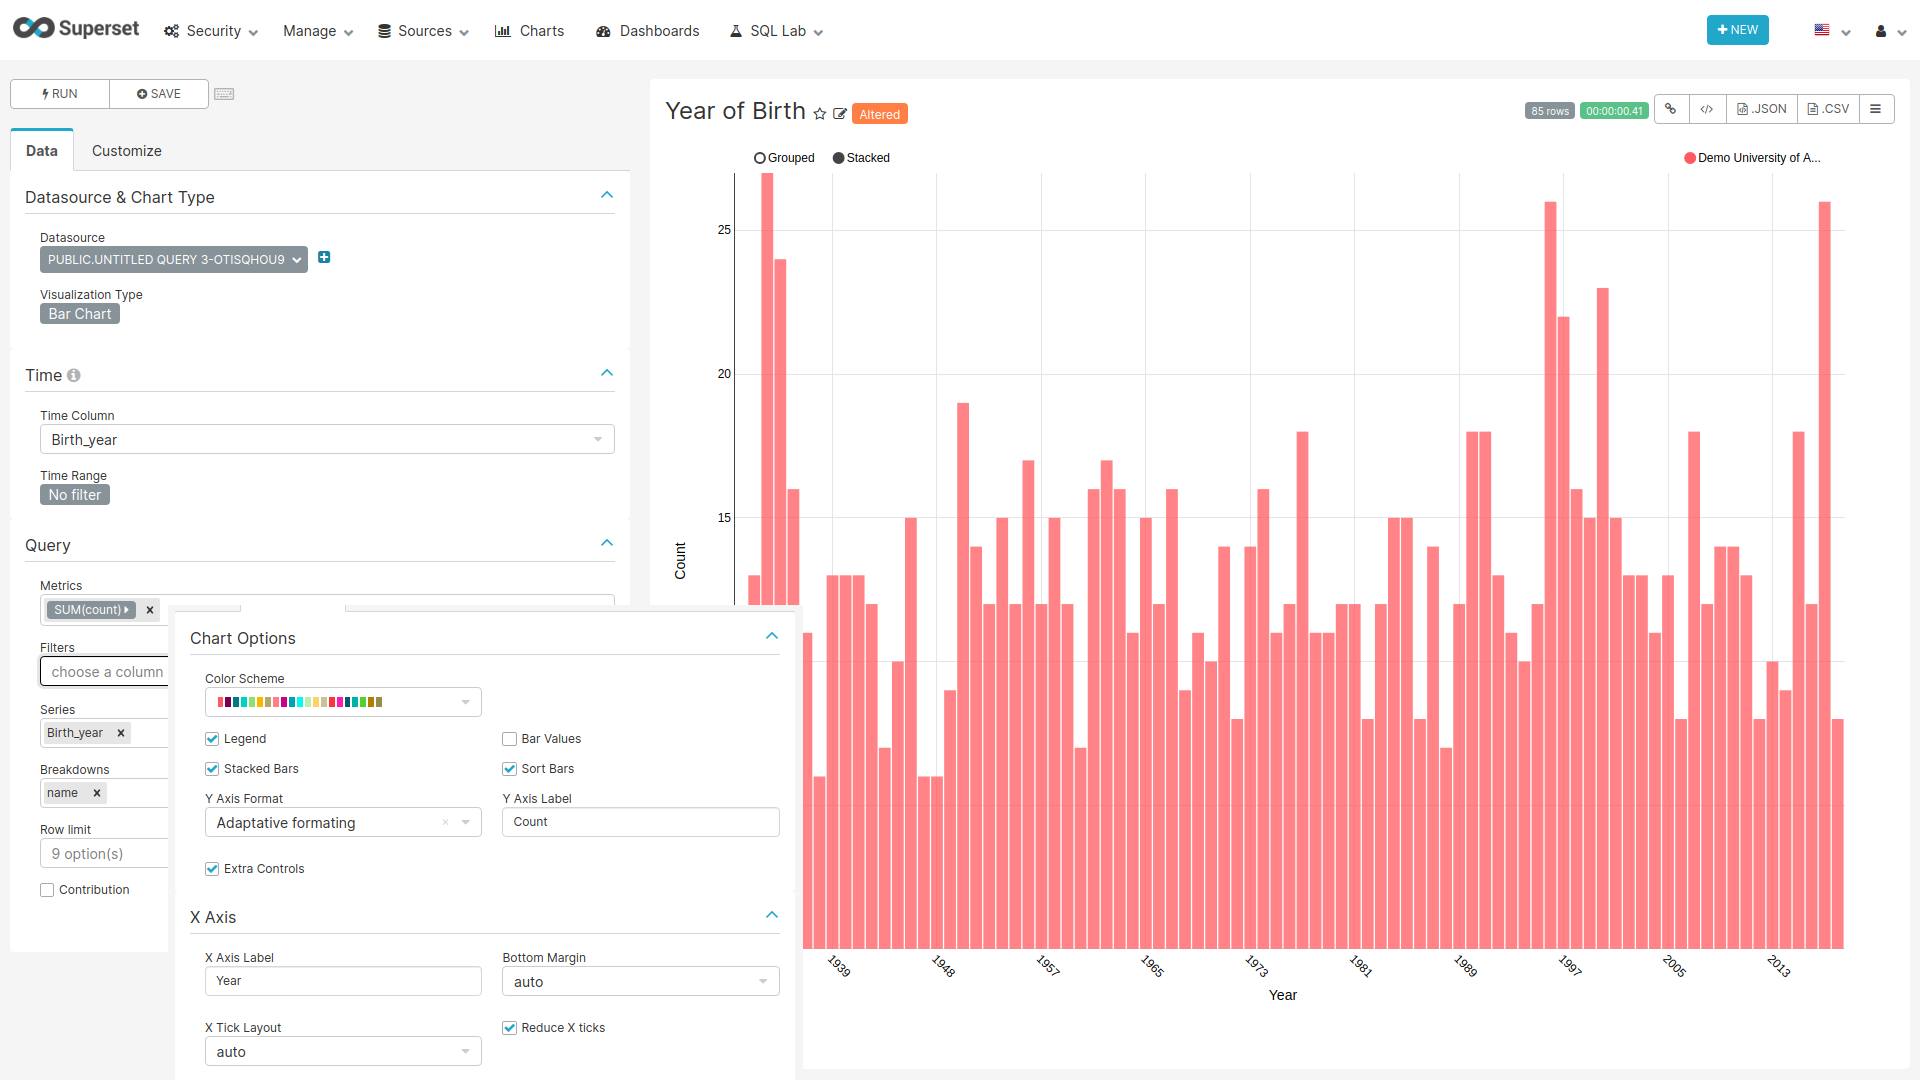
\includegraphics[width=1\linewidth]{images/04-person/04-year_of_birth} \caption{Settings for creating the Year of Birth chart}\label{fig:yearOfBirth}
\end{figure}

\hypertarget{sql-query-17}{%
\subsubsection*{SQL query}\label{sql-query-17}}
\addcontentsline{toc}{subsubsection}{SQL query}

\begin{Shaded}
\begin{Highlighting}[]
\KeywordTok{SELECT} \KeywordTok{source}\NormalTok{.name,}
       \KeywordTok{source}\NormalTok{.acronym,}
\NormalTok{       stratum\_1 }\KeywordTok{AS} \OtherTok{"Birth\_year"}\NormalTok{,}
\NormalTok{       count\_value }\KeywordTok{AS} \FunctionTok{count}
\KeywordTok{FROM} \KeywordTok{public}\NormalTok{.achilles\_results }\KeywordTok{AS}\NormalTok{ achilles}
\KeywordTok{INNER} \KeywordTok{JOIN} \KeywordTok{public}\NormalTok{.data\_source }\KeywordTok{AS} \KeywordTok{source} \KeywordTok{ON}\NormalTok{ achilles.data\_source\_id}\OperatorTok{=}\KeywordTok{source}\NormalTok{.}\KeywordTok{id}
\KeywordTok{WHERE}\NormalTok{ analysis\_id }\OperatorTok{=} \DecValTok{3}
\end{Highlighting}
\end{Shaded}

\hypertarget{chart-settings-19}{%
\subsubsection*{Chart settings}\label{chart-settings-19}}
\addcontentsline{toc}{subsubsection}{Chart settings}

\begin{itemize}
\tightlist
\item
  Data Tab

  \begin{itemize}
  \tightlist
  \item
    Datasource \& Chart Type

    \begin{itemize}
    \tightlist
    \item
      Visualization Type: Bar Chart
    \end{itemize}
  \item
    Time

    \begin{itemize}
    \tightlist
    \item
      Time range: No filter
    \end{itemize}
  \item
    Query

    \begin{itemize}
    \tightlist
    \item
      Metrics: SUM(count)
    \item
      Series: Birth\_year
    \item
      Breakdowns: name
    \end{itemize}
  \end{itemize}
\item
  Customize Tab

  \begin{itemize}
  \tightlist
  \item
    Chart Options

    \begin{itemize}
    \tightlist
    \item
      Stacked Bars: on
    \item
      Sort Bars: on
    \item
      Y Axis Label: Count
    \item
      Extra Controls: on
    \end{itemize}
  \item
    X Axis

    \begin{itemize}
    \tightlist
    \item
      X Axis Label: Year
    \item
      Reduce X ticks: on
    \end{itemize}
  \end{itemize}
\end{itemize}

\hypertarget{gender}{%
\subsection*{Gender}\label{gender}}
\addcontentsline{toc}{subsection}{Gender}

\begin{figure}
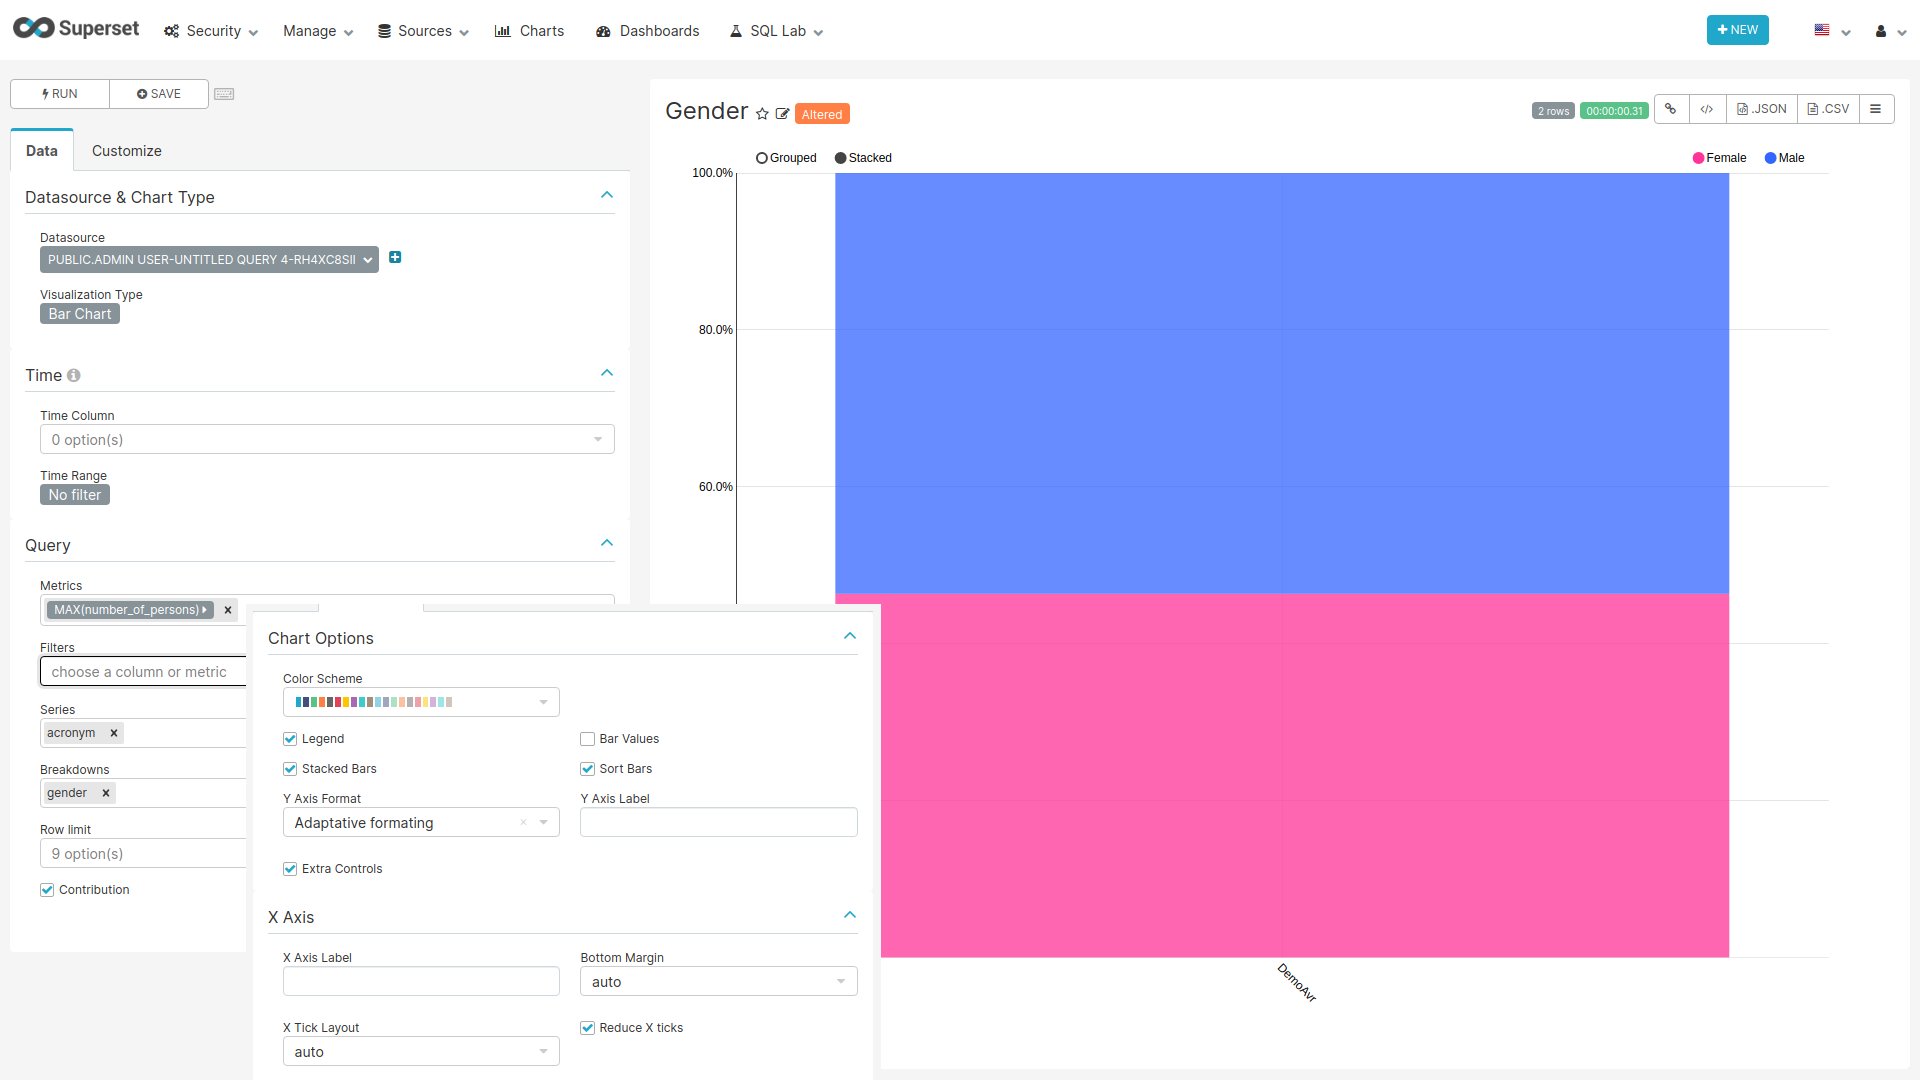
\includegraphics[width=1\linewidth]{images/04-person/05-gender} \caption{Settings for creating the Gender chart}\label{fig:gender}
\end{figure}

\hypertarget{sql-query-18}{%
\subsubsection*{SQL query}\label{sql-query-18}}
\addcontentsline{toc}{subsubsection}{SQL query}

\begin{Shaded}
\begin{Highlighting}[]
\KeywordTok{SELECT} \KeywordTok{source}\NormalTok{.name,}
\NormalTok{       concept\_name }\KeywordTok{AS}\NormalTok{ Gender, }
\NormalTok{       count\_value }\KeywordTok{AS}\NormalTok{ Number\_of\_persons,}
       \KeywordTok{source}\NormalTok{.acronym}
\KeywordTok{FROM} \KeywordTok{public}\NormalTok{.achilles\_results }\KeywordTok{AS}\NormalTok{ achilles}
\KeywordTok{INNER} \KeywordTok{JOIN} \KeywordTok{public}\NormalTok{.data\_source }\KeywordTok{AS} \KeywordTok{source} \KeywordTok{ON}\NormalTok{ achilles.data\_source\_id}\OperatorTok{=}\KeywordTok{source}\NormalTok{.}\KeywordTok{id}
\KeywordTok{JOIN}\NormalTok{ (}
  \KeywordTok{SELECT} \StringTok{\textquotesingle{}8507\textquotesingle{}} \KeywordTok{AS}\NormalTok{ concept\_id, }\StringTok{\textquotesingle{}Male\textquotesingle{}} \KeywordTok{AS}\NormalTok{ concept\_name}
  \KeywordTok{UNION}
  \KeywordTok{SELECT} \StringTok{\textquotesingle{}8532\textquotesingle{}} \KeywordTok{AS}\NormalTok{ concept\_id, }\StringTok{\textquotesingle{}Female\textquotesingle{}} \KeywordTok{AS}\NormalTok{ concept\_name}
\NormalTok{) }\KeywordTok{AS}\NormalTok{ concepts }\KeywordTok{ON}\NormalTok{ achilles.stratum\_1 }\OperatorTok{=}\NormalTok{ concept\_id}
\KeywordTok{WHERE}\NormalTok{ analysis\_id }\OperatorTok{=} \DecValTok{2}
\end{Highlighting}
\end{Shaded}

\hypertarget{chart-settings-20}{%
\subsubsection*{Chart settings}\label{chart-settings-20}}
\addcontentsline{toc}{subsubsection}{Chart settings}

\begin{itemize}
\tightlist
\item
  Data Tab

  \begin{itemize}
  \tightlist
  \item
    Datasource \& Chart Type

    \begin{itemize}
    \tightlist
    \item
      Visualization Type: Bar Chart
    \end{itemize}
  \item
    Time

    \begin{itemize}
    \tightlist
    \item
      Time range: No filter
    \end{itemize}
  \item
    Query

    \begin{itemize}
    \tightlist
    \item
      Metrics: MAX(Number\_of\_persons)
    \item
      Series: acronym
    \item
      Breakdowns: gender
    \item
      Contribution: on
    \end{itemize}
  \end{itemize}
\item
  Customize Tab

  \begin{itemize}
  \tightlist
  \item
    Chart Options

    \begin{itemize}
    \tightlist
    \item
      Stacked Bars: on
    \item
      Sort Bars: on
    \item
      Extra Controls: on
    \end{itemize}
  \item
    X Axis

    \begin{itemize}
    \tightlist
    \item
      Reduce X ticks: on
    \end{itemize}
  \end{itemize}
\end{itemize}

\hypertarget{observation-period-deprecated}{%
\section{Observation Period {[}Deprecated{]}}\label{observation-period-deprecated}}

\hypertarget{css-4}{%
\subsection*{CSS}\label{css-4}}
\addcontentsline{toc}{subsection}{CSS}

To hide the dashboard header insert the following css code to the \texttt{CSS} field on the edit page:

\begin{Shaded}
\begin{Highlighting}[]
\FunctionTok{.dashboard} \OperatorTok{\textgreater{}}\NormalTok{ div}\InformationTok{:not(}\FunctionTok{.dashboard{-}content}\InformationTok{)}\NormalTok{ \{  }\CommentTok{/* dashboard header */}
  \KeywordTok{display}\NormalTok{: }\DecValTok{none}\OperatorTok{;}
\NormalTok{\}}
\end{Highlighting}
\end{Shaded}

With this every time you want to edit the dashboard layout you have to either comment the CSS inserted
or remove it so the ``Edit Dashboard'' button can show again.

\hypertarget{data-source-filter-2}{%
\subsection*{Data Source Filter}\label{data-source-filter-2}}
\addcontentsline{toc}{subsection}{Data Source Filter}

\begin{figure}
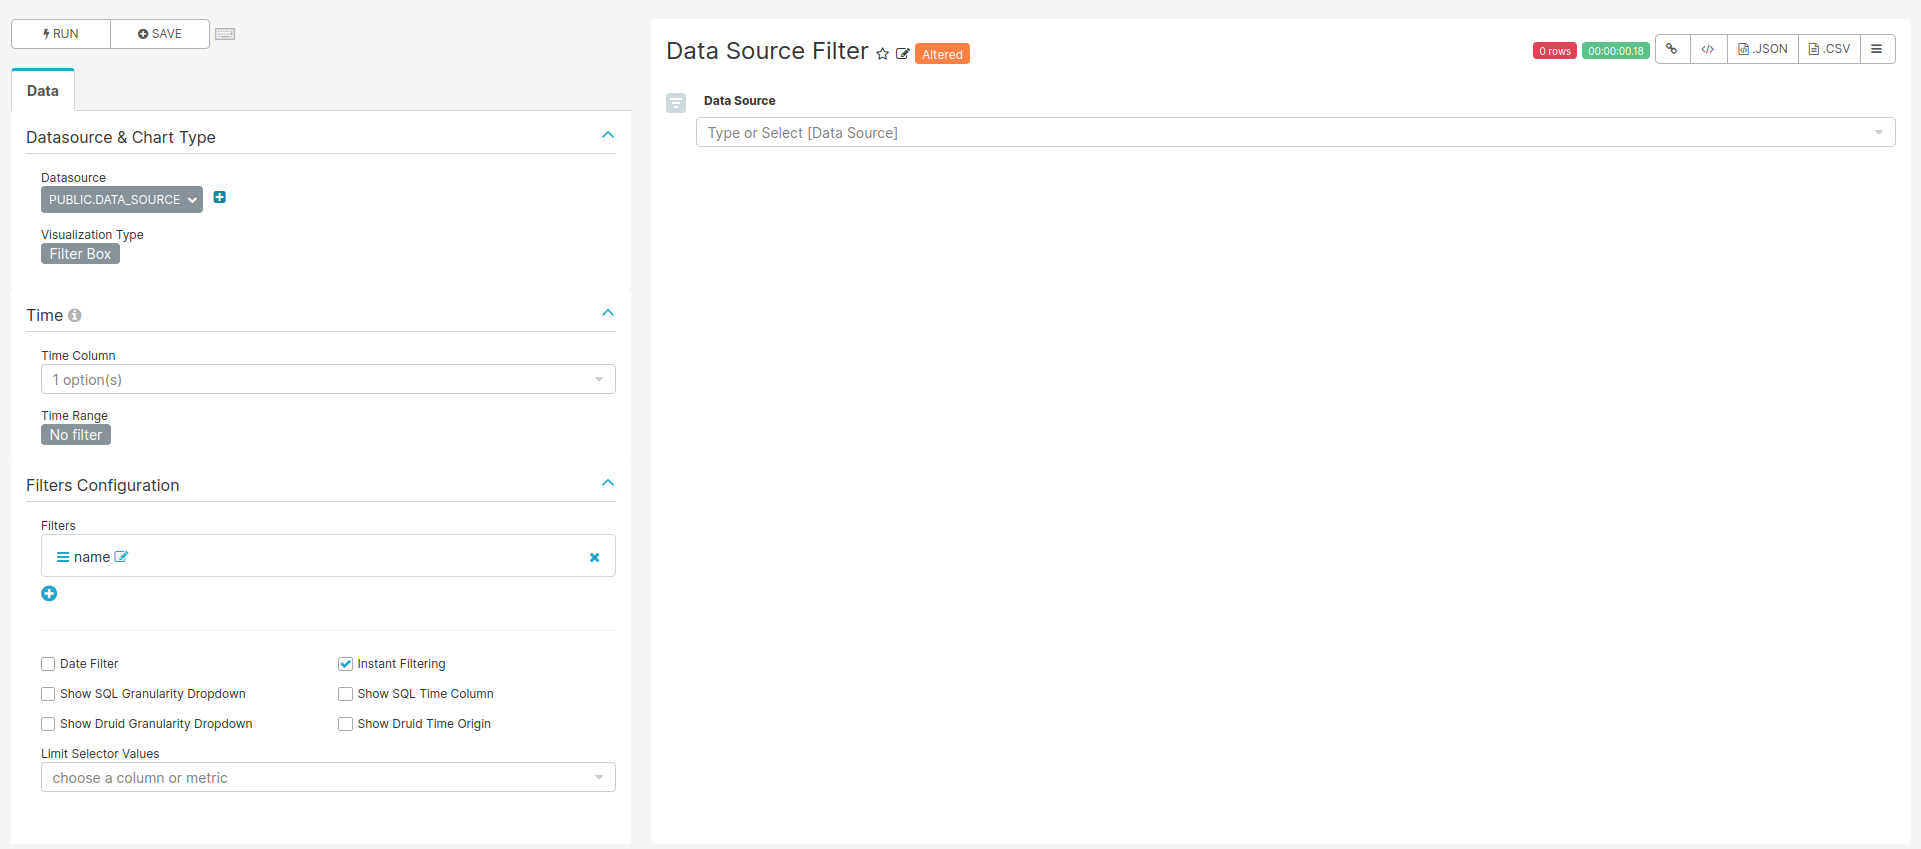
\includegraphics[width=1\linewidth]{images/shared/data_source_filter} \caption{Settings for creating the Data Source filter chart}\label{fig:dataSourceFilter}
\end{figure}

\textbf{For the filter to work the name of the fields to filter should match in all tables used on the charts of this dashboard.}

\hypertarget{sql-query-19}{%
\subsubsection*{SQL query}\label{sql-query-19}}
\addcontentsline{toc}{subsubsection}{SQL query}

No SQL query, use the sql table \texttt{data\_source} of the \texttt{achilles} database.

\hypertarget{chart-settings-21}{%
\subsubsection*{Chart settings}\label{chart-settings-21}}
\addcontentsline{toc}{subsubsection}{Chart settings}

\begin{itemize}
\tightlist
\item
  Data Tab

  \begin{itemize}
  \tightlist
  \item
    Datasource \& Chart Type

    \begin{itemize}
    \tightlist
    \item
      Visualization Type: Filter Box
    \end{itemize}
  \item
    Time

    \begin{itemize}
    \tightlist
    \item
      Time range: No filter
    \end{itemize}
  \item
    Filters Configuration

    \begin{itemize}
    \tightlist
    \item
      Filters:

      \begin{itemize}
      \tightlist
      \item
        name
      \end{itemize}
    \item
      Date Filter: off
    \item
      Instant Filtering: on
    \end{itemize}
  \end{itemize}
\end{itemize}

\hypertarget{number-of-patients-in-observation-period-numinobservationperiod}{%
\subsection*{Number of Patients in Observation Period \{\#numInObservationPeriod\}}\label{number-of-patients-in-observation-period-numinobservationperiod}}
\addcontentsline{toc}{subsection}{Number of Patients in Observation Period \{\#numInObservationPeriod\}}

The Number of Patients in Observation Period plot shows the number of patients that contribute at least one day in a specific month.

\begin{figure}
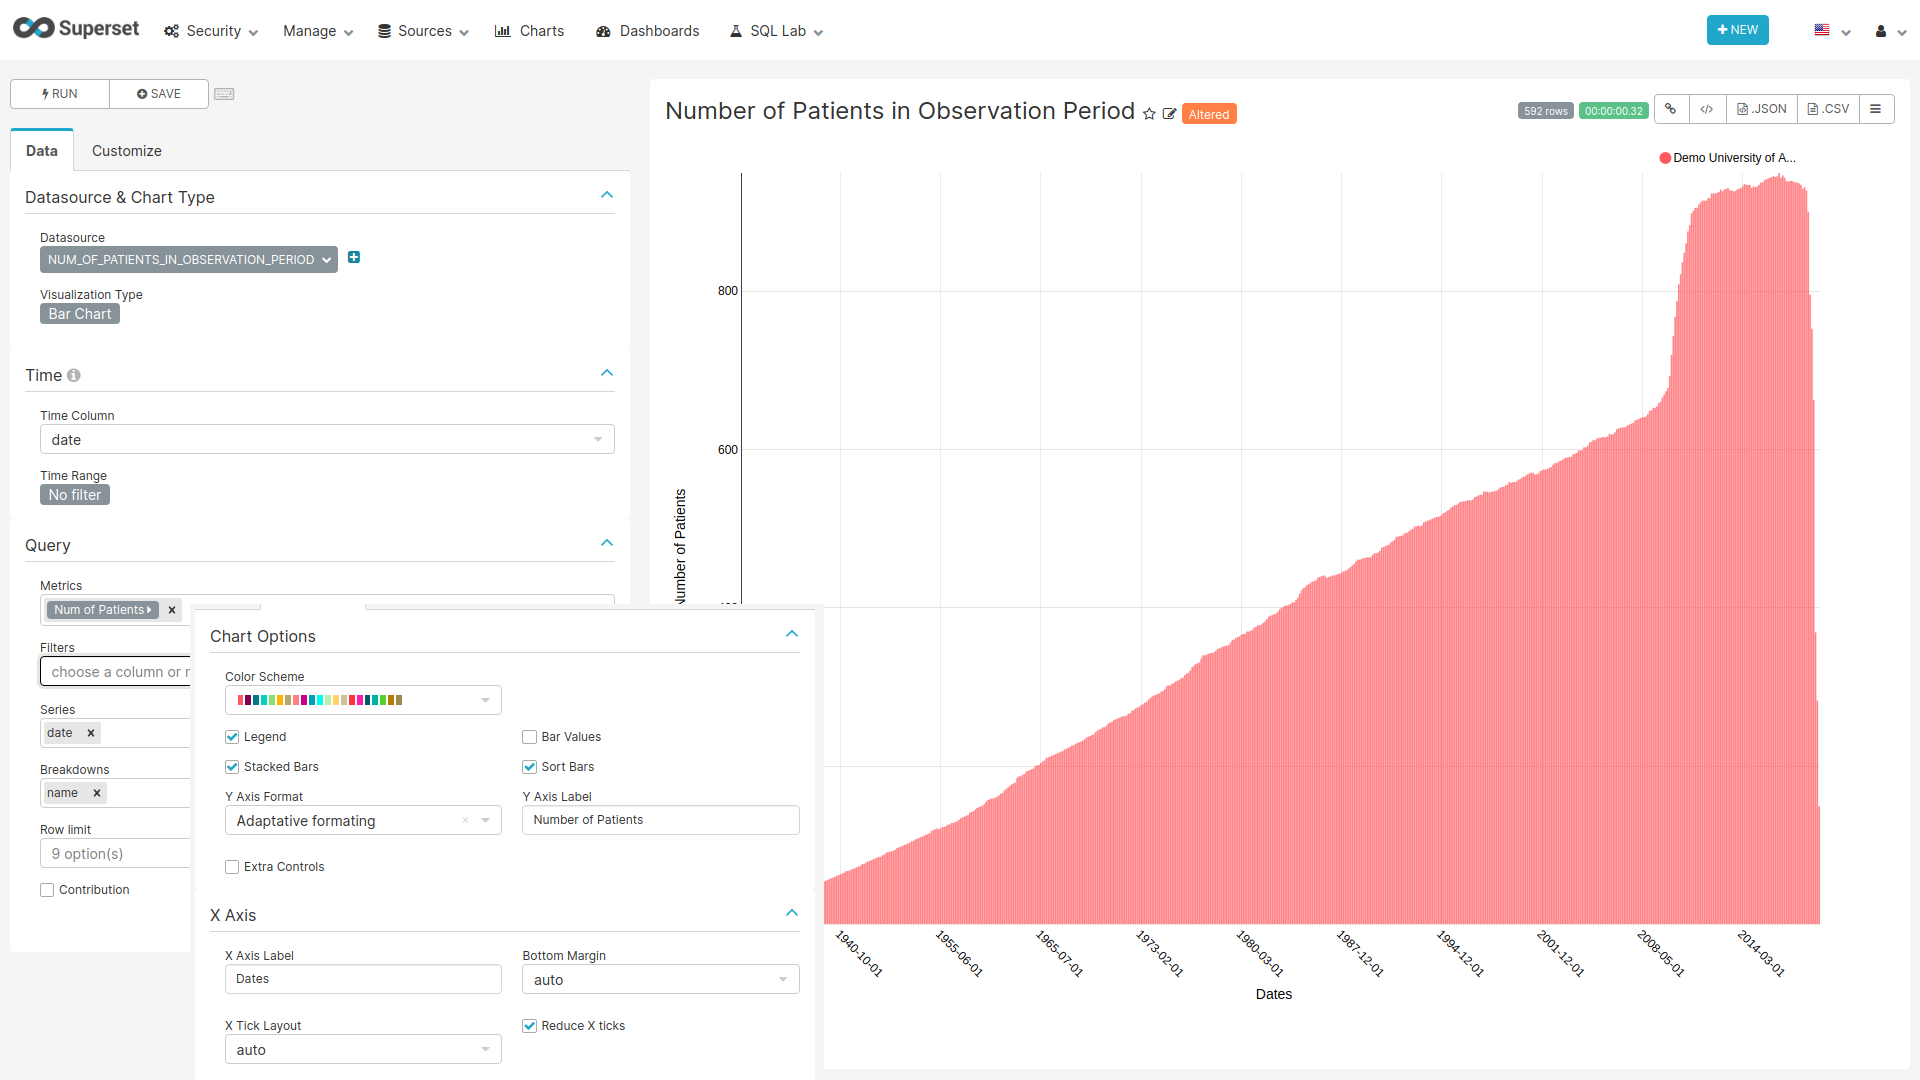
\includegraphics[width=1\linewidth]{images/05-observation_period/02-number_of_patients_in_observation_period} \caption{Settings for creating the Number of Patients in Observation Period chart}\label{fig:numPatientsInObserPeriod}
\end{figure}

\hypertarget{sql-query-20}{%
\subsubsection*{SQL query}\label{sql-query-20}}
\addcontentsline{toc}{subsubsection}{SQL query}

\begin{Shaded}
\begin{Highlighting}[]
\KeywordTok{SELECT} \KeywordTok{source}\NormalTok{.name,}
       \KeywordTok{source}\NormalTok{.acronym,}
       \FunctionTok{to\_date}\NormalTok{(stratum\_1, }\StringTok{\textquotesingle{}YYYYMM\textquotesingle{}}\NormalTok{) }\KeywordTok{as} \DataTypeTok{Date}\NormalTok{,}
\NormalTok{       count\_value}
\KeywordTok{FROM} \KeywordTok{public}\NormalTok{.achilles\_results }\KeywordTok{AS}\NormalTok{ achilles}
\KeywordTok{INNER} \KeywordTok{JOIN} \KeywordTok{public}\NormalTok{.data\_source }\KeywordTok{AS} \KeywordTok{source} \KeywordTok{ON}\NormalTok{ achilles.data\_source\_id}\OperatorTok{=}\KeywordTok{source}\NormalTok{.}\KeywordTok{id}
\KeywordTok{WHERE}\NormalTok{ analysis\_id }\OperatorTok{=} \DecValTok{110}
\end{Highlighting}
\end{Shaded}

\hypertarget{chart-settings-22}{%
\subsubsection*{Chart settings}\label{chart-settings-22}}
\addcontentsline{toc}{subsubsection}{Chart settings}

\begin{itemize}
\tightlist
\item
  Data Tab

  \begin{itemize}
  \tightlist
  \item
    Datasource \& Chart Type

    \begin{itemize}
    \tightlist
    \item
      Visualization Type: Bar Chart
    \end{itemize}
  \item
    Time

    \begin{itemize}
    \tightlist
    \item
      Time range: No filter
    \end{itemize}
  \item
    Query

    \begin{itemize}
    \tightlist
    \item
      Metrics: MAX(count\_value) with label ``Num of Patients''
    \item
      Series: date
    \item
      Breakdowns: name
    \end{itemize}
  \end{itemize}
\item
  Customize Tab

  \begin{itemize}
  \tightlist
  \item
    Chart Options

    \begin{itemize}
    \tightlist
    \item
      Stacked Bars: on
    \item
      Sort Bars: on
    \item
      Y Axis Label: Number of Patients
    \end{itemize}
  \item
    X Axis

    \begin{itemize}
    \tightlist
    \item
      X Axis Label: Dates
    \item
      Reduce X ticks: on
    \end{itemize}
  \end{itemize}
\end{itemize}

\hypertarget{observation-period-start-dates}{%
\subsection*{Observation Period Start Dates}\label{observation-period-start-dates}}
\addcontentsline{toc}{subsection}{Observation Period Start Dates}

\begin{figure}
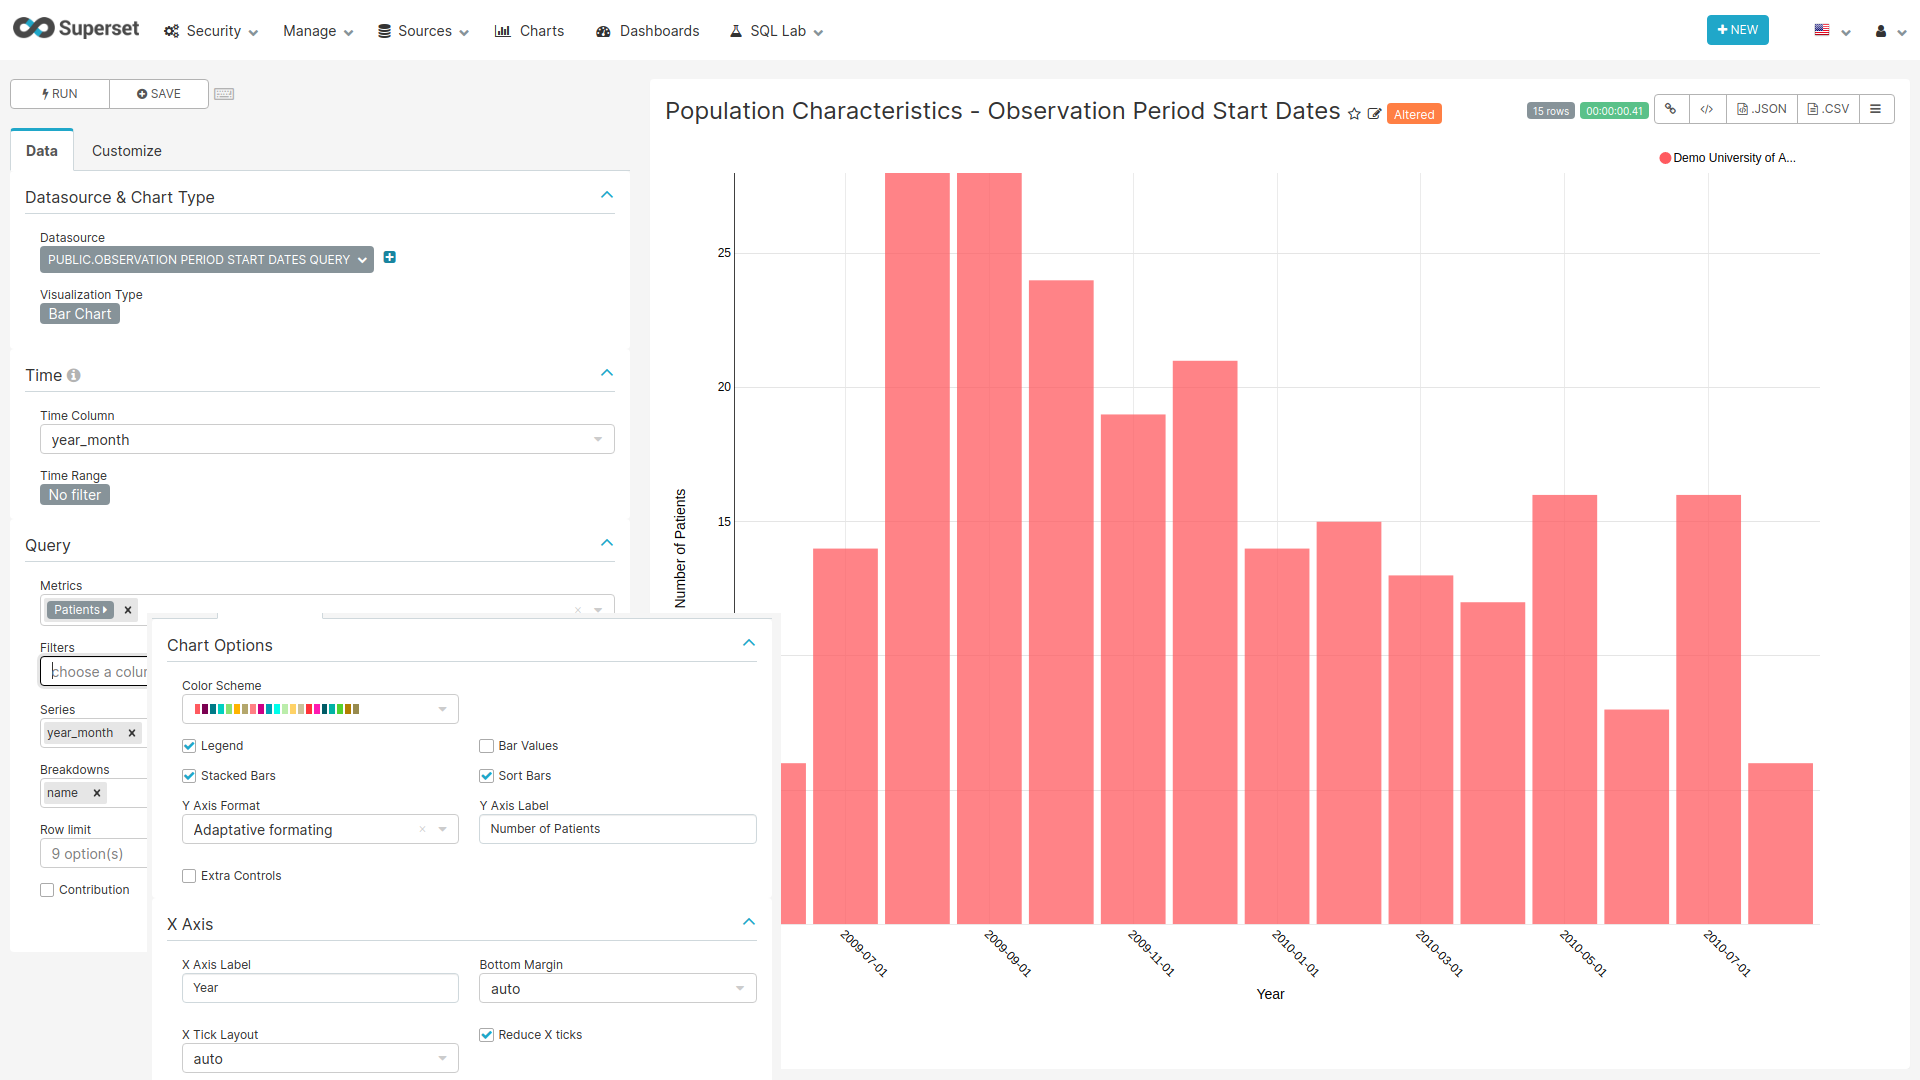
\includegraphics[width=1\linewidth]{images/05-observation_period/03-observation_period_start_dates} \caption{Settings for creating the Observation Period Start Dates chart}\label{fig:observationPeriodStartDates}
\end{figure}

\hypertarget{sql-query-21}{%
\subsubsection*{SQL query}\label{sql-query-21}}
\addcontentsline{toc}{subsubsection}{SQL query}

\begin{Shaded}
\begin{Highlighting}[]
\KeywordTok{SELECT} \KeywordTok{source}\NormalTok{.name,}
       \KeywordTok{source}\NormalTok{.acronym,}
       \FunctionTok{to\_date}\NormalTok{(stratum\_1, }\StringTok{\textquotesingle{}YYYYMM\textquotesingle{}}\NormalTok{) }\KeywordTok{AS}\NormalTok{ year\_month,}
\NormalTok{       count\_value}
\KeywordTok{FROM} \KeywordTok{public}\NormalTok{.achilles\_results }\KeywordTok{AS}\NormalTok{ achilles}
\KeywordTok{INNER} \KeywordTok{JOIN} \KeywordTok{public}\NormalTok{.data\_source }\KeywordTok{AS} \KeywordTok{source} \KeywordTok{ON}\NormalTok{ achilles.data\_source\_id}\OperatorTok{=}\KeywordTok{source}\NormalTok{.}\KeywordTok{id}
\KeywordTok{WHERE}\NormalTok{ analysis\_id }\OperatorTok{=} \DecValTok{111}
\end{Highlighting}
\end{Shaded}

\hypertarget{chart-settings-23}{%
\subsubsection*{Chart settings}\label{chart-settings-23}}
\addcontentsline{toc}{subsubsection}{Chart settings}

\begin{itemize}
\tightlist
\item
  Data Tab

  \begin{itemize}
  \tightlist
  \item
    Datasource \& Chart Type

    \begin{itemize}
    \tightlist
    \item
      Visualization Type: Bar Chart
    \end{itemize}
  \item
    Time

    \begin{itemize}
    \tightlist
    \item
      Time range: No filter
    \end{itemize}
  \item
    Query

    \begin{itemize}
    \tightlist
    \item
      Metrics: SUM(count\_value) with label ``Patients''
    \item
      Series: year\_month
    \item
      Breakdowns: name
    \end{itemize}
  \end{itemize}
\item
  Customize Tab

  \begin{itemize}
  \tightlist
  \item
    Chart Options

    \begin{itemize}
    \tightlist
    \item
      Stacked Bars: on
    \item
      Sort Bars: on
    \item
      Y Axis Label: Number of Patients
    \end{itemize}
  \item
    X Axis

    \begin{itemize}
    \tightlist
    \item
      X Axis Label: Year
    \item
      Reduce X ticks: on
    \end{itemize}
  \end{itemize}
\end{itemize}

\hypertarget{observation-period-end-dates}{%
\subsection*{Observation Period End Dates}\label{observation-period-end-dates}}
\addcontentsline{toc}{subsection}{Observation Period End Dates}

\begin{figure}
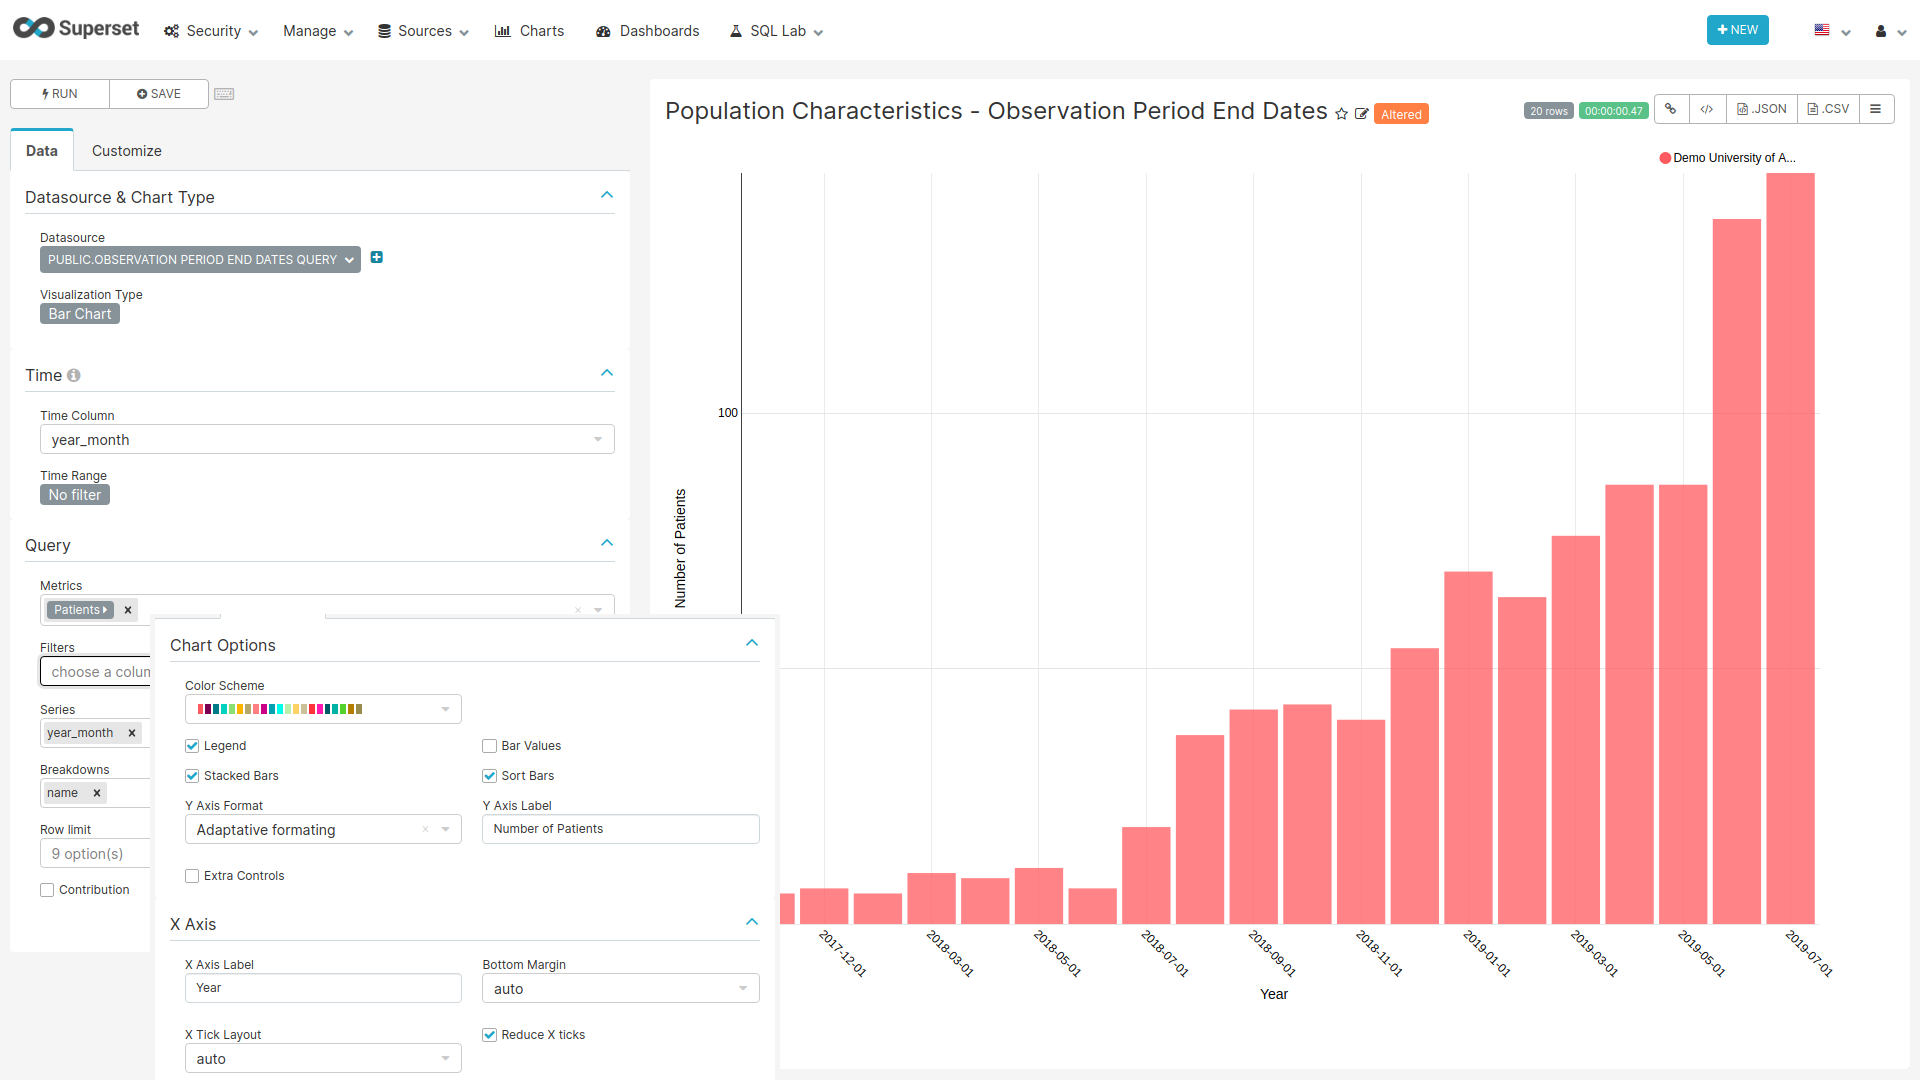
\includegraphics[width=1\linewidth]{images/05-observation_period/04-observation_period_end_dates} \caption{Settings for creating the Observation Period End Dates chart}\label{fig:observationPeriodEndDates}
\end{figure}

\hypertarget{sql-query-22}{%
\subsubsection*{SQL query}\label{sql-query-22}}
\addcontentsline{toc}{subsubsection}{SQL query}

\begin{Shaded}
\begin{Highlighting}[]
\KeywordTok{SELECT} \KeywordTok{source}\NormalTok{.name,}
       \KeywordTok{source}\NormalTok{.acronym,}
       \FunctionTok{to\_date}\NormalTok{(stratum\_1, }\StringTok{\textquotesingle{}YYYYMM\textquotesingle{}}\NormalTok{) }\KeywordTok{AS}\NormalTok{ year\_month,}
\NormalTok{       count\_value}
\KeywordTok{FROM} \KeywordTok{public}\NormalTok{.achilles\_results }\KeywordTok{AS}\NormalTok{ achilles}
\KeywordTok{INNER} \KeywordTok{JOIN} \KeywordTok{public}\NormalTok{.data\_source }\KeywordTok{AS} \KeywordTok{source} \KeywordTok{ON}\NormalTok{ achilles.data\_source\_id}\OperatorTok{=}\KeywordTok{source}\NormalTok{.}\KeywordTok{id}
\KeywordTok{WHERE}\NormalTok{ analysis\_id }\OperatorTok{=} \DecValTok{112}
\end{Highlighting}
\end{Shaded}

\hypertarget{chart-settings-24}{%
\subsubsection*{Chart settings}\label{chart-settings-24}}
\addcontentsline{toc}{subsubsection}{Chart settings}

\begin{itemize}
\tightlist
\item
  Data Tab

  \begin{itemize}
  \tightlist
  \item
    Datasource \& Chart Type

    \begin{itemize}
    \tightlist
    \item
      Visualization Type: Bar Chart
    \end{itemize}
  \item
    Time

    \begin{itemize}
    \tightlist
    \item
      Time range: No filter
    \end{itemize}
  \item
    Query

    \begin{itemize}
    \tightlist
    \item
      Metrics: SUM(count\_value) with label ``Patients''
    \item
      Series: year\_month
    \item
      Breakdowns: name
    \end{itemize}
  \end{itemize}
\item
  Customize Tab

  \begin{itemize}
  \tightlist
  \item
    Chart Options

    \begin{itemize}
    \tightlist
    \item
      Stacked Bars: on
    \item
      Sort Bars: on
    \item
      Y Axis Label: Number of Patients
    \end{itemize}
  \item
    X Axis

    \begin{itemize}
    \tightlist
    \item
      X Axis Label: Year
    \item
      Reduce X ticks: on
    \end{itemize}
  \end{itemize}
\end{itemize}

\hypertarget{visit-deprecated}{%
\section{Visit {[}Deprecated{]}}\label{visit-deprecated}}

This dashboard shows the different types of visits per data source (see \href{https://ohdsi.github.io/CommonDataModel/cdm531.html\#visit_occurrence}{Visit Occurence Table})

\hypertarget{css-5}{%
\subsection*{CSS}\label{css-5}}
\addcontentsline{toc}{subsection}{CSS}

To hide the dashboard header insert the following css code to the \texttt{CSS} field on the edit page:

\begin{Shaded}
\begin{Highlighting}[]
\FunctionTok{.dashboard} \OperatorTok{\textgreater{}}\NormalTok{ div}\InformationTok{:not(}\FunctionTok{.dashboard{-}content}\InformationTok{)}\NormalTok{ \{  }\CommentTok{/* dashboard header */}
  \KeywordTok{display}\NormalTok{: }\DecValTok{none}\OperatorTok{;}
\NormalTok{\}}
\end{Highlighting}
\end{Shaded}

With this every time you want to edit the dashboard layout you have to either comment the CSS inserted
or remove it so the ``Edit Dashboard'' button can show again.

\hypertarget{data-source-filter-3}{%
\subsection*{Data Source Filter}\label{data-source-filter-3}}
\addcontentsline{toc}{subsection}{Data Source Filter}

\begin{figure}
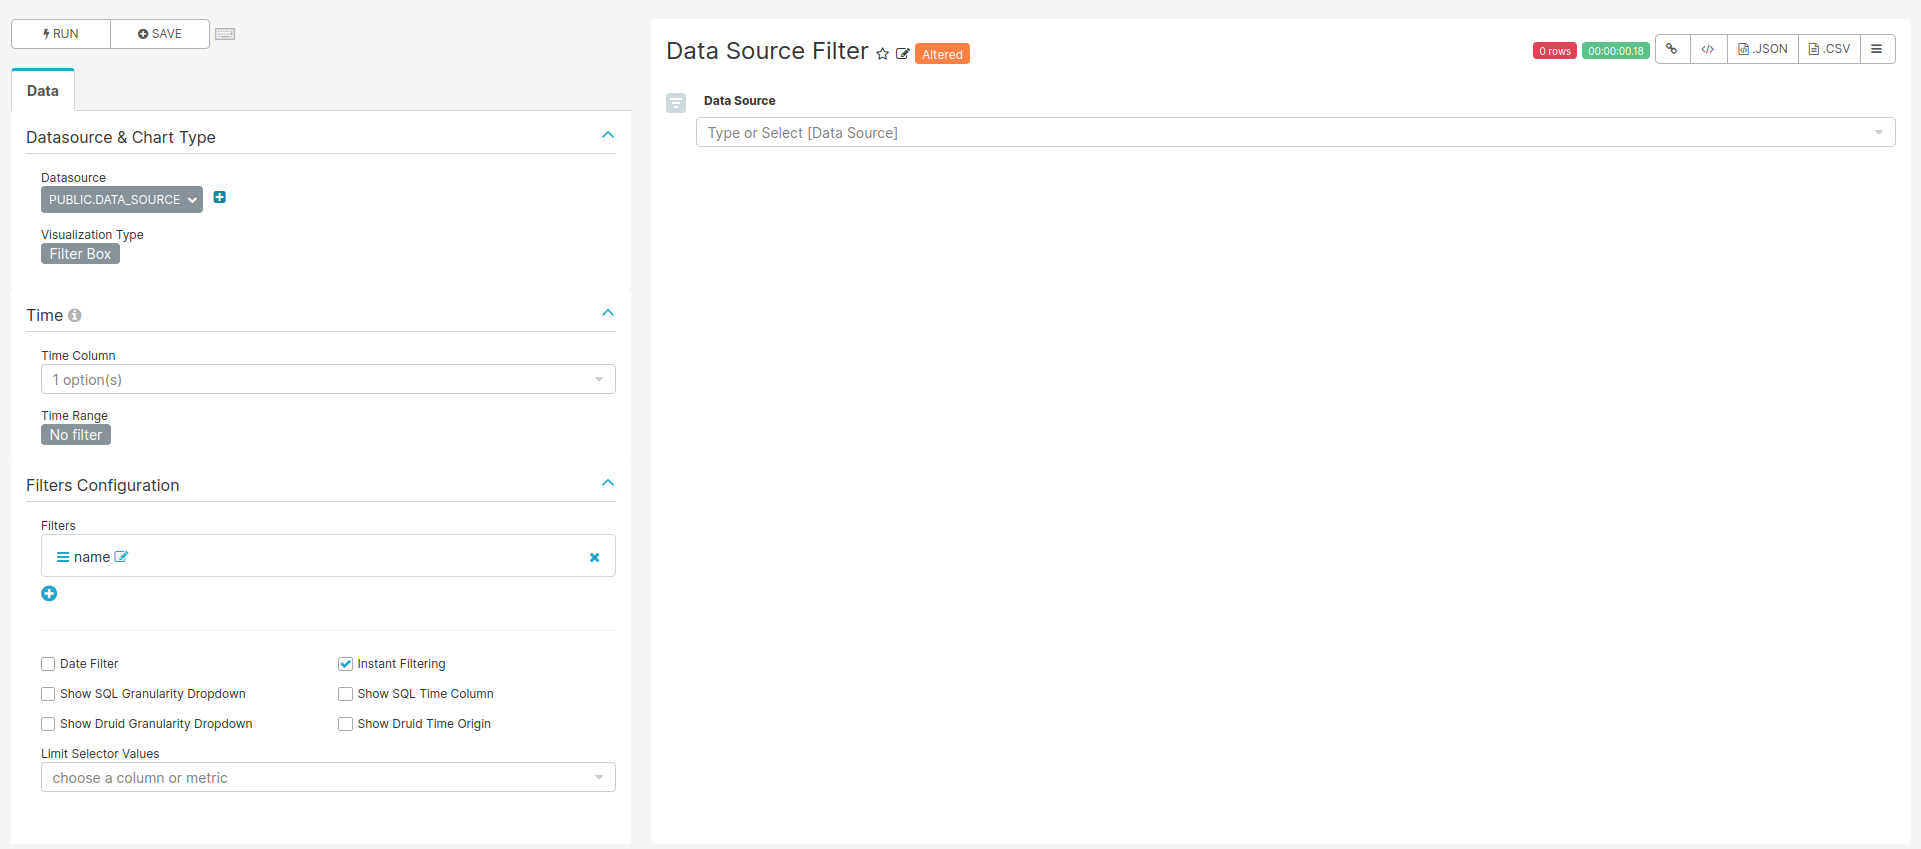
\includegraphics[width=1\linewidth]{images/shared/data_source_filter} \caption{Settings for creating the Data Source filter chart}\label{fig:dataSourceFilter}
\end{figure}

\textbf{For the filter to work the name of the fields to filter should match in all tables used on the charts of this dashboard.}

\hypertarget{sql-query-23}{%
\subsubsection*{SQL query}\label{sql-query-23}}
\addcontentsline{toc}{subsubsection}{SQL query}

No SQL query, use the sql table \texttt{data\_source} of the \texttt{achilles} database.

\hypertarget{chart-settings-25}{%
\subsubsection*{Chart settings}\label{chart-settings-25}}
\addcontentsline{toc}{subsubsection}{Chart settings}

\begin{itemize}
\tightlist
\item
  Data Tab

  \begin{itemize}
  \tightlist
  \item
    Datasource \& Chart Type

    \begin{itemize}
    \tightlist
    \item
      Visualization Type: Filter Box
    \end{itemize}
  \item
    Time

    \begin{itemize}
    \tightlist
    \item
      Time range: No filter
    \end{itemize}
  \item
    Filters Configuration

    \begin{itemize}
    \tightlist
    \item
      Filters:

      \begin{itemize}
      \tightlist
      \item
        name
      \end{itemize}
    \item
      Date Filter: off
    \item
      Instant Filtering: on
    \end{itemize}
  \end{itemize}
\end{itemize}

\hypertarget{visit-type-table-visittypetable}{%
\subsection*{Visit Type Table \{\#visitTypeTable\}}\label{visit-type-table-visittypetable}}
\addcontentsline{toc}{subsection}{Visit Type Table \{\#visitTypeTable\}}

\begin{figure}
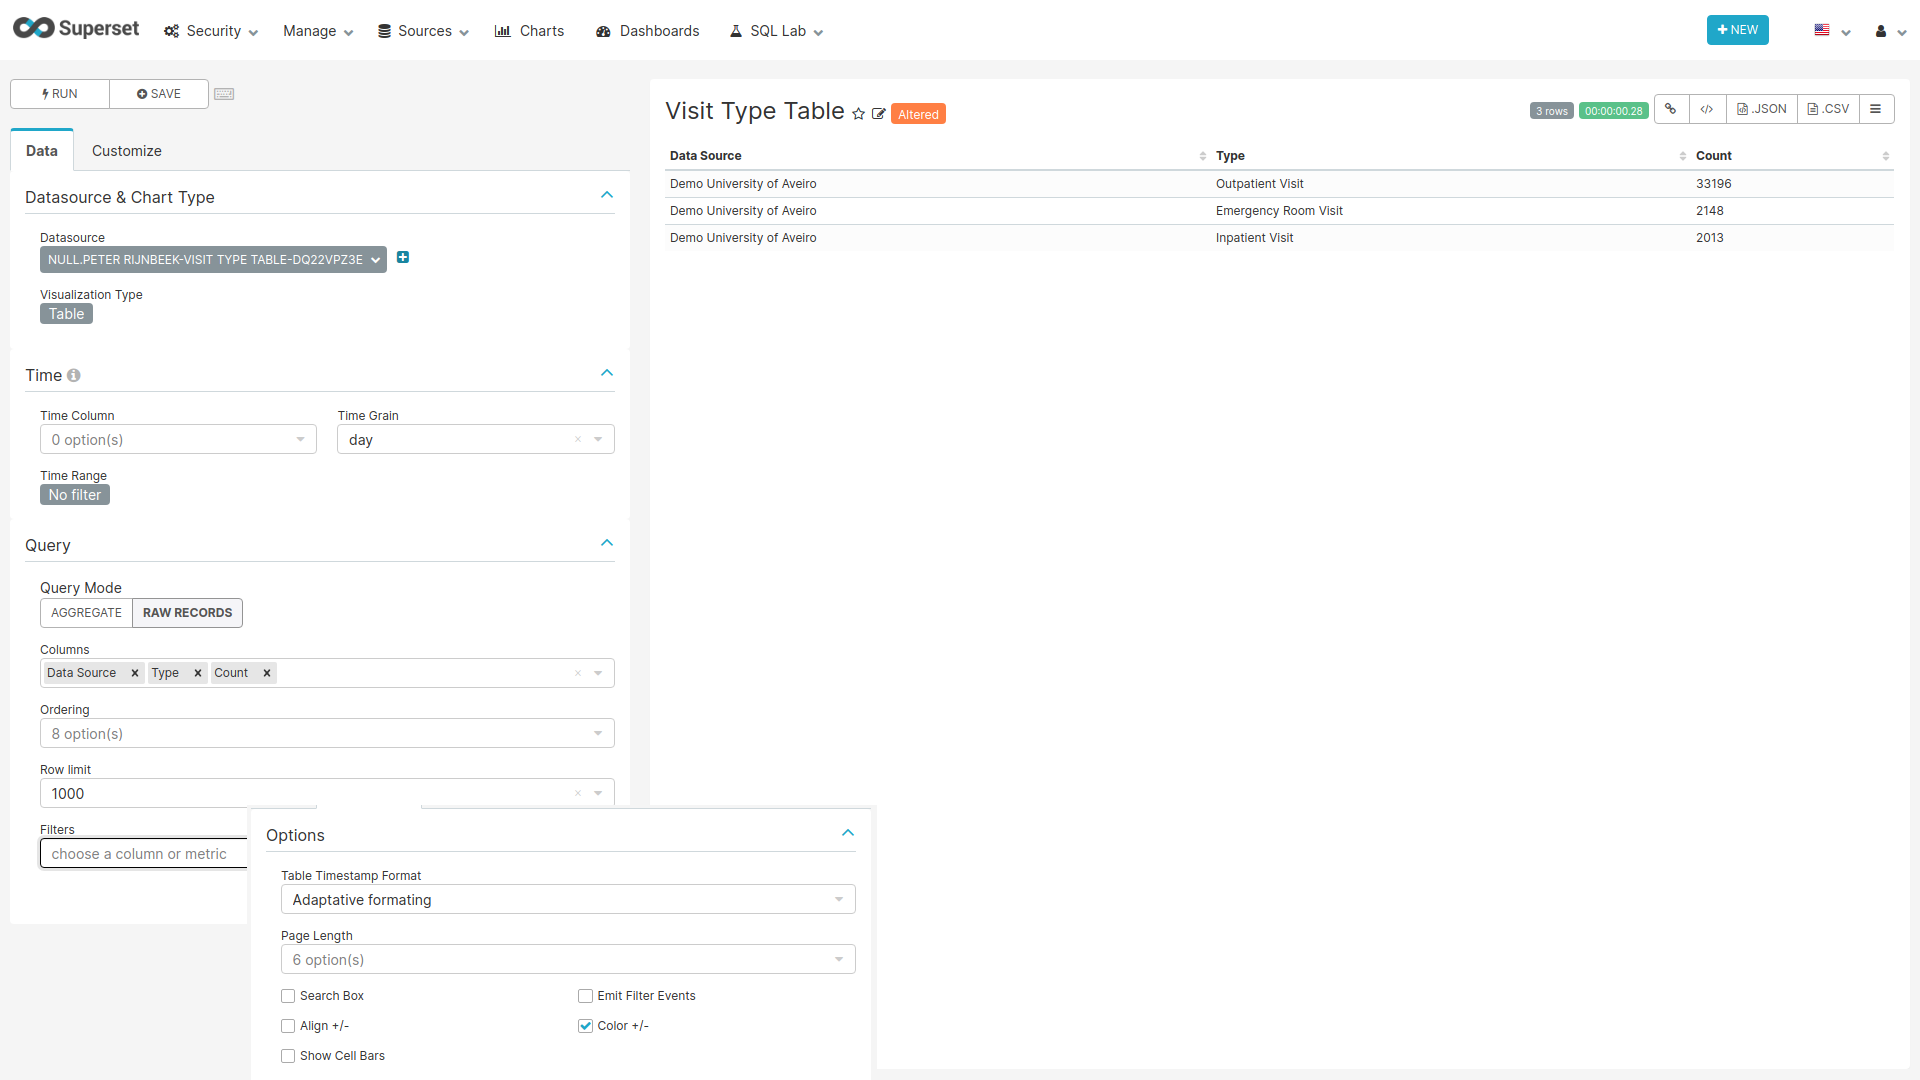
\includegraphics[width=1\linewidth]{images/06-visit/02-visit_types_table} \caption{Settings for creating the Visit Type Table chart}\label{fig:visitTypeTable}
\end{figure}

\hypertarget{sql-query-24}{%
\subsubsection*{SQL query}\label{sql-query-24}}
\addcontentsline{toc}{subsubsection}{SQL query}

\begin{Shaded}
\begin{Highlighting}[]
\KeywordTok{SELECT} \KeywordTok{source}\NormalTok{.name,}
       \KeywordTok{source}\NormalTok{.acronym,}
\NormalTok{       concept\_name }\KeywordTok{AS} \OtherTok{"Type"}\NormalTok{,}
       \FunctionTok{MAX}\NormalTok{(count\_value) }\KeywordTok{AS} \OtherTok{"Count"}
\KeywordTok{FROM} \KeywordTok{public}\NormalTok{.achilles\_results }\KeywordTok{AS}\NormalTok{ achilles}
\KeywordTok{INNER} \KeywordTok{JOIN} \KeywordTok{public}\NormalTok{.data\_source }\KeywordTok{AS} \KeywordTok{source} \KeywordTok{ON}\NormalTok{ achilles.data\_source\_id}\OperatorTok{=}\KeywordTok{source}\NormalTok{.}\KeywordTok{id}
\KeywordTok{INNER} \KeywordTok{JOIN} \KeywordTok{public}\NormalTok{.concept }\KeywordTok{ON} \FunctionTok{CAST}\NormalTok{(stratum\_1 }\KeywordTok{AS}\NormalTok{ BIGINT) }\OperatorTok{=}\NormalTok{ concept\_id}
\KeywordTok{WHERE}\NormalTok{ analysis\_id }\OperatorTok{=} \DecValTok{201}
\KeywordTok{GROUP} \KeywordTok{BY}\NormalTok{ name, acronym, }\OtherTok{"Type"}
\KeywordTok{ORDER} \KeywordTok{BY} \OtherTok{"Count"} \KeywordTok{DESC}
\end{Highlighting}
\end{Shaded}

\hypertarget{chart-settings-26}{%
\subsubsection*{Chart settings}\label{chart-settings-26}}
\addcontentsline{toc}{subsubsection}{Chart settings}

\begin{itemize}
\tightlist
\item
  Data Tab

  \begin{itemize}
  \tightlist
  \item
    Datasource \& Chart Type

    \begin{itemize}
    \tightlist
    \item
      Visualization Type: Table
    \end{itemize}
  \item
    Time

    \begin{itemize}
    \tightlist
    \item
      Time range: No filter
    \end{itemize}
  \item
    Query

    \begin{itemize}
    \tightlist
    \item
      Query Mode: Raw Records
    \item
      Columns: name with label ``Data Source'', Type, Count
    \end{itemize}
  \end{itemize}
\end{itemize}

\hypertarget{visit-types-bars}{%
\subsection*{Visit Types Bars}\label{visit-types-bars}}
\addcontentsline{toc}{subsection}{Visit Types Bars}

\begin{figure}
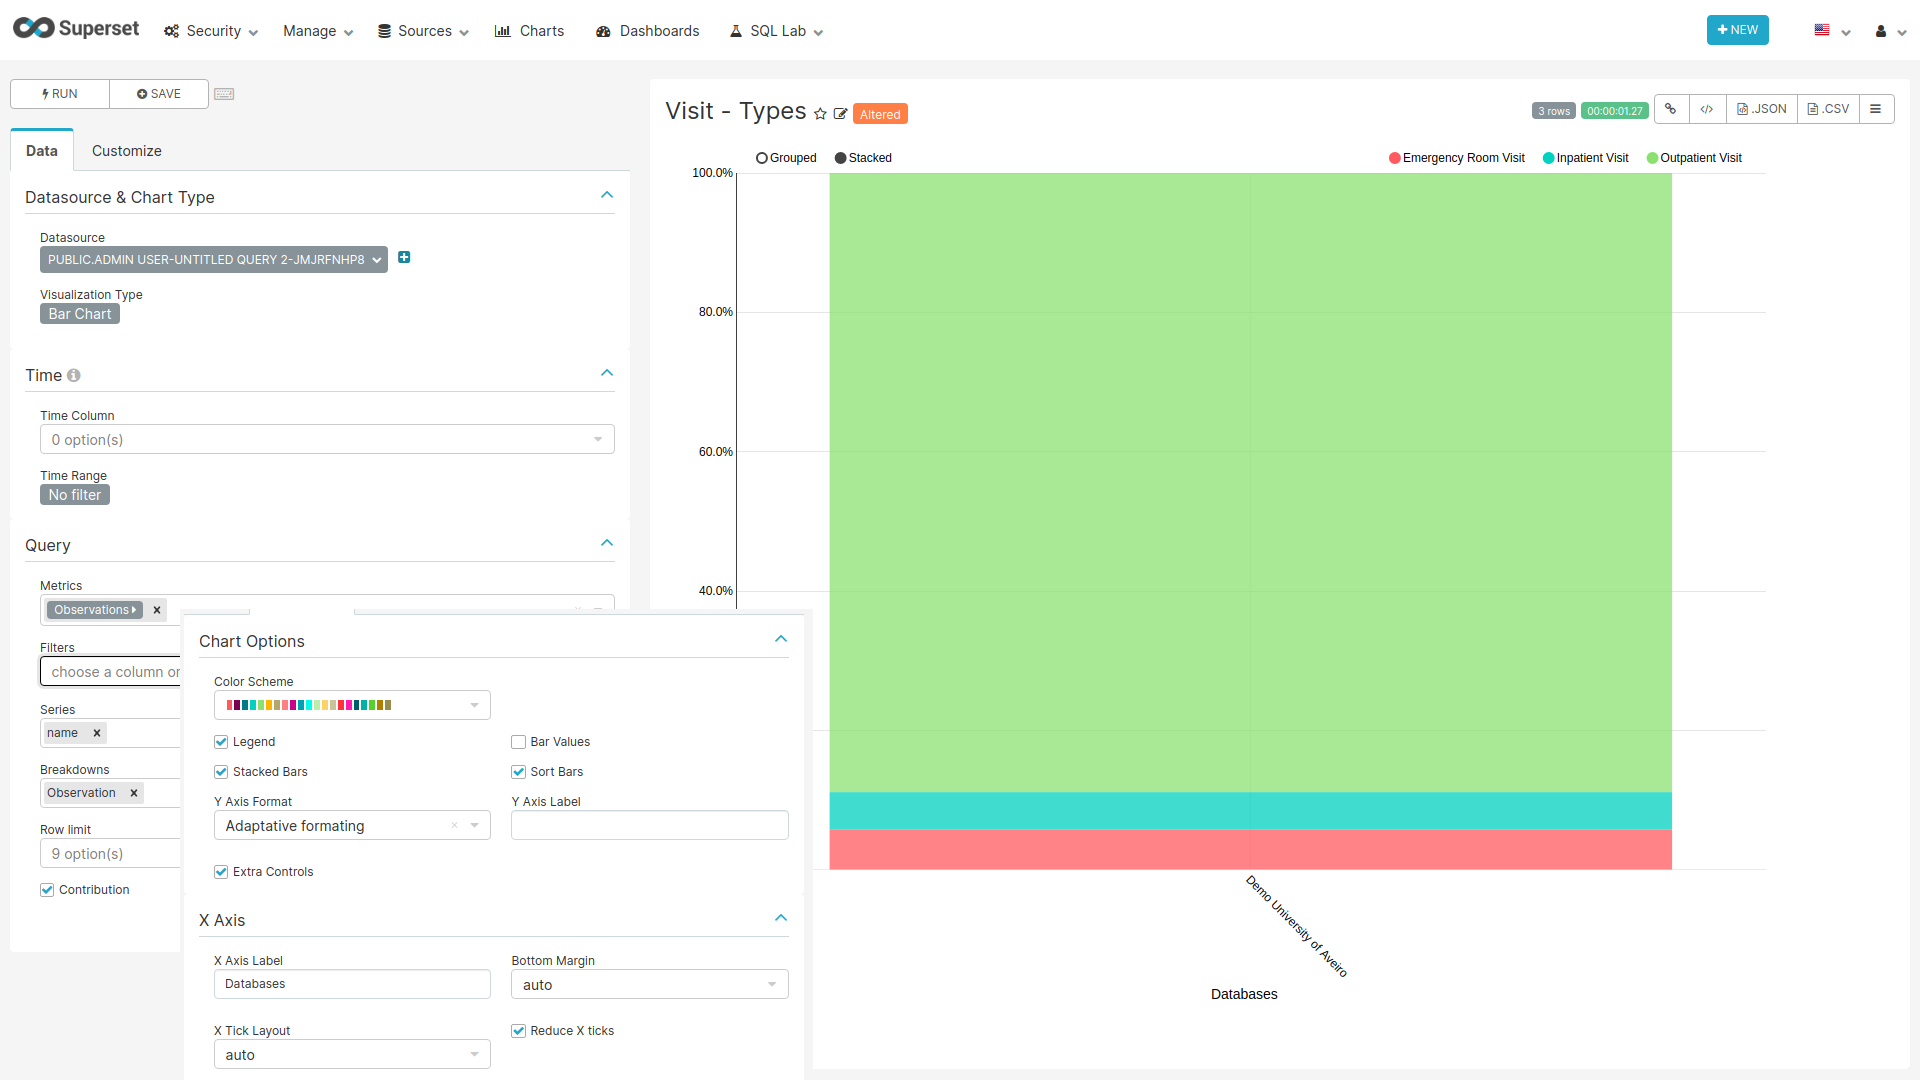
\includegraphics[width=1\linewidth]{images/06-visit/03-visit_types_bars} \caption{Settings for creating the Visit Types bar chart}\label{fig:visitTypeBars}
\end{figure}

\hypertarget{sql-query-25}{%
\subsubsection*{SQL query}\label{sql-query-25}}
\addcontentsline{toc}{subsubsection}{SQL query}

\begin{Shaded}
\begin{Highlighting}[]
\KeywordTok{SELECT} \KeywordTok{source}\NormalTok{.name, }
       \KeywordTok{source}\NormalTok{.acronym,}
\NormalTok{       concept\_name }\KeywordTok{AS} \OtherTok{"Observation"}\NormalTok{, }
\NormalTok{       count\_value}
\KeywordTok{FROM} \KeywordTok{public}\NormalTok{.achilles\_results }\KeywordTok{AS}\NormalTok{ achilles }
\KeywordTok{INNER} \KeywordTok{JOIN} \KeywordTok{public}\NormalTok{.data\_source }\KeywordTok{AS} \KeywordTok{source} \KeywordTok{ON}\NormalTok{ achilles.data\_source\_id}\OperatorTok{=}\KeywordTok{source}\NormalTok{.}\KeywordTok{id}
\KeywordTok{INNER} \KeywordTok{JOIN} \KeywordTok{public}\NormalTok{.concept }\KeywordTok{ON} \FunctionTok{CAST}\NormalTok{(stratum\_1 }\KeywordTok{AS}\NormalTok{ BIGINT) }\OperatorTok{=}\NormalTok{ concept\_id}
\KeywordTok{WHERE}\NormalTok{ analysis\_id }\OperatorTok{=} \DecValTok{201}
\end{Highlighting}
\end{Shaded}

\hypertarget{chart-settings-27}{%
\subsubsection*{Chart settings}\label{chart-settings-27}}
\addcontentsline{toc}{subsubsection}{Chart settings}

\begin{itemize}
\tightlist
\item
  Data Tab

  \begin{itemize}
  \tightlist
  \item
    Datasource \& Chart Type

    \begin{itemize}
    \tightlist
    \item
      Visualization Type: Bar Chart
    \end{itemize}
  \item
    Time

    \begin{itemize}
    \tightlist
    \item
      Time range: No filter
    \end{itemize}
  \item
    Query

    \begin{itemize}
    \tightlist
    \item
      Metrics: MAX(count\_value) with label Observations
    \item
      Series: name
    \item
      Breakdowns: Observation
    \end{itemize}
  \end{itemize}
\item
  Customize Tab

  \begin{itemize}
  \tightlist
  \item
    Chart Options

    \begin{itemize}
    \tightlist
    \item
      Stacked Bars: on
    \item
      Sort Bars: on
    \item
      Extra Controls: on
    \end{itemize}
  \item
    X Axis

    \begin{itemize}
    \tightlist
    \item
      X Axis Label: Databases
    \item
      Reduce X ticks: on
    \end{itemize}
  \end{itemize}
\end{itemize}

\hypertarget{death-deprecated}{%
\section{Death {[}Deprecated{]}}\label{death-deprecated}}

\hypertarget{css-6}{%
\subsection*{CSS}\label{css-6}}
\addcontentsline{toc}{subsection}{CSS}

To hide the dashboard header insert the following css code to the \texttt{CSS} field on the edit page:

\begin{Shaded}
\begin{Highlighting}[]
\FunctionTok{.dashboard} \OperatorTok{\textgreater{}}\NormalTok{ div}\InformationTok{:not(}\FunctionTok{.dashboard{-}content}\InformationTok{)}\NormalTok{ \{  }\CommentTok{/* dashboard header */}
  \KeywordTok{display}\NormalTok{: }\DecValTok{none}\OperatorTok{;}
\NormalTok{\}}
\end{Highlighting}
\end{Shaded}

With this every time you want to edit the dashboard layout you have to either comment the CSS inserted
or remove it so the ``Edit Dashboard'' button can show again.

\hypertarget{data-source-filter-4}{%
\subsection*{Data Source Filter}\label{data-source-filter-4}}
\addcontentsline{toc}{subsection}{Data Source Filter}

\begin{figure}
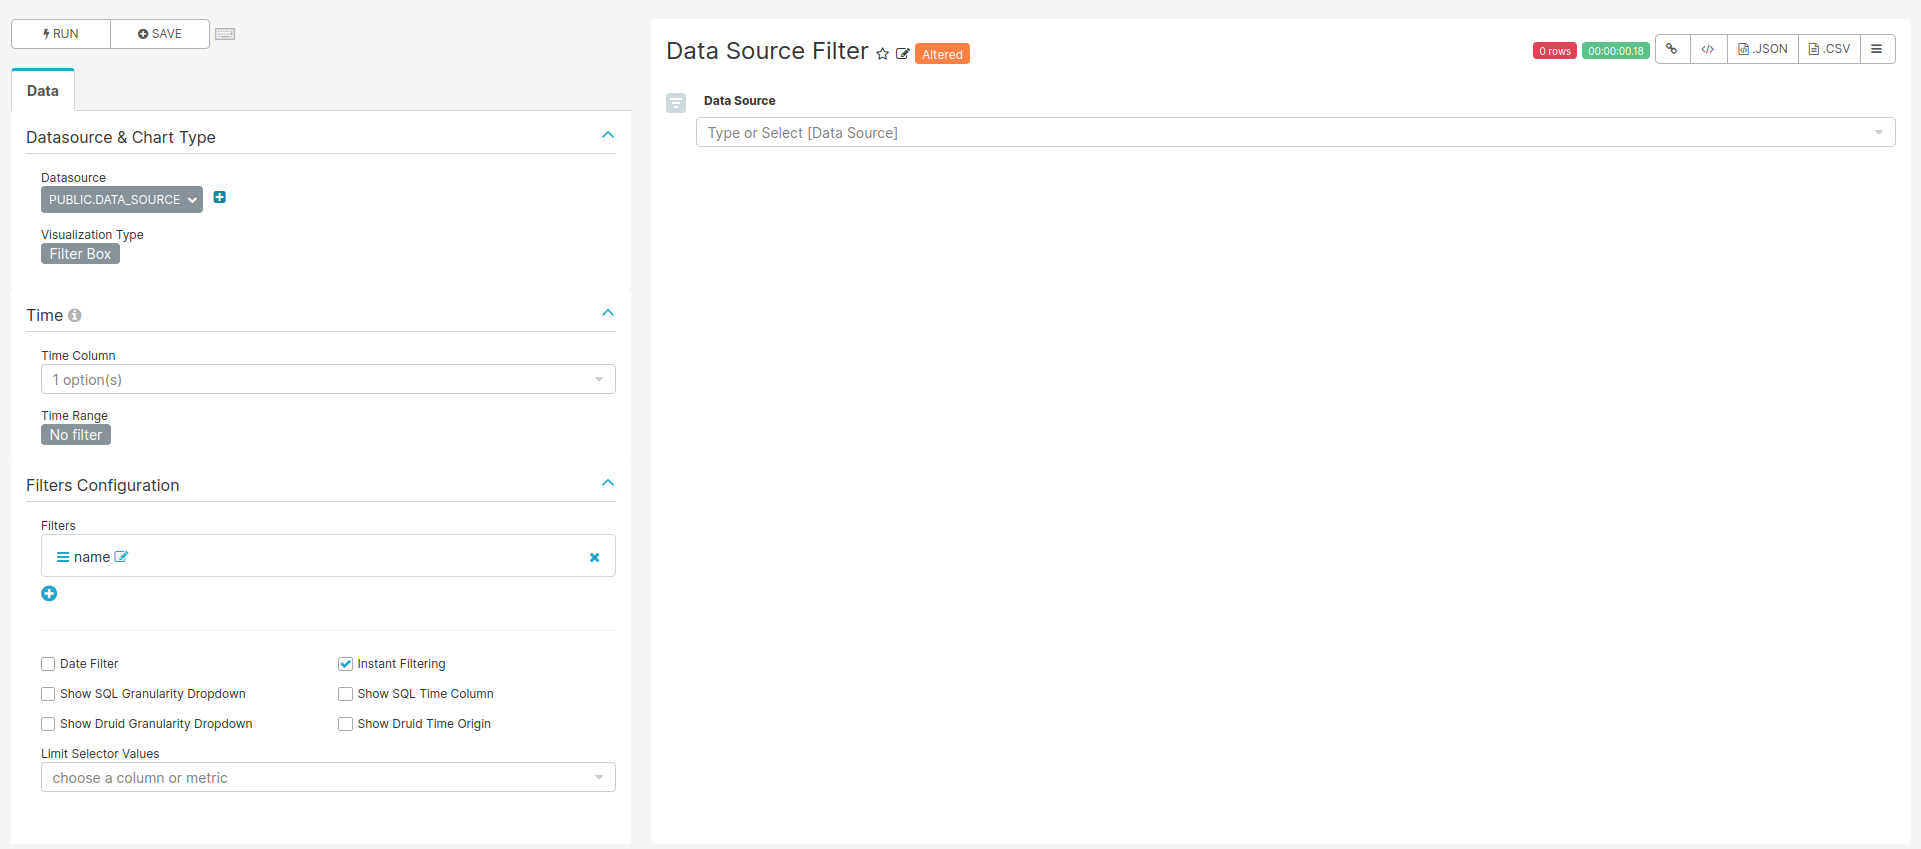
\includegraphics[width=1\linewidth]{images/shared/data_source_filter} \caption{Settings for creating the Data Source filter chart}\label{fig:dataSourceFilter}
\end{figure}

\textbf{For the filter to work the name of the fields to filter should match in all tables used on the charts of this dashboard.}

\hypertarget{sql-query-26}{%
\subsubsection*{SQL query}\label{sql-query-26}}
\addcontentsline{toc}{subsubsection}{SQL query}

No SQL query, use the sql table \texttt{data\_source} of the \texttt{achilles} database.

\hypertarget{chart-settings-28}{%
\subsubsection*{Chart settings}\label{chart-settings-28}}
\addcontentsline{toc}{subsubsection}{Chart settings}

\begin{itemize}
\tightlist
\item
  Data Tab

  \begin{itemize}
  \tightlist
  \item
    Datasource \& Chart Type

    \begin{itemize}
    \tightlist
    \item
      Visualization Type: Filter Box
    \end{itemize}
  \item
    Time

    \begin{itemize}
    \tightlist
    \item
      Time range: No filter
    \end{itemize}
  \item
    Filters Configuration

    \begin{itemize}
    \tightlist
    \item
      Filters:

      \begin{itemize}
      \tightlist
      \item
        name
      \end{itemize}
    \item
      Date Filter: off
    \item
      Instant Filtering: on
    \end{itemize}
  \end{itemize}
\end{itemize}

\hypertarget{number-of-records}{%
\subsection*{Number of Records}\label{number-of-records}}
\addcontentsline{toc}{subsection}{Number of Records}

\begin{figure}
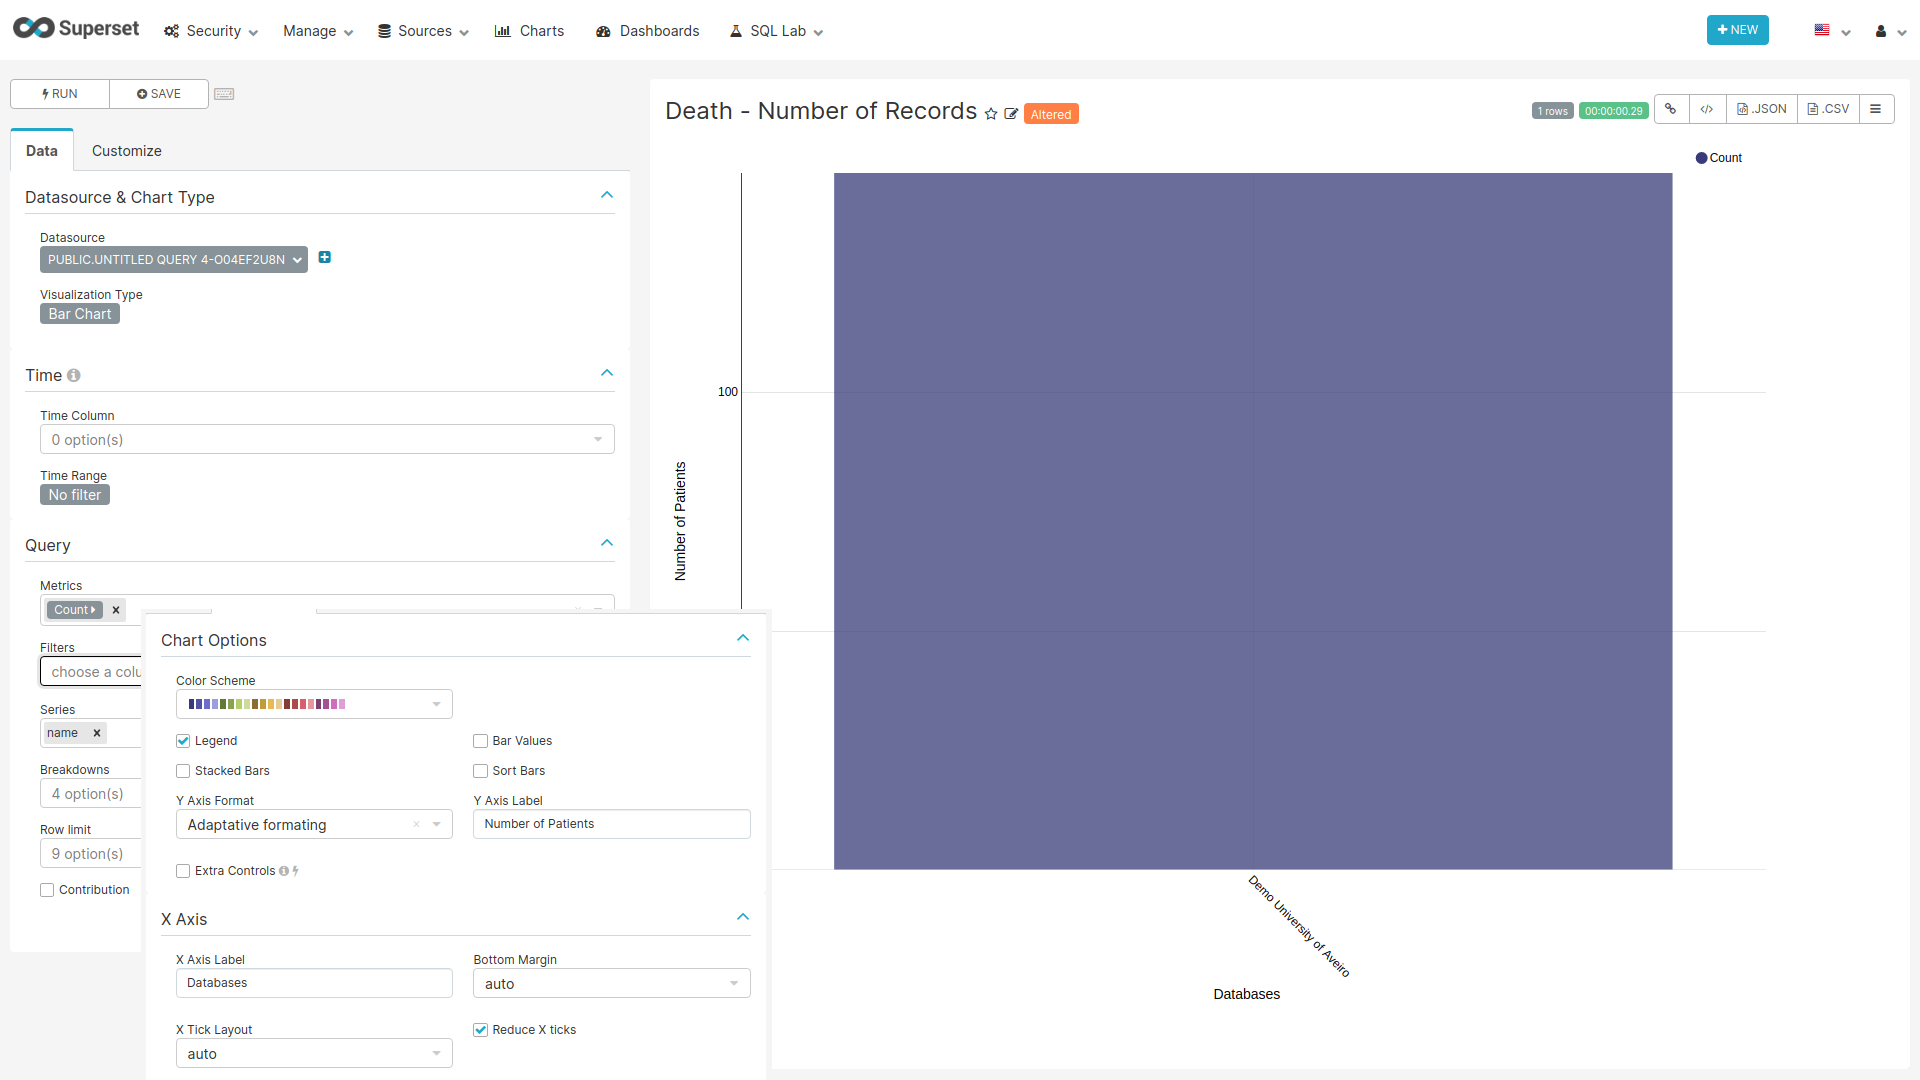
\includegraphics[width=1\linewidth]{images/07-death/02-number_of_records} \caption{Settings for creating the Number of Records chart}\label{fig:numberOfRecords}
\end{figure}

\hypertarget{sql-query-27}{%
\subsubsection*{SQL query}\label{sql-query-27}}
\addcontentsline{toc}{subsubsection}{SQL query}

\begin{Shaded}
\begin{Highlighting}[]
\KeywordTok{SELECT} \KeywordTok{source}\NormalTok{.name,}
\NormalTok{    count\_value,}
    \KeywordTok{source}\NormalTok{.acronym}
\KeywordTok{FROM} \KeywordTok{public}\NormalTok{.achilles\_results }\KeywordTok{AS}\NormalTok{ achilles}
\KeywordTok{INNER} \KeywordTok{JOIN} \KeywordTok{public}\NormalTok{.data\_source }\KeywordTok{AS} \KeywordTok{source} \KeywordTok{ON}\NormalTok{ achilles.data\_source\_id}\OperatorTok{=}\KeywordTok{source}\NormalTok{.}\KeywordTok{id}
\KeywordTok{WHERE}\NormalTok{ analysis\_id }\OperatorTok{=} \DecValTok{501}
\end{Highlighting}
\end{Shaded}

\hypertarget{chart-settings-29}{%
\subsubsection*{Chart settings}\label{chart-settings-29}}
\addcontentsline{toc}{subsubsection}{Chart settings}

\begin{itemize}
\tightlist
\item
  Data Tab

  \begin{itemize}
  \tightlist
  \item
    Datasource \& Chart Type

    \begin{itemize}
    \tightlist
    \item
      Visualization Type: Bar Chart
    \end{itemize}
  \item
    Time

    \begin{itemize}
    \tightlist
    \item
      Time range: No filter
    \end{itemize}
  \item
    Query

    \begin{itemize}
    \tightlist
    \item
      Metrics: MAX(count\_value) with label Count
    \item
      Series: name
    \end{itemize}
  \end{itemize}
\item
  Customize Tab

  \begin{itemize}
  \tightlist
  \item
    Chart Options

    \begin{itemize}
    \tightlist
    \item
      Y Axis Label: Number of Patients
    \end{itemize}
  \item
    X Axis

    \begin{itemize}
    \tightlist
    \item
      X Axis Label: Databases
    \item
      Reduce X ticks: on
    \end{itemize}
  \end{itemize}
\end{itemize}

\hypertarget{death-by-year-per-thousand-people}{%
\subsection*{Death By Year per Thousand People}\label{death-by-year-per-thousand-people}}
\addcontentsline{toc}{subsection}{Death By Year per Thousand People}

\begin{figure}
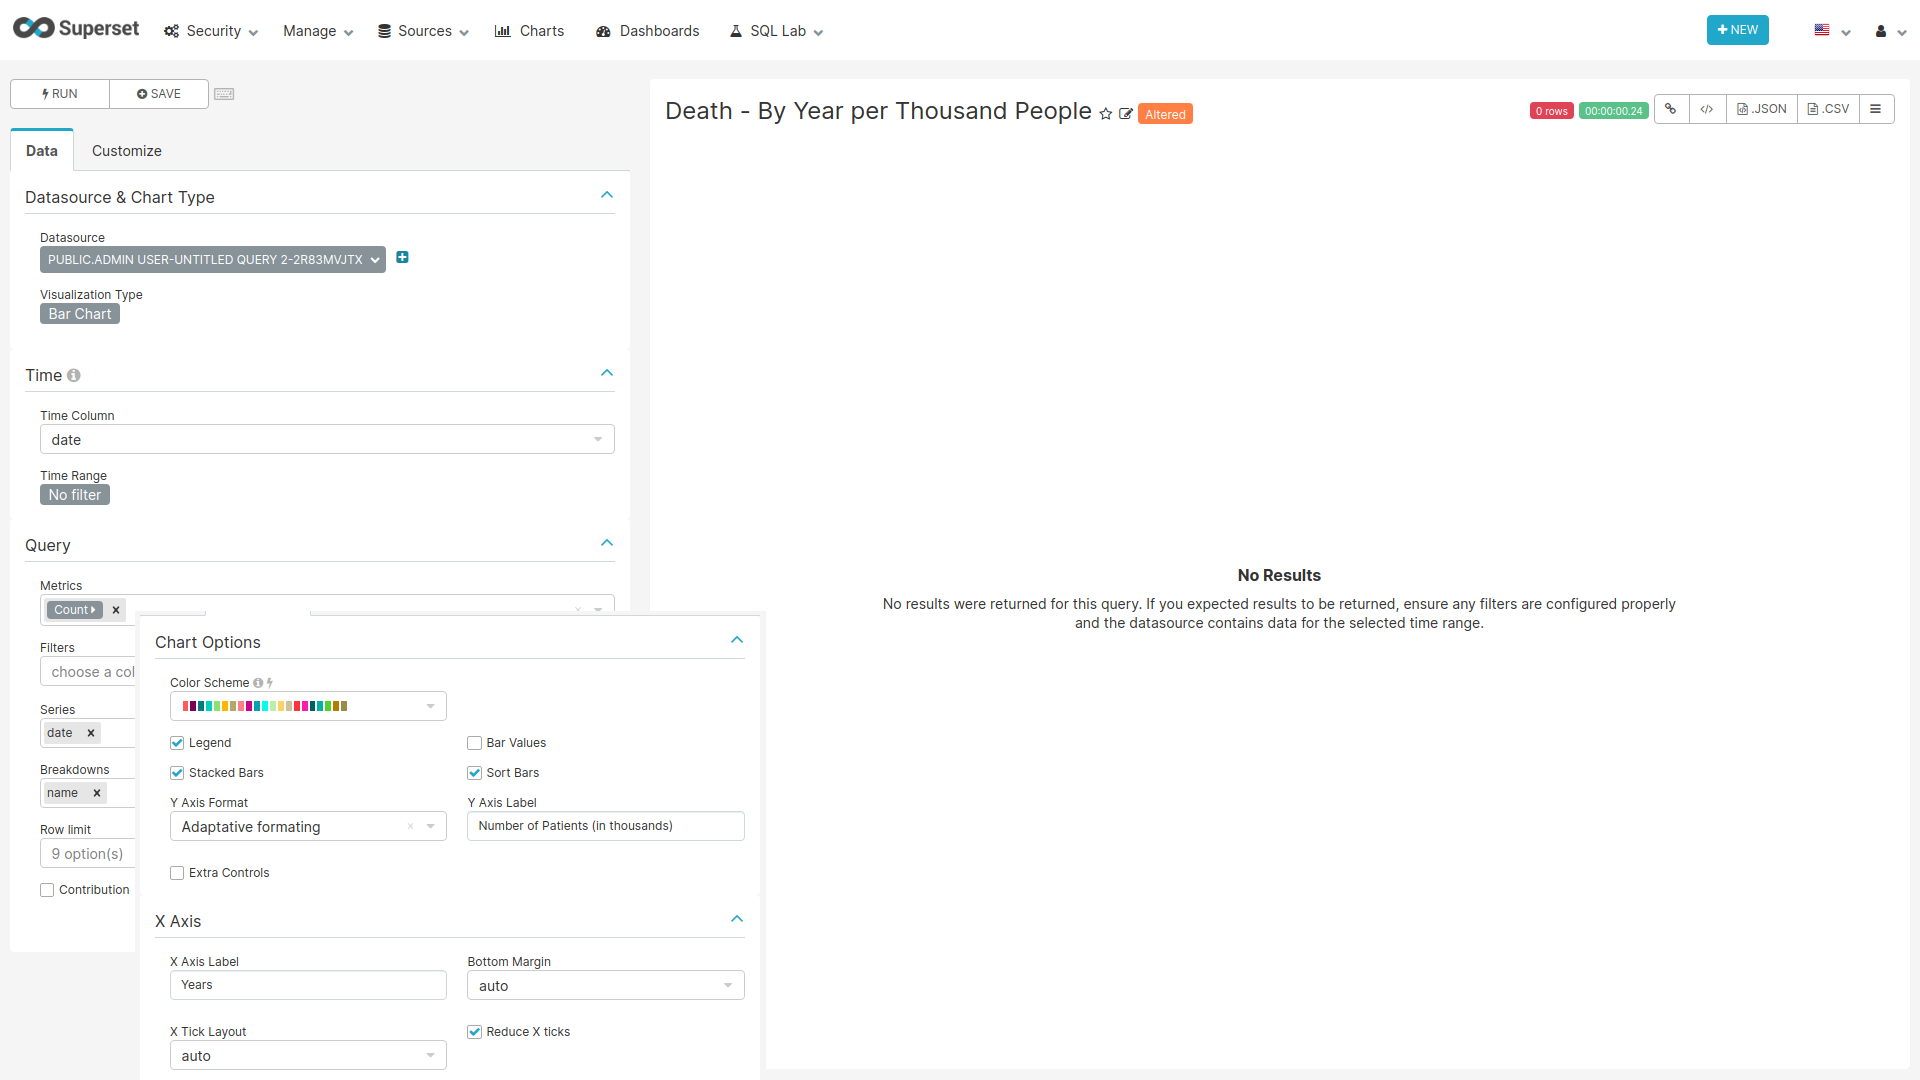
\includegraphics[width=1\linewidth]{images/07-death/03-deaths_by_year_per_thousand_people} \caption{Settings for creating the Death by Year per Thousand People chart}\label{fig:deathByYearPerThousandPeople}
\end{figure}

\hypertarget{sql-query-28}{%
\subsubsection*{SQL query}\label{sql-query-28}}
\addcontentsline{toc}{subsubsection}{SQL query}

\begin{Shaded}
\begin{Highlighting}[]
\KeywordTok{SELECT} \KeywordTok{source}\NormalTok{.name,}
    \KeywordTok{source}\NormalTok{.acronym,}
    \FunctionTok{EXTRACT}\NormalTok{(}\DataTypeTok{year} \KeywordTok{FROM} \FunctionTok{TO\_DATE}\NormalTok{(stratum\_1, }\StringTok{\textquotesingle{}YYYYMM\textquotesingle{}}\NormalTok{)) }\KeywordTok{AS} \DataTypeTok{Date}\NormalTok{,}
\NormalTok{    count\_value}
\KeywordTok{FROM} \KeywordTok{public}\NormalTok{.achilles\_results }\KeywordTok{as}\NormalTok{ achilles}
\KeywordTok{INNER} \KeywordTok{JOIN} \KeywordTok{public}\NormalTok{.data\_source }\KeywordTok{as} \KeywordTok{source} \KeywordTok{ON}\NormalTok{ achilles.data\_source\_id}\OperatorTok{=}\KeywordTok{source}\NormalTok{.}\KeywordTok{id}
\KeywordTok{WHERE}\NormalTok{ analysis\_id }\OperatorTok{=} \DecValTok{502}
\end{Highlighting}
\end{Shaded}

\hypertarget{chart-settings-30}{%
\subsubsection*{Chart settings}\label{chart-settings-30}}
\addcontentsline{toc}{subsubsection}{Chart settings}

\begin{itemize}
\tightlist
\item
  Data Tab

  \begin{itemize}
  \tightlist
  \item
    Datasource \& Chart Type

    \begin{itemize}
    \tightlist
    \item
      Visualization Type: Bar Chart
    \end{itemize}
  \item
    Time

    \begin{itemize}
    \tightlist
    \item
      Time range: No filter
    \end{itemize}
  \item
    Query

    \begin{itemize}
    \tightlist
    \item
      Metrics: MAX(count\_value) with label Count
    \item
      Series: date
    \item
      Breakdowns: name
    \end{itemize}
  \end{itemize}
\item
  Customize Tab

  \begin{itemize}
  \tightlist
  \item
    Chart Options

    \begin{itemize}
    \tightlist
    \item
      Stacked Bars: on
    \item
      Sort Bars: on
    \item
      Y Axis Label:Number of Patients (in thousands)
    \end{itemize}
  \item
    X Axis

    \begin{itemize}
    \tightlist
    \item
      X Axis Label: Years
    \item
      Reduce X ticks: on
    \end{itemize}
  \end{itemize}
\end{itemize}

\hypertarget{concepts-browser-deprecated}{%
\section{Concepts Browser {[}Deprecated{]}}\label{concepts-browser-deprecated}}

The concepts browser allows you to search for concepts by name or concept\_id in all the data sources you select. No exact number of patients or occurrences are provided but the magnitude of both.

\hypertarget{css-7}{%
\subsection*{CSS}\label{css-7}}
\addcontentsline{toc}{subsection}{CSS}

To hide the dashboard header insert the following css code to the \texttt{CSS} field on the edit page:

\begin{Shaded}
\begin{Highlighting}[]
\FunctionTok{.dashboard} \OperatorTok{\textgreater{}}\NormalTok{ div}\InformationTok{:not(}\FunctionTok{.dashboard{-}content}\InformationTok{)}\NormalTok{ \{  }\CommentTok{/* dashboard header */}
  \KeywordTok{display}\NormalTok{: }\DecValTok{none}\OperatorTok{;}
\NormalTok{\}}
\end{Highlighting}
\end{Shaded}

With this every time you want to edit the dashboard layout you have to either comment the CSS inserted
or remove it so the ``Edit Dashboard'' button can show again.

\hypertarget{data-source-and-domain-filters}{%
\subsection*{Data Source and Domain Filters}\label{data-source-and-domain-filters}}
\addcontentsline{toc}{subsection}{Data Source and Domain Filters}

\begin{figure}
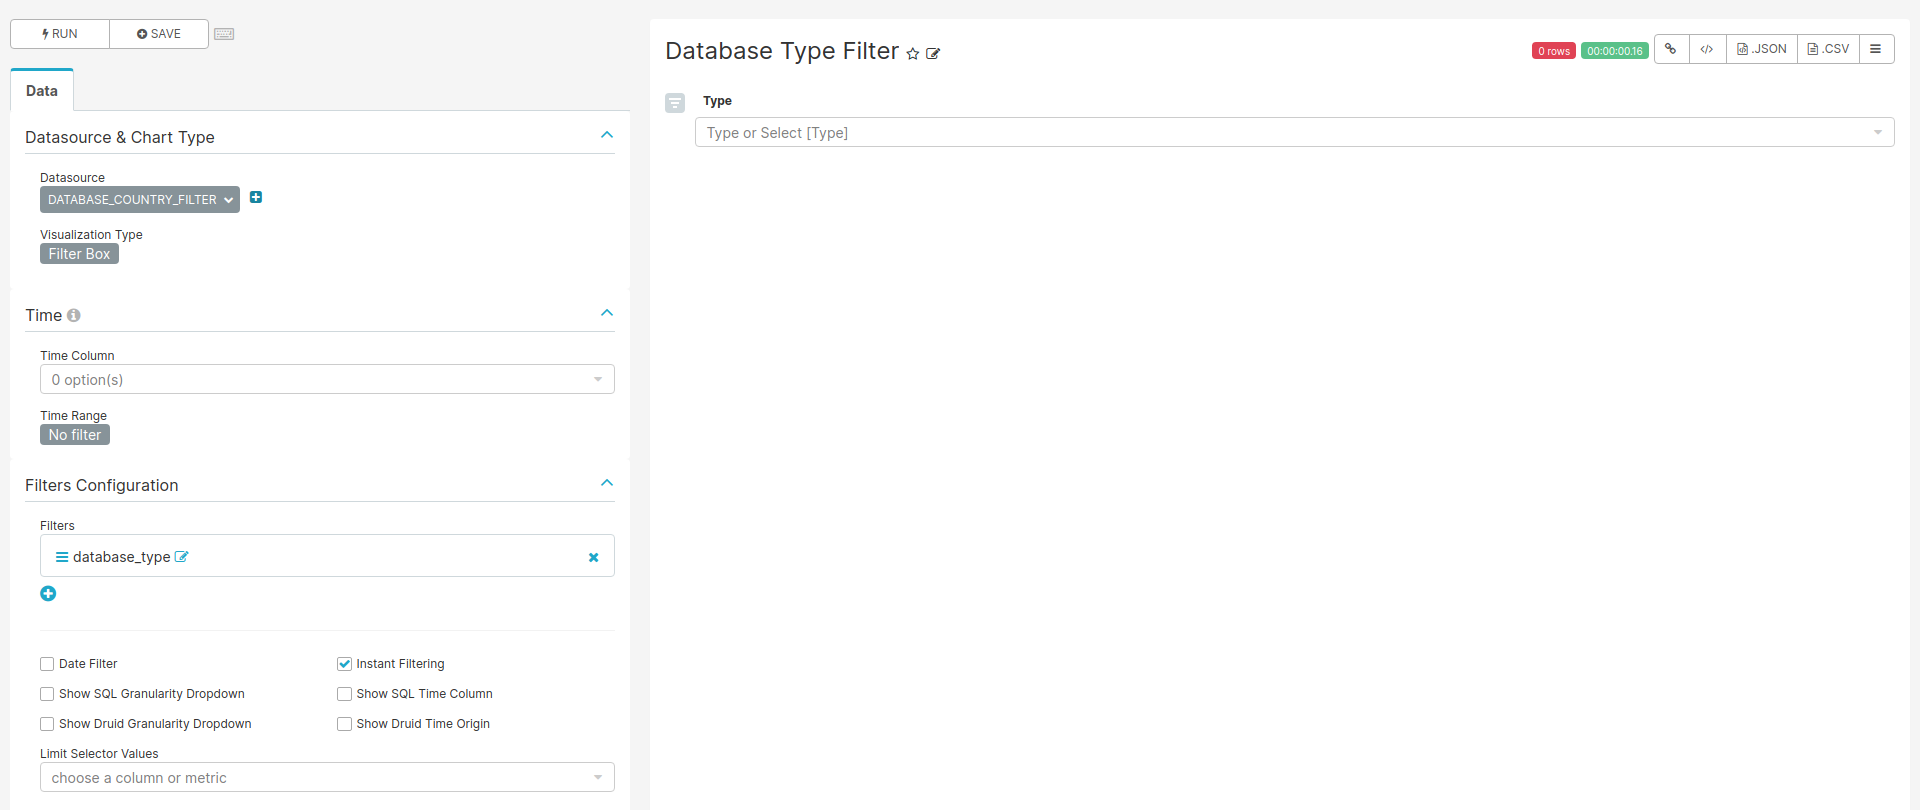
\includegraphics[width=1\linewidth]{images/08-concepts_browser/01-filters} \caption{Settings for creating the Data Source and Domain filter charts}\label{fig:filters}
\end{figure}

\textbf{For the filters to work the name of the fields to filter should match in all tables used on the charts of this dashboard.}

\hypertarget{sql-query-29}{%
\subsubsection*{SQL query}\label{sql-query-29}}
\addcontentsline{toc}{subsubsection}{SQL query}

\begin{Shaded}
\begin{Highlighting}[]
\KeywordTok{SELECT}\NormalTok{ concept\_name,}
\NormalTok{     domain\_id,}
     \KeywordTok{source}\NormalTok{.name }\KeywordTok{AS}\NormalTok{ source\_name,}
     \KeywordTok{source}\NormalTok{.acronym}
\KeywordTok{FROM}\NormalTok{ achilles\_results}
\KeywordTok{JOIN}\NormalTok{ concept }\KeywordTok{ON} \FunctionTok{cast}\NormalTok{(stratum\_1 }\KeywordTok{AS}\NormalTok{ BIGINT) }\OperatorTok{=}\NormalTok{ concept\_id}
\KeywordTok{INNER} \KeywordTok{JOIN} \KeywordTok{public}\NormalTok{.data\_source }\KeywordTok{AS} \KeywordTok{source} \KeywordTok{ON}\NormalTok{ data\_source\_id}\OperatorTok{=}\KeywordTok{source}\NormalTok{.}\KeywordTok{id}
\KeywordTok{WHERE}\NormalTok{ analysis\_id }\KeywordTok{in}\NormalTok{ (}\DecValTok{201}\NormalTok{, }\DecValTok{401}\NormalTok{, }\DecValTok{601}\NormalTok{, }\DecValTok{701}\NormalTok{, }\DecValTok{801}\NormalTok{, }\DecValTok{901}\NormalTok{, }\DecValTok{1001}\NormalTok{, }\DecValTok{1801}\NormalTok{, }\DecValTok{200}\NormalTok{, }\DecValTok{400}\NormalTok{, }\DecValTok{600}\NormalTok{, }\DecValTok{700}\NormalTok{, }\DecValTok{800}\NormalTok{, }\DecValTok{1800}\NormalTok{)}
\end{Highlighting}
\end{Shaded}

\hypertarget{chart-settings-31}{%
\subsubsection*{Chart settings}\label{chart-settings-31}}
\addcontentsline{toc}{subsubsection}{Chart settings}

\begin{itemize}
\tightlist
\item
  Data Tab

  \begin{itemize}
  \tightlist
  \item
    Datasource \& Chart Type

    \begin{itemize}
    \tightlist
    \item
      Visualization Type: Filter Box
    \end{itemize}
  \item
    Time

    \begin{itemize}
    \tightlist
    \item
      Time range: No filter
    \end{itemize}
  \item
    Filters Configuration

    \begin{itemize}
    \tightlist
    \item
      Filters:

      \begin{itemize}
      \tightlist
      \item
        source\_name or domain\_id
      \end{itemize}
    \item
      Date Filter: off
    \item
      Instant Filtering: on
    \end{itemize}
  \end{itemize}
\end{itemize}

\hypertarget{number-of-concepts}{%
\subsection*{Number of Concepts}\label{number-of-concepts}}
\addcontentsline{toc}{subsection}{Number of Concepts}

\begin{figure}
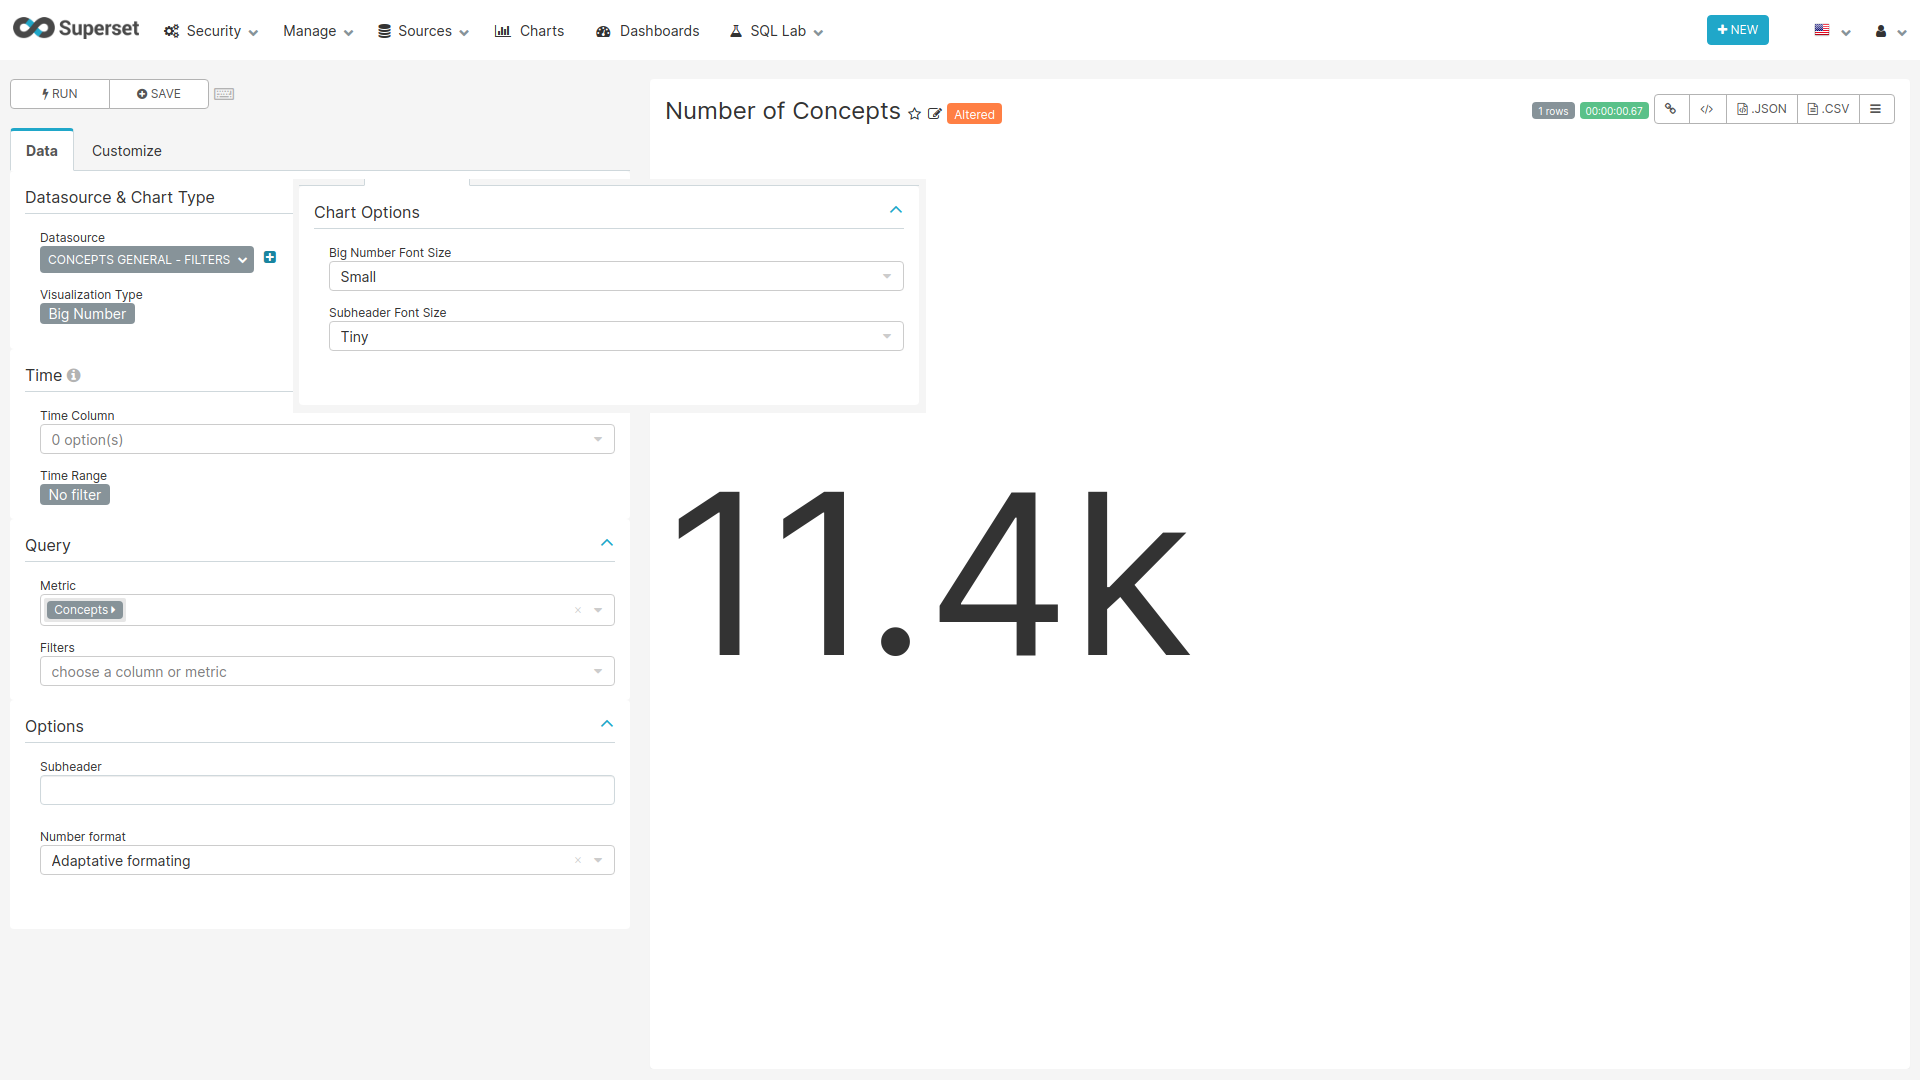
\includegraphics[width=1\linewidth]{images/08-concepts_browser/02-number_of_concepts} \caption{Settings for creating the Number of Concepts chart}\label{fig:numOfConcepts}
\end{figure}

\hypertarget{sql-query-30}{%
\subsubsection*{SQL Query}\label{sql-query-30}}
\addcontentsline{toc}{subsubsection}{SQL Query}

Same as \protect\hyperlink{Dataux5cux2520Sourceux5cux2520andux5cux2520Domainux5cux2520Filters}{Data Source and Domain filters} query

\hypertarget{chart-settings-32}{%
\subsubsection*{Chart settings}\label{chart-settings-32}}
\addcontentsline{toc}{subsubsection}{Chart settings}

\begin{itemize}
\tightlist
\item
  Data Tab

  \begin{itemize}
  \tightlist
  \item
    Datasource \& Chart Type

    \begin{itemize}
    \tightlist
    \item
      Visualization Type: Big Number
    \end{itemize}
  \item
    Time
    Time range: No filter
  \item
    Query

    \begin{itemize}
    \tightlist
    \item
      Metric: COUNT\_DISTINCT(concept\_name) with label Concepts
    \end{itemize}
  \end{itemize}
\item
  Customize Tab

  \begin{itemize}
  \tightlist
  \item
    Big Number Font Size: Small
  \item
    Subheader Font Size: Tiny
  \end{itemize}
\end{itemize}

\hypertarget{concept-browser-table-conceptbrowsertable}{%
\subsection*{Concept Browser Table \{\#conceptBrowserTable\}}\label{concept-browser-table-conceptbrowsertable}}
\addcontentsline{toc}{subsection}{Concept Browser Table \{\#conceptBrowserTable\}}

\begin{figure}
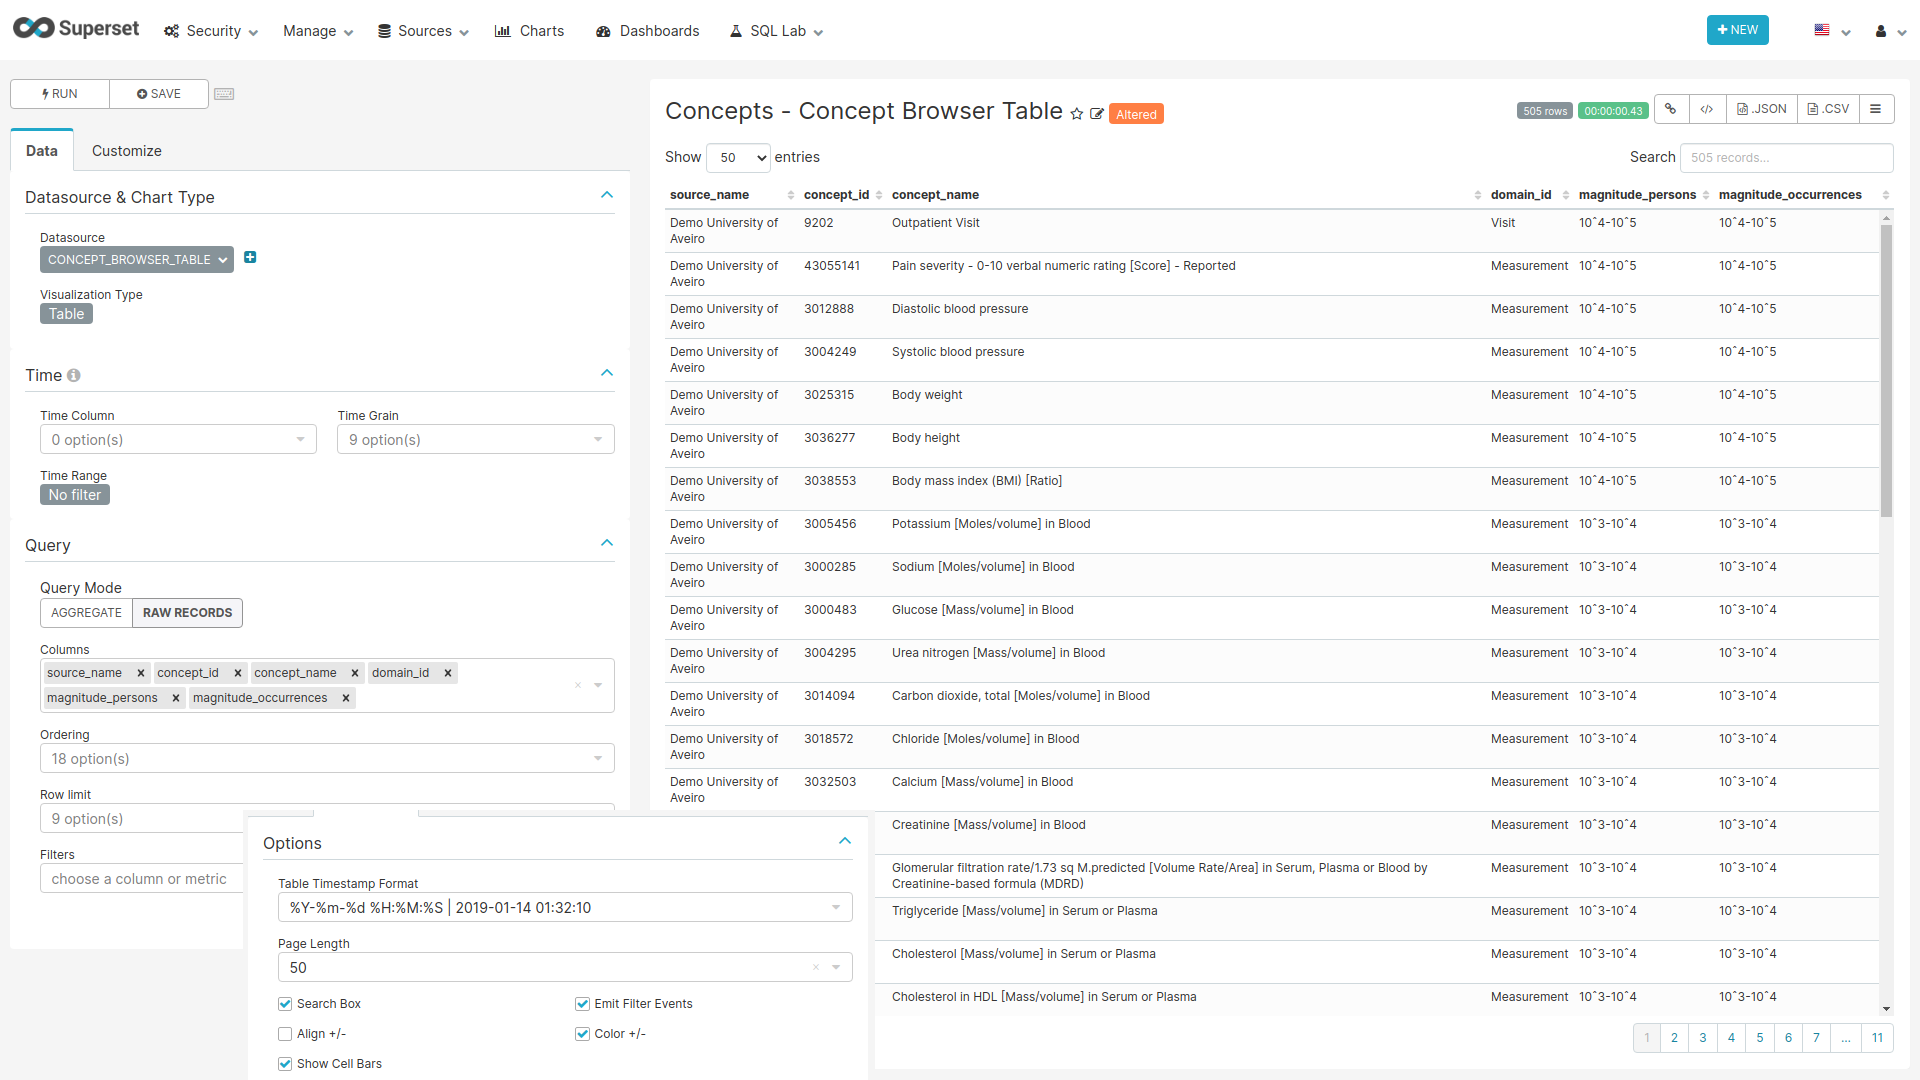
\includegraphics[width=1\linewidth]{images/08-concepts_browser/03-concepts_table} \caption{Settings for creating the Concepts Table chart}\label{fig:conceptsTable}
\end{figure}

\begin{Shaded}
\begin{Highlighting}[]
\KeywordTok{SELECT}
\NormalTok{    q1.concept\_id }\KeywordTok{AS}\NormalTok{ concept\_id,}
\NormalTok{    q1.concept\_name }\KeywordTok{AS}\NormalTok{ concept\_name,}
\NormalTok{    q1.domain\_id,}
    \KeywordTok{source}\NormalTok{.name }\KeywordTok{AS}\NormalTok{ source\_name,}
    \KeywordTok{source}\NormalTok{.acronym,}
    \FunctionTok{sum}\NormalTok{(q1.count\_value) }\KeywordTok{as} \OtherTok{"Occurrence\_count"}\NormalTok{,}
    \FunctionTok{sum}\NormalTok{(q1.count\_person) }\KeywordTok{as} \OtherTok{"Person\_count"}\NormalTok{,}
    \ControlFlowTok{CASE} 
        \ControlFlowTok{WHEN} \FunctionTok{sum}\NormalTok{(q1.count\_value)}\OperatorTok{\textless{}=}\DecValTok{10} \ControlFlowTok{THEN} \StringTok{\textquotesingle{}\textless{}=10\textquotesingle{}}
        \ControlFlowTok{WHEN} \FunctionTok{sum}\NormalTok{(q1.count\_value)}\OperatorTok{\textless{}=}\DecValTok{100} \ControlFlowTok{THEN} \StringTok{\textquotesingle{}11{-}10ˆ2\textquotesingle{}}
        \ControlFlowTok{WHEN} \FunctionTok{sum}\NormalTok{(q1.count\_value)}\OperatorTok{\textless{}=}\DecValTok{1000} \ControlFlowTok{THEN} \StringTok{\textquotesingle{}10ˆ2{-}10ˆ3\textquotesingle{}}
        \ControlFlowTok{WHEN} \FunctionTok{sum}\NormalTok{(q1.count\_value)}\OperatorTok{\textless{}=}\DecValTok{10000} \ControlFlowTok{THEN} \StringTok{\textquotesingle{}10ˆ3{-}10ˆ4\textquotesingle{}}
        \ControlFlowTok{WHEN} \FunctionTok{sum}\NormalTok{(q1.count\_value)}\OperatorTok{\textless{}=}\DecValTok{100000} \ControlFlowTok{THEN} \StringTok{\textquotesingle{}10ˆ4{-}10ˆ5\textquotesingle{}}
        \ControlFlowTok{WHEN} \FunctionTok{sum}\NormalTok{(q1.count\_value)}\OperatorTok{\textless{}=}\DecValTok{1000000} \ControlFlowTok{THEN} \StringTok{\textquotesingle{}10ˆ5{-}10ˆ6\textquotesingle{}}
        \ControlFlowTok{ELSE} \StringTok{\textquotesingle{}\textgreater{}10ˆ6\textquotesingle{}}
    \ControlFlowTok{END} \KeywordTok{as} \OtherTok{"magnitude\_occurrences"}\NormalTok{,}
    \ControlFlowTok{CASE} 
        \ControlFlowTok{WHEN} \FunctionTok{sum}\NormalTok{(q1.count\_person)}\OperatorTok{\textless{}=}\DecValTok{10} \ControlFlowTok{THEN} \StringTok{\textquotesingle{}\textless{}=10\textquotesingle{}}
        \ControlFlowTok{WHEN} \FunctionTok{sum}\NormalTok{(q1.count\_person)}\OperatorTok{\textless{}=}\DecValTok{100} \ControlFlowTok{THEN} \StringTok{\textquotesingle{}11{-}10ˆ2\textquotesingle{}}
        \ControlFlowTok{WHEN} \FunctionTok{sum}\NormalTok{(q1.count\_person)}\OperatorTok{\textless{}=}\DecValTok{1000} \ControlFlowTok{THEN} \StringTok{\textquotesingle{}10ˆ2{-}10ˆ3\textquotesingle{}}
        \ControlFlowTok{WHEN} \FunctionTok{sum}\NormalTok{(q1.count\_person)}\OperatorTok{\textless{}=}\DecValTok{10000} \ControlFlowTok{THEN} \StringTok{\textquotesingle{}10ˆ3{-}10ˆ4\textquotesingle{}}
        \ControlFlowTok{WHEN} \FunctionTok{sum}\NormalTok{(q1.count\_person)}\OperatorTok{\textless{}=}\DecValTok{100000} \ControlFlowTok{THEN} \StringTok{\textquotesingle{}10ˆ4{-}10ˆ5\textquotesingle{}}
        \ControlFlowTok{WHEN} \FunctionTok{sum}\NormalTok{(q1.count\_person)}\OperatorTok{\textless{}=}\DecValTok{1000000} \ControlFlowTok{THEN} \StringTok{\textquotesingle{}10ˆ5{-}10ˆ6\textquotesingle{}}
        \ControlFlowTok{ELSE} \StringTok{\textquotesingle{}\textgreater{}10ˆ6\textquotesingle{}}
    \ControlFlowTok{END} \KeywordTok{AS} \OtherTok{"magnitude\_persons"}
\KeywordTok{FROM}\NormalTok{ (}\KeywordTok{SELECT}\NormalTok{ analysis\_id,}
\NormalTok{             stratum\_1 concept\_id,}
\NormalTok{             data\_source\_id,}
\NormalTok{             concept\_name,}
\NormalTok{             domain\_id,}
\NormalTok{             count\_value, }\DecValTok{0} \KeywordTok{as}\NormalTok{ count\_person}
    \KeywordTok{FROM}\NormalTok{ achilles\_results}
    \KeywordTok{JOIN}\NormalTok{ concept }\KeywordTok{ON} \FunctionTok{cast}\NormalTok{(stratum\_1 }\KeywordTok{AS}\NormalTok{ BIGINT)}\OperatorTok{=}\NormalTok{concept\_id}
    \KeywordTok{WHERE}\NormalTok{ analysis\_id }\KeywordTok{in}\NormalTok{ (}\DecValTok{201}\NormalTok{, }\DecValTok{301}\NormalTok{, }\DecValTok{401}\NormalTok{, }\DecValTok{601}\NormalTok{, }\DecValTok{701}\NormalTok{, }\DecValTok{801}\NormalTok{, }\DecValTok{901}\NormalTok{, }\DecValTok{1001}\NormalTok{, }\DecValTok{1801}\NormalTok{)}
    \KeywordTok{UNION}\NormalTok{ (}\KeywordTok{SELECT}\NormalTok{  analysis\_id,}
\NormalTok{                   stratum\_1 concept\_id,}
\NormalTok{                   data\_source\_id,}
\NormalTok{                   concept\_name,}
\NormalTok{                   domain\_id,}
                   \DecValTok{0} \KeywordTok{as}\NormalTok{ count\_value,}
                   \FunctionTok{sum}\NormalTok{(count\_value) }\KeywordTok{as}\NormalTok{ count\_person}
            \KeywordTok{FROM}\NormalTok{  achilles\_results}
            \KeywordTok{JOIN}\NormalTok{ concept }\KeywordTok{on} \FunctionTok{cast}\NormalTok{(stratum\_1 }\KeywordTok{as}\NormalTok{ BIGINT)}\OperatorTok{=}\NormalTok{concept\_id}
            \KeywordTok{WHERE}\NormalTok{ analysis\_id }\KeywordTok{in}\NormalTok{ (}\DecValTok{202}\NormalTok{, }\DecValTok{401}\NormalTok{, }\DecValTok{601}\NormalTok{, }\DecValTok{701}\NormalTok{, }\DecValTok{801}\NormalTok{, }\DecValTok{901}\NormalTok{, }\DecValTok{1001}\NormalTok{, }\DecValTok{1801}\NormalTok{)}
            \KeywordTok{GROUP} \KeywordTok{BY}\NormalTok{ analysis\_id,stratum\_1,data\_source\_id,concept\_name,domain\_id) ) }\KeywordTok{as}\NormalTok{ q1}
    \KeywordTok{INNER} \KeywordTok{JOIN} \KeywordTok{public}\NormalTok{.data\_source }\KeywordTok{AS} \KeywordTok{source} \KeywordTok{ON}\NormalTok{ q1.data\_source\_id}\OperatorTok{=}\KeywordTok{source}\NormalTok{.}\KeywordTok{id}
\KeywordTok{GROUP} \KeywordTok{BY}\NormalTok{ q1.concept\_id,q1.concept\_name,q1.domain\_id,}\KeywordTok{source}\NormalTok{.name, acronym}
\KeywordTok{ORDER} \KeywordTok{BY} \OtherTok{"Person\_count"} \KeywordTok{desc}
\end{Highlighting}
\end{Shaded}

\hypertarget{chart-settings-33}{%
\subsubsection*{Chart settings}\label{chart-settings-33}}
\addcontentsline{toc}{subsubsection}{Chart settings}

\begin{itemize}
\tightlist
\item
  Data Tab

  \begin{itemize}
  \tightlist
  \item
    Datasource \& Chart Type

    \begin{itemize}
    \tightlist
    \item
      Visualization Type: Table
    \end{itemize}
  \item
    Time

    \begin{itemize}
    \tightlist
    \item
      Time range: No filter
    \end{itemize}
  \item
    Query

    \begin{itemize}
    \tightlist
    \item
      Query Mode: Raw Records
    \item
      Columns: source\_name, concept\_id, concept\_name, domain\_id, magnitude\_persons, magnitude\_occurrences
    \end{itemize}
  \end{itemize}
\item
  Customize Tab

  \begin{itemize}
  \tightlist
  \item
    Options

    \begin{itemize}
    \tightlist
    \item
      Table Timestamps Format: \%Y-\%m-\%d \%H:\%M:\%S \textbar{} 2019-01-14 01:32:10
    \item
      Page Length: 50
    \item
      Search Box: on
    \item
      Emit Filter Events: on
    \end{itemize}
  \end{itemize}
\end{itemize}

\hypertarget{provenance-deprecated}{%
\section{Provenance {[}Deprecated{]}}\label{provenance-deprecated}}

This Dashboard shows the provenance of the data in the different data domains.

\hypertarget{css-8}{%
\subsection*{CSS}\label{css-8}}
\addcontentsline{toc}{subsection}{CSS}

To hide the dashboard header insert the following css code to the \texttt{CSS} field on the edit page:

\begin{Shaded}
\begin{Highlighting}[]
\FunctionTok{.dashboard} \OperatorTok{\textgreater{}}\NormalTok{ div}\InformationTok{:not(}\FunctionTok{.dashboard{-}content}\InformationTok{)}\NormalTok{ \{  }\CommentTok{/* dashboard header */}
  \KeywordTok{display}\NormalTok{: }\DecValTok{none}\OperatorTok{;}
\NormalTok{\}}
\end{Highlighting}
\end{Shaded}

With this every time you want to edit the dashboard layout you have to either comment the CSS inserted
or remove it so the ``Edit Dashboard'' button can show again.

\hypertarget{data-source-filter-5}{%
\subsection*{Data Source Filter}\label{data-source-filter-5}}
\addcontentsline{toc}{subsection}{Data Source Filter}

\begin{figure}
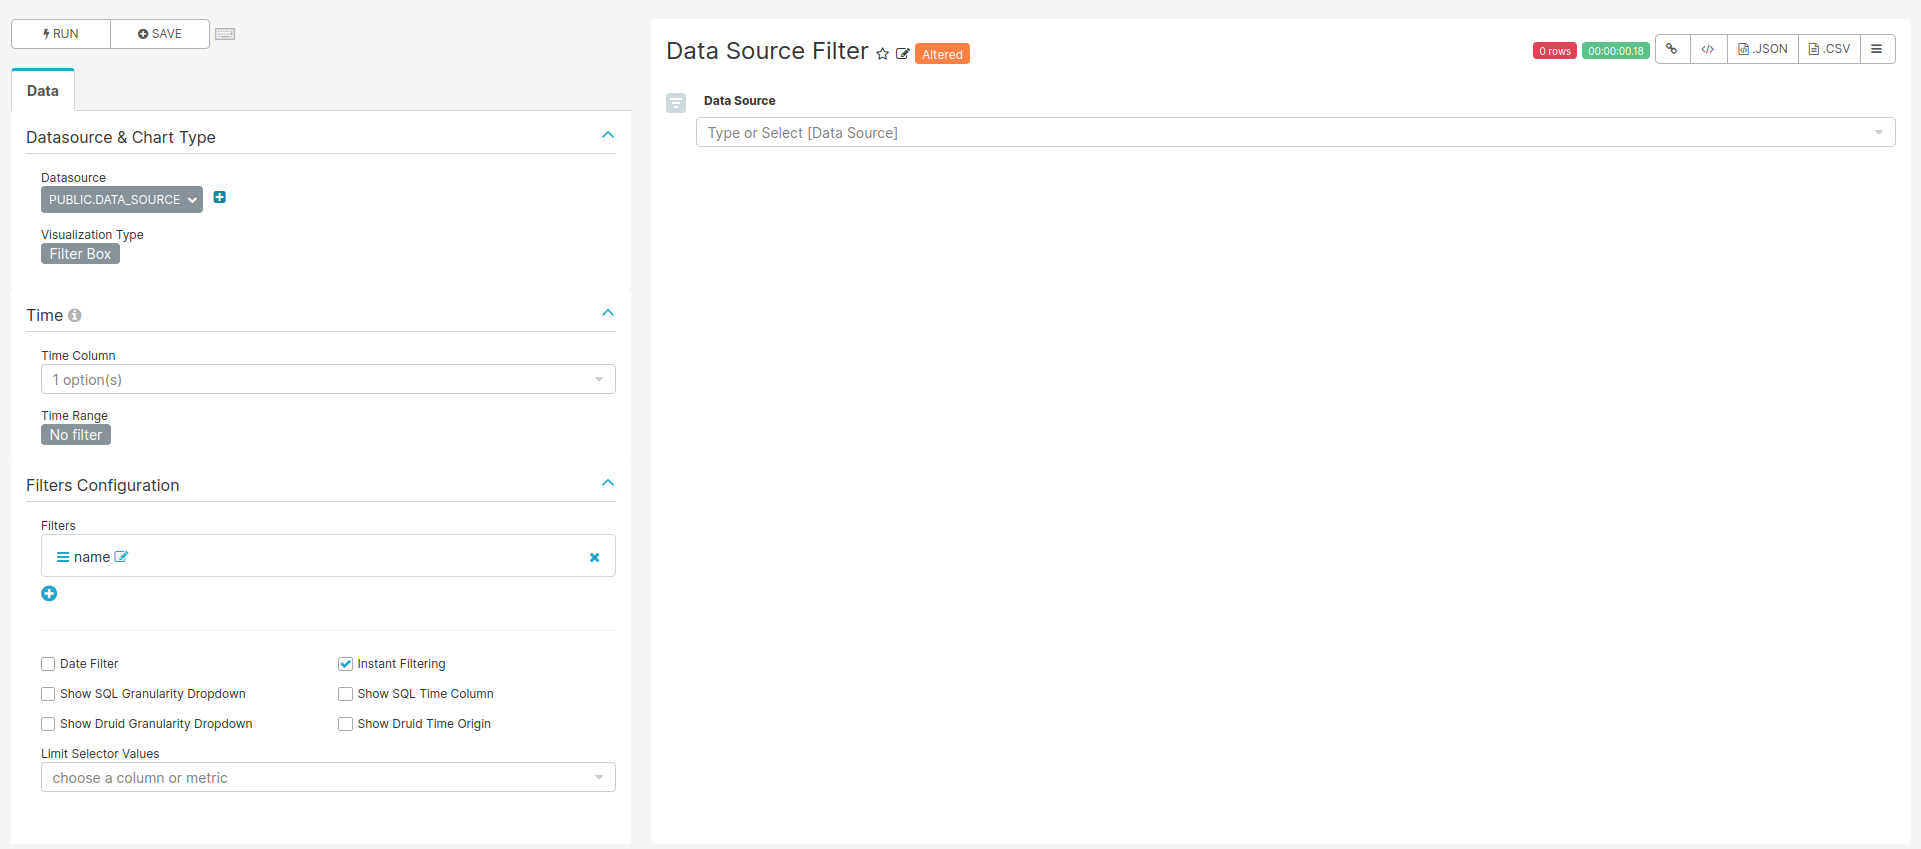
\includegraphics[width=1\linewidth]{images/shared/data_source_filter} \caption{Settings for creating the Data Source filter chart}\label{fig:dataSourceFilter}
\end{figure}

\textbf{For the filter to work the name of the fields to filter should match in all tables used on the charts of this dashboard.}

\hypertarget{sql-query-31}{%
\subsubsection*{SQL query}\label{sql-query-31}}
\addcontentsline{toc}{subsubsection}{SQL query}

No SQL query, use the sql table \texttt{data\_source} of the \texttt{achilles} database.

\hypertarget{chart-settings-34}{%
\subsubsection*{Chart settings}\label{chart-settings-34}}
\addcontentsline{toc}{subsubsection}{Chart settings}

\begin{itemize}
\tightlist
\item
  Data Tab

  \begin{itemize}
  \tightlist
  \item
    Datasource \& Chart Type

    \begin{itemize}
    \tightlist
    \item
      Visualization Type: Filter Box
    \end{itemize}
  \item
    Time

    \begin{itemize}
    \tightlist
    \item
      Time range: No filter
    \end{itemize}
  \item
    Filters Configuration

    \begin{itemize}
    \tightlist
    \item
      Filters:

      \begin{itemize}
      \tightlist
      \item
        name
      \end{itemize}
    \item
      Date Filter: off
    \item
      Instant Filtering: on
    \end{itemize}
  \end{itemize}
\end{itemize}

\hypertarget{condition-drug-procedure-device-measurement-observation-types-dataprovenancecharts}{%
\subsection*{Condition \& Drug \& Procedure \& Device \& Measurement \& Observation Types \{\#dataProvenanceCharts\}}\label{condition-drug-procedure-device-measurement-observation-types-dataprovenancecharts}}
\addcontentsline{toc}{subsection}{Condition \& Drug \& Procedure \& Device \& Measurement \& Observation Types \{\#dataProvenanceCharts\}}

\begin{figure}
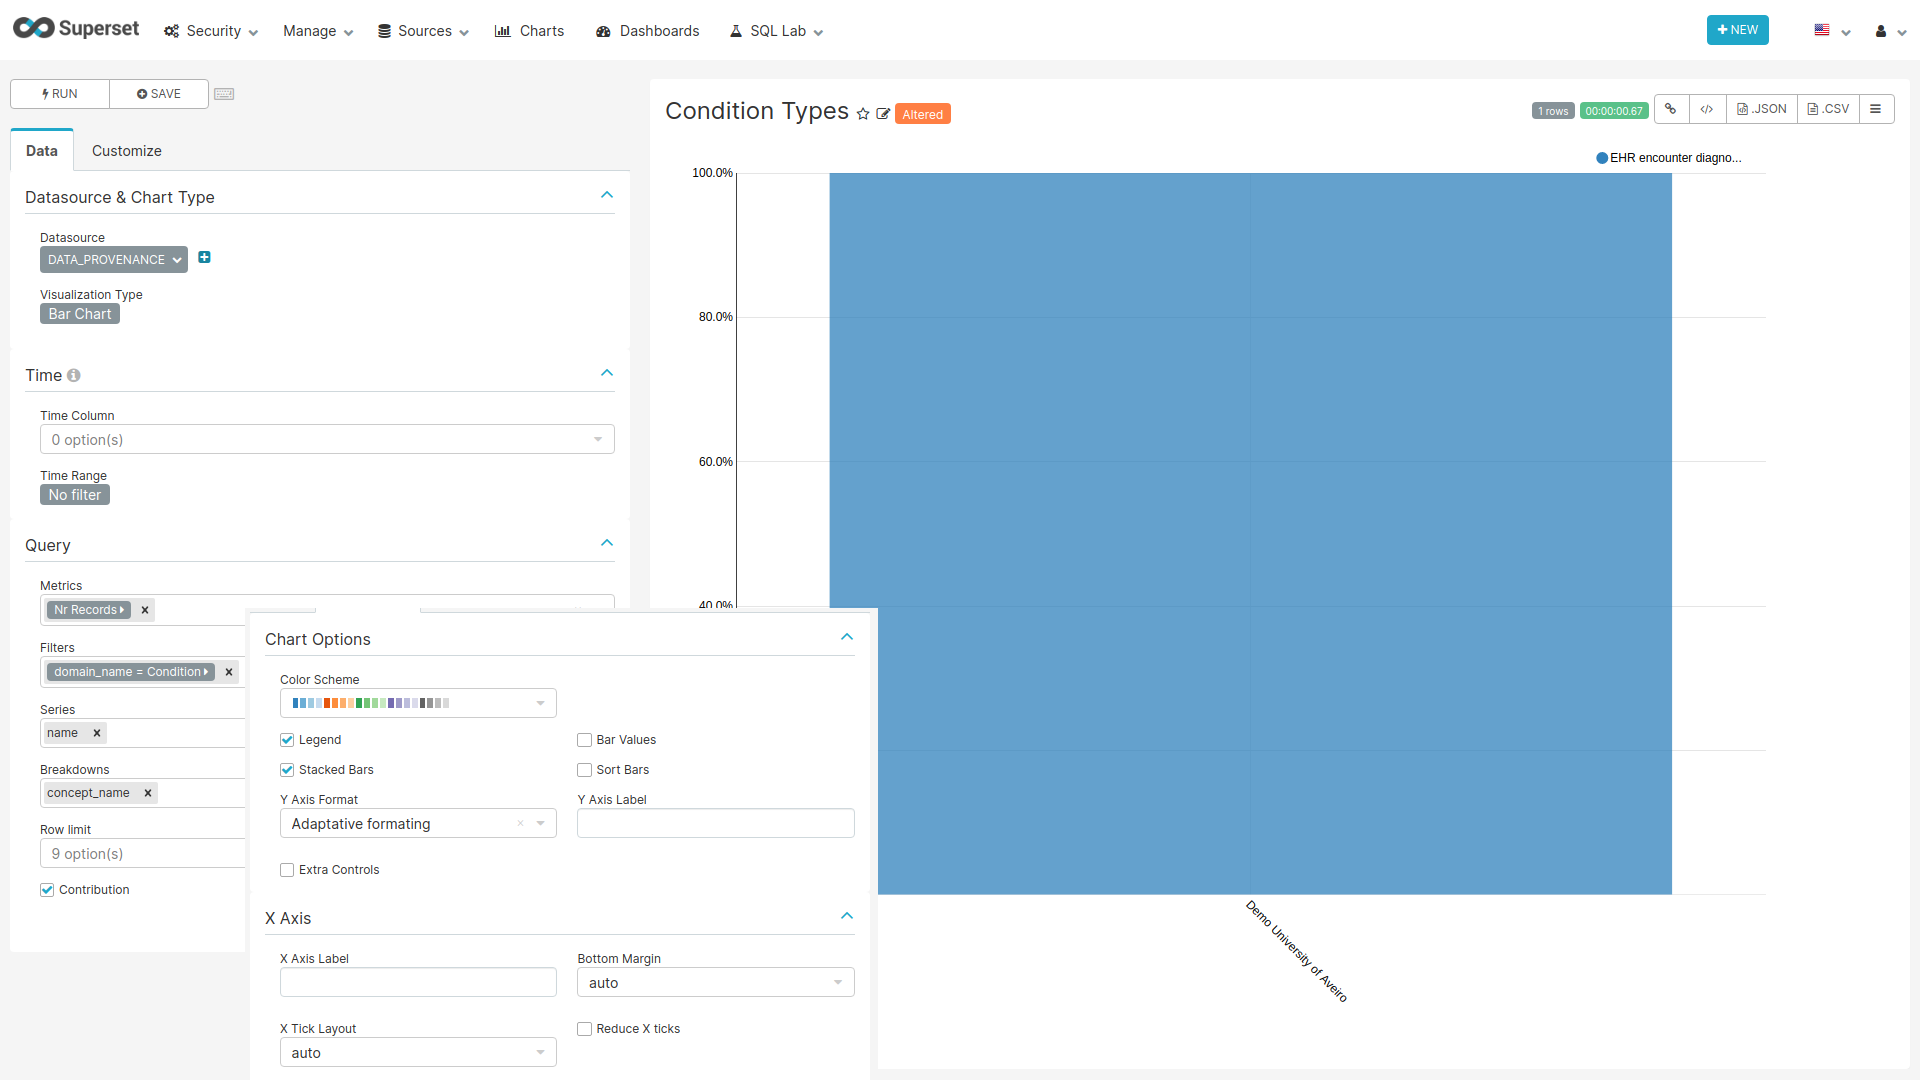
\includegraphics[width=1\linewidth]{images/09-provenance/02-condition_drug_procedure_device_measurement_observation_types} \caption{Settings for creating the Condition, Drug, Procedure, Device, Measurement and Observation charts}\label{fig:conditionDrugProcedureDeviceMeasurementObservationTypes}
\end{figure}

\hypertarget{sql-query-32}{%
\subsubsection*{SQL query}\label{sql-query-32}}
\addcontentsline{toc}{subsubsection}{SQL query}

All 6 charts use the same sql query.

\begin{Shaded}
\begin{Highlighting}[]
\KeywordTok{SELECT} \KeywordTok{source}\NormalTok{.name,}
    \KeywordTok{source}\NormalTok{.acronym,}
    \ControlFlowTok{CASE} \ControlFlowTok{WHEN}\NormalTok{ analysis\_id }\OperatorTok{=} \DecValTok{405} \ControlFlowTok{THEN} \StringTok{\textquotesingle{}Condition\textquotesingle{}}
    \ControlFlowTok{WHEN}\NormalTok{ analysis\_id }\OperatorTok{=} \DecValTok{605} \ControlFlowTok{THEN} \StringTok{\textquotesingle{}Procedure\textquotesingle{}}
    \ControlFlowTok{WHEN}\NormalTok{ analysis\_id }\OperatorTok{=} \DecValTok{705} \ControlFlowTok{THEN} \StringTok{\textquotesingle{}Drug\textquotesingle{}}
    \ControlFlowTok{WHEN}\NormalTok{ analysis\_id }\OperatorTok{=} \DecValTok{805} \ControlFlowTok{THEN} \StringTok{\textquotesingle{}Observation\textquotesingle{}}
    \ControlFlowTok{WHEN}\NormalTok{ analysis\_id }\OperatorTok{=} \DecValTok{1805} \ControlFlowTok{THEN} \StringTok{\textquotesingle{}Measurement\textquotesingle{}}
    \ControlFlowTok{WHEN}\NormalTok{ analysis\_id }\OperatorTok{=} \DecValTok{2105} \ControlFlowTok{THEN} \StringTok{\textquotesingle{}Device\textquotesingle{}}
    \ControlFlowTok{ELSE} \StringTok{\textquotesingle{}Other\textquotesingle{}} \ControlFlowTok{END} \KeywordTok{AS}\NormalTok{ domain\_name,}
\NormalTok{    concept\_name,}
    \FunctionTok{SUM}\NormalTok{(count\_value) }\KeywordTok{AS}\NormalTok{ num\_records}
\KeywordTok{FROM} \KeywordTok{public}\NormalTok{.achilles\_results }\KeywordTok{AS}\NormalTok{ achilles}
\KeywordTok{INNER} \KeywordTok{JOIN} \KeywordTok{public}\NormalTok{.data\_source }\KeywordTok{AS} \KeywordTok{source} \KeywordTok{ON}\NormalTok{ achilles.data\_source\_id}\OperatorTok{=}\KeywordTok{source}\NormalTok{.}\KeywordTok{id}
\KeywordTok{INNER} \KeywordTok{JOIN} \KeywordTok{public}\NormalTok{.concept }\KeywordTok{AS}\NormalTok{ c1 }\KeywordTok{ON} \FunctionTok{CAST}\NormalTok{(stratum\_2 }\KeywordTok{AS}\NormalTok{ BIGINT) }\OperatorTok{=}\NormalTok{ concept\_id}
\KeywordTok{WHERE}\NormalTok{ analysis\_id }\KeywordTok{IN}\NormalTok{ (}\DecValTok{405}\NormalTok{,}\DecValTok{605}\NormalTok{,}\DecValTok{705}\NormalTok{,}\DecValTok{805}\NormalTok{,}\DecValTok{1805}\NormalTok{,}\DecValTok{2105}\NormalTok{)}
\KeywordTok{GROUP} \KeywordTok{BY} \KeywordTok{source}\NormalTok{.name, }\KeywordTok{source}\NormalTok{.acronym, concept\_name, }
    \ControlFlowTok{CASE} \ControlFlowTok{WHEN}\NormalTok{ analysis\_id }\OperatorTok{=} \DecValTok{405} \ControlFlowTok{THEN} \StringTok{\textquotesingle{}Condition\textquotesingle{}}
    \ControlFlowTok{WHEN}\NormalTok{ analysis\_id }\OperatorTok{=} \DecValTok{605} \ControlFlowTok{THEN} \StringTok{\textquotesingle{}Procedure\textquotesingle{}}
    \ControlFlowTok{WHEN}\NormalTok{ analysis\_id }\OperatorTok{=} \DecValTok{705} \ControlFlowTok{THEN} \StringTok{\textquotesingle{}Drug\textquotesingle{}}
    \ControlFlowTok{WHEN}\NormalTok{ analysis\_id }\OperatorTok{=} \DecValTok{805} \ControlFlowTok{THEN} \StringTok{\textquotesingle{}Observation\textquotesingle{}}
    \ControlFlowTok{WHEN}\NormalTok{ analysis\_id }\OperatorTok{=} \DecValTok{1805} \ControlFlowTok{THEN} \StringTok{\textquotesingle{}Measurement\textquotesingle{}}
    \ControlFlowTok{WHEN}\NormalTok{ analysis\_id }\OperatorTok{=} \DecValTok{2105} \ControlFlowTok{THEN} \StringTok{\textquotesingle{}Device\textquotesingle{}}
    \ControlFlowTok{ELSE} \StringTok{\textquotesingle{}Other\textquotesingle{}} \ControlFlowTok{END}
\end{Highlighting}
\end{Shaded}

\hypertarget{chart-settings-35}{%
\subsubsection*{Chart settings}\label{chart-settings-35}}
\addcontentsline{toc}{subsubsection}{Chart settings}

\begin{itemize}
\tightlist
\item
  Data Tab

  \begin{itemize}
  \tightlist
  \item
    Datasource \& Chart Type

    \begin{itemize}
    \tightlist
    \item
      Visualization Type: Bar Chart
    \end{itemize}
  \item
    Time

    \begin{itemize}
    \tightlist
    \item
      Time range: No filter
    \end{itemize}
  \item
    Query

    \begin{itemize}
    \tightlist
    \item
      Metrics: SUM(num\_records) with label Nr Records
    \item
      Filters: domain\_name=Condition or domain\_name=Drug or domain\_name=Procedure or domain\_name=Device or domain\_name=Measurement or domain\_name=Observation
    \item
      Series: name
    \item
      Breakdowns: concept\_name
    \item
      Contribution: on
    \end{itemize}
  \end{itemize}
\item
  Customize Tab

  \begin{itemize}
  \tightlist
  \item
    Chart Options

    \begin{itemize}
    \tightlist
    \item
      Stacked Bars: on
    \end{itemize}
  \end{itemize}
\end{itemize}

\hypertarget{data-domains-deprecated}{%
\section{Data Domains {[}Deprecated{]}}\label{data-domains-deprecated}}

\hypertarget{css-9}{%
\subsection*{CSS}\label{css-9}}
\addcontentsline{toc}{subsection}{CSS}

To hide the dashboard header insert the following css code to the \texttt{CSS} field on the edit page:

\begin{Shaded}
\begin{Highlighting}[]
\FunctionTok{.dashboard} \OperatorTok{\textgreater{}}\NormalTok{ div}\InformationTok{:not(}\FunctionTok{.dashboard{-}content}\InformationTok{)}\NormalTok{ \{  }\CommentTok{/* dashboard header */}
  \KeywordTok{display}\NormalTok{: }\DecValTok{none}\OperatorTok{;}
\NormalTok{\}}
\end{Highlighting}
\end{Shaded}

With this every time you want to edit the dashboard layout you have to either comment the CSS inserted
or remove it so the ``Edit Dashboard'' button can show again.

\hypertarget{data-source-filter-6}{%
\subsection*{Data Source Filter}\label{data-source-filter-6}}
\addcontentsline{toc}{subsection}{Data Source Filter}

\begin{figure}
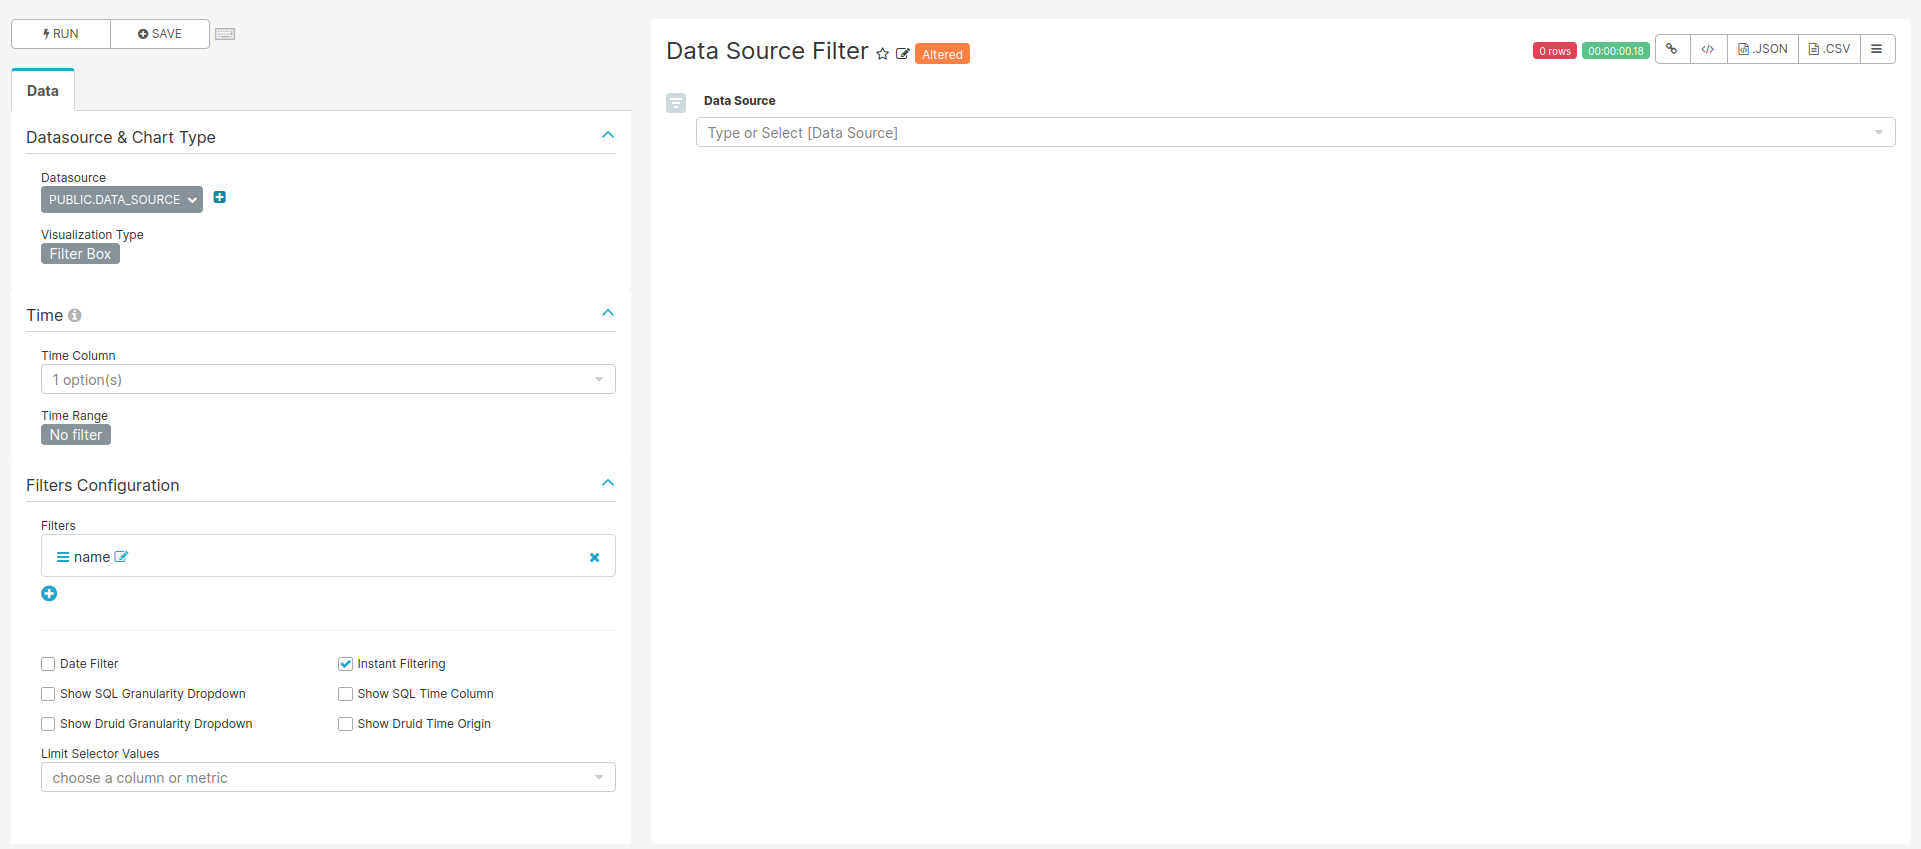
\includegraphics[width=1\linewidth]{images/shared/data_source_filter} \caption{Settings for creating the Data Source filter chart}\label{fig:dataSourceFilter}
\end{figure}

\textbf{For the filter to work the name of the fields to filter should match in all tables used on the charts of this dashboard.}

\hypertarget{sql-query-33}{%
\subsubsection*{SQL query}\label{sql-query-33}}
\addcontentsline{toc}{subsubsection}{SQL query}

No SQL query, use the sql table \texttt{data\_source} of the \texttt{achilles} database.

\hypertarget{chart-settings-36}{%
\subsubsection*{Chart settings}\label{chart-settings-36}}
\addcontentsline{toc}{subsubsection}{Chart settings}

\begin{itemize}
\tightlist
\item
  Data Tab

  \begin{itemize}
  \tightlist
  \item
    Datasource \& Chart Type

    \begin{itemize}
    \tightlist
    \item
      Visualization Type: Filter Box
    \end{itemize}
  \item
    Time

    \begin{itemize}
    \tightlist
    \item
      Time range: No filter
    \end{itemize}
  \item
    Filters Configuration

    \begin{itemize}
    \tightlist
    \item
      Filters:

      \begin{itemize}
      \tightlist
      \item
        name
      \end{itemize}
    \item
      Date Filter: off
    \item
      Instant Filtering: on
    \end{itemize}
  \end{itemize}
\end{itemize}

\hypertarget{average-number-of-records-per-person-avgrecordsperperson}{%
\subsection*{Average Number of Records per Person \{\#avgRecordsPerPerson\}}\label{average-number-of-records-per-person-avgrecordsperperson}}
\addcontentsline{toc}{subsection}{Average Number of Records per Person \{\#avgRecordsPerPerson\}}

\begin{figure}
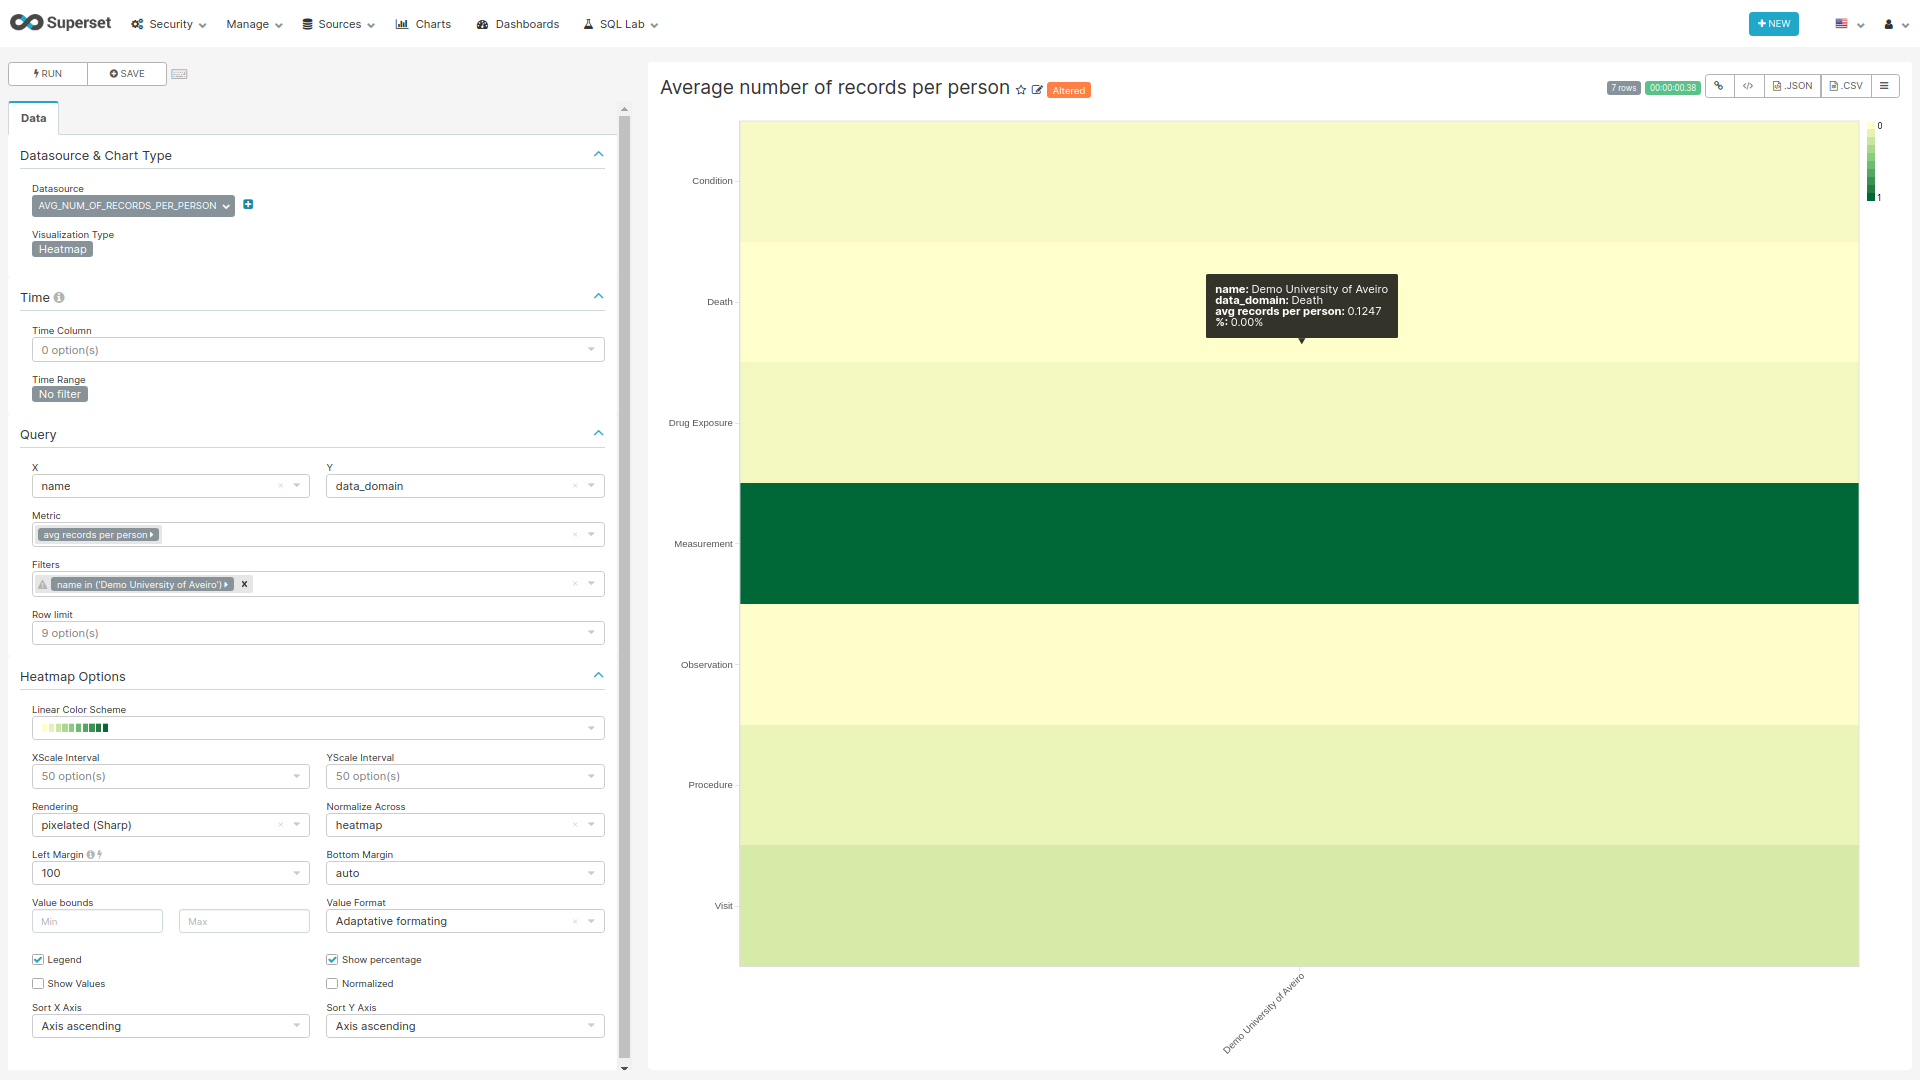
\includegraphics[width=1\linewidth]{images/10-data_domain/02-avg_records_per_person} \caption{Settings for creating the Data Source filter chart}\label{fig:unnamed-chunk-1}
\end{figure}

\hypertarget{sql-query-34}{%
\subsubsection*{SQL query}\label{sql-query-34}}
\addcontentsline{toc}{subsubsection}{SQL query}

\begin{Shaded}
\begin{Highlighting}[]
\KeywordTok{SELECT} 
    \KeywordTok{source}\NormalTok{.name,}
    \KeywordTok{source}\NormalTok{.acronym,}
    \ControlFlowTok{CASE} 
    \ControlFlowTok{WHEN}\NormalTok{ analysis\_id }\OperatorTok{=} \DecValTok{201} \ControlFlowTok{THEN} \StringTok{\textquotesingle{}Visit\textquotesingle{}}
    \ControlFlowTok{WHEN}\NormalTok{ analysis\_id }\OperatorTok{=} \DecValTok{401} \ControlFlowTok{THEN} \StringTok{\textquotesingle{}Condition\textquotesingle{}}
    \ControlFlowTok{WHEN}\NormalTok{ analysis\_id }\OperatorTok{=} \DecValTok{501} \ControlFlowTok{THEN} \StringTok{\textquotesingle{}Death\textquotesingle{}}
    \ControlFlowTok{WHEN}\NormalTok{ analysis\_id }\OperatorTok{=} \DecValTok{601} \ControlFlowTok{THEN} \StringTok{\textquotesingle{}Procedure\textquotesingle{}}
    \ControlFlowTok{WHEN}\NormalTok{ analysis\_id }\OperatorTok{=} \DecValTok{701} \ControlFlowTok{THEN} \StringTok{\textquotesingle{}Drug Exposure\textquotesingle{}}
    \ControlFlowTok{WHEN}\NormalTok{ analysis\_id }\OperatorTok{=} \DecValTok{801} \ControlFlowTok{THEN} \StringTok{\textquotesingle{}Observation\textquotesingle{}}
    \ControlFlowTok{WHEN}\NormalTok{ analysis\_id }\OperatorTok{=} \DecValTok{1801} \ControlFlowTok{THEN} \StringTok{\textquotesingle{}Measurement\textquotesingle{}}
    \ControlFlowTok{WHEN}\NormalTok{ analysis\_id }\OperatorTok{=} \DecValTok{2101} \ControlFlowTok{THEN} \StringTok{\textquotesingle{}Device\textquotesingle{}}
    \ControlFlowTok{WHEN}\NormalTok{ analysis\_id }\OperatorTok{=} \DecValTok{2201} \ControlFlowTok{THEN} \StringTok{\textquotesingle{}Note\textquotesingle{}}
    \ControlFlowTok{END} \KeywordTok{AS}\NormalTok{ Data\_Domain,}
    \FunctionTok{SUM}\NormalTok{(count\_value) }\OperatorTok{/}\FunctionTok{AVG}\NormalTok{(num\_persons) }\KeywordTok{AS} \OtherTok{"records\_per\_person"}
\KeywordTok{FROM} \KeywordTok{public}\NormalTok{.achilles\_results }\KeywordTok{AS}\NormalTok{ achilles}
\KeywordTok{INNER} \KeywordTok{JOIN} \KeywordTok{public}\NormalTok{.data\_source }\KeywordTok{AS} \KeywordTok{source} \KeywordTok{ON}\NormalTok{ achilles.data\_source\_id}\OperatorTok{=}\KeywordTok{source}\NormalTok{.}\KeywordTok{id}
\KeywordTok{INNER} \KeywordTok{JOIN}\NormalTok{ (}
  \KeywordTok{SELECT}\NormalTok{ data\_source\_id , count\_value }\KeywordTok{as}\NormalTok{ num\_persons}
  \KeywordTok{FROM}\NormalTok{ achilles\_results}
  \KeywordTok{WHERE}\NormalTok{ analysis\_id }\OperatorTok{=} \DecValTok{1}\NormalTok{) counts }\KeywordTok{ON}\NormalTok{ achilles.data\_source\_id }\OperatorTok{=}\NormalTok{ counts.data\_source\_id }
\KeywordTok{GROUP} \KeywordTok{BY}\NormalTok{ analysis\_id, }\KeywordTok{source}\NormalTok{.name, }\KeywordTok{source}\NormalTok{.acronym}
\KeywordTok{HAVING}\NormalTok{ analysis\_id }\KeywordTok{IN}\NormalTok{ (}\DecValTok{201}\NormalTok{, }\DecValTok{401}\NormalTok{, }\DecValTok{501}\NormalTok{, }\DecValTok{601}\NormalTok{, }\DecValTok{701}\NormalTok{, }\DecValTok{801}\NormalTok{, }\DecValTok{1801}\NormalTok{, }\DecValTok{2101}\NormalTok{, }\DecValTok{2201}\NormalTok{)}
\end{Highlighting}
\end{Shaded}

\hypertarget{chart-settings-37}{%
\subsubsection*{Chart settings}\label{chart-settings-37}}
\addcontentsline{toc}{subsubsection}{Chart settings}

\begin{itemize}
\tightlist
\item
  Data Tab

  \begin{itemize}
  \tightlist
  \item
    Datasource \& Chart Type

    \begin{itemize}
    \tightlist
    \item
      Visualization Type: Heatmap
    \end{itemize}
  \item
    Time

    \begin{itemize}
    \tightlist
    \item
      Time range: No filter
    \end{itemize}
  \item
    Query

    \begin{itemize}
    \tightlist
    \item
      X: name
    \item
      Y: data\_domain
    \item
      Metric: AVG(records\_per\_person) with a label avg records per person
    \item
      Row limit: None
    \end{itemize}
  \item
    Heatmap Options

    \begin{itemize}
    \tightlist
    \item
      Left Margin: 100
    \item
      Show Percentage: off
    \end{itemize}
  \end{itemize}
\end{itemize}

\hypertarget{development-instructions}{%
\chapter{Development Instructions}\label{development-instructions}}

\hypertarget{repository-description}{%
\subsection*{Repository Description}\label{repository-description}}
\addcontentsline{toc}{subsection}{Repository Description}

\hypertarget{code-documentation}{%
\chapter{Code Documentation}\label{code-documentation}}

  \bibliography{refs.bib}

\end{document}
